% Created 2021-10-11 Mon 13:18
% Intended LaTeX compiler: pdflatex
\documentclass[11pt]{article}
\usepackage[utf8]{inputenc}
\usepackage[T1]{fontenc}
\usepackage{graphicx}
\usepackage{grffile}
\usepackage{longtable}
\usepackage{wrapfig}
\usepackage{rotating}
\usepackage[normalem]{ulem}
\usepackage{amsmath}
\usepackage{textcomp}
\usepackage{amssymb}
\usepackage{capt-of}
\usepackage{hyperref}
% wrong resolution of image
% https://tex.stackexchange.com/questions/21627/image-from-includegraphics-showing-in-wrong-image-size?rq=1

%%%%%%%%%%%%%%%%%%%%%%%%%%%%%%%%%%%%%%
%% TIPS                                 %%
%%%%%%%%%%%%%%%%%%%%%%%%%%%%%%%%%%%%%%
% \substack{a\\b} for multiple lines text
% \usepackage{expl3}
% \expandafter\def\csname ver@l3regex.sty\endcsname{}
% \usepackage{pkgloader}
\usepackage[utf8]{inputenc}

% nfss error
% \usepackage[B1,T1]{fontenc}
\usepackage{fontspec}

% \usepackage[Emoticons]{ucharclasses}
\newfontfamily\DejaSans{DejaVu Sans}
% \setDefaultTransitions{\DejaSans}{}

% pdfplots will load xolor automatically without option
\usepackage[dvipsnames]{xcolor}

%                                                             ┳┳┓   ┓
%                                                             ┃┃┃┏┓╋┣┓
%                                                             ┛ ┗┗┻┗┛┗
% \usepackage{amsmath} mathtools loads the amsmath
\usepackage{amsmath}
\usepackage{mathtools}

\usepackage{amsthm}
\usepackage{amsbsy}

%\usepackage{commath}

\usepackage{amssymb}

\usepackage{mathrsfs}
%\usepackage{mathabx}
\usepackage{stmaryrd}
\usepackage{empheq}

\usepackage{scalerel}
\usepackage{stackengine}
\usepackage{stackrel}



\usepackage{nicematrix}
\usepackage{tensor}
\usepackage{blkarray}
\usepackage{siunitx}
\usepackage[f]{esvect}

% centering \not on a letter
\usepackage{slashed}
\usepackage[makeroom]{cancel}

%\usepackage{merriweather}
\usepackage{unicode-math}
\setmainfont{TeX Gyre Pagella}
% \setmathfont{STIX}
%\setmathfont{texgyrepagella-math.otf}
%\setmathfont{Libertinus Math}
\setmathfont{Latin Modern Math}

 % \setmathfont[range={\smwhtdiamond,\enclosediamond,\varlrtriangle}]{Latin Modern Math}
\setmathfont[range={\rightrightarrows,\twoheadrightarrow,\leftrightsquigarrow,\triangledown,\vartriangle,\precneq,\succneq,\prec,\succ,\preceq,\succeq,\tieconcat}]{XITS Math}
 \setmathfont[range={\int,\setminus}]{Libertinus Math}
 % \setmathfont[range={\mathalpha}]{TeX Gyre Pagella Math}
%\setmathfont[range={\mitA,\mitB,\mitC,\mitD,\mitE,\mitF,\mitG,\mitH,\mitI,\mitJ,\mitK,\mitL,\mitM,\mitN,\mitO,\mitP,\mitQ,\mitR,\mitS,\mitT,\mitU,\mitV,\mitW,\mitX,\mitY,\mitZ,\mita,\mitb,\mitc,\mitd,\mite,\mitf,\mitg,\miti,\mitj,\mitk,\mitl,\mitm,\mitn,\mito,\mitp,\mitq,\mitr,\mits,\mitt,\mitu,\mitv,\mitw,\mitx,\mity,\mitz}]{TeX Gyre Pagella Math}
% unicode is not good at this!
%\let\nmodels\nvDash

 \usepackage{wasysym}

 % for wide hat
 \DeclareSymbolFont{yhlargesymbols}{OMX}{yhex}{m}{n} \DeclareMathAccent{\what}{\mathord}{yhlargesymbols}{"62}

%                                                               ┏┳┓•┓
%                                                                ┃ ┓┃┏┓
%                                                                ┻ ┗┛┗┗

\usepackage{pgfplots}
\pgfplotsset{compat=1.18}
\usepackage{tikz}
\usepackage{tikz-cd}
\tikzcdset{scale cd/.style={every label/.append style={scale=#1},
    cells={nodes={scale=#1}}}}
% TODO: discard qtree and use forest
% \usepackage{tikz-qtree}
\usepackage{forest}

\usetikzlibrary{arrows,positioning,calc,fadings,decorations,matrix,decorations,shapes.misc}
%setting from geogebra
\definecolor{ccqqqq}{rgb}{0.8,0,0}

%                                                          ┳┳┓•    ┓┓
%                                                          ┃┃┃┓┏┏┏┓┃┃┏┓┏┓┏┓┏┓┓┏┏
%                                                          ┛ ┗┗┛┗┗ ┗┗┗┻┛┗┗ ┗┛┗┻┛
%\usepackage{twemojis}
\usepackage[most]{tcolorbox}
\usepackage{threeparttable}
\usepackage{tabularx}

\usepackage{enumitem}
\usepackage[indLines=false]{algpseudocodex}
\usepackage[]{algorithm2e}
% \SetKwComment{Comment}{/* }{ */}
% \algrenewcommand\algorithmicrequire{\textbf{Input:}}
% \algrenewcommand\algorithmicensure{\textbf{Output:}}
% wrong with preview
\usepackage{subcaption}
\usepackage{caption}
% {\aunclfamily\Huge}
\usepackage{auncial}

\usepackage{float}

\usepackage{fancyhdr}

\usepackage{ifthen}
\usepackage{xargs}

\definecolor{mintedbg}{rgb}{0.99,0.99,0.99}
\usepackage[cachedir=\detokenize{~/miscellaneous/trash}]{minted}
\setminted{breaklines,
  mathescape,
  bgcolor=mintedbg,
  fontsize=\footnotesize,
  frame=single,
  linenos}
\usemintedstyle{xcode}
\usepackage{tcolorbox}
\usepackage{etoolbox}



\usepackage{imakeidx}
\usepackage{hyperref}
\usepackage{soul}
\usepackage{framed}

% don't use this for preview
%\usepackage[margin=1.5in]{geometry}
% \usepackage{geometry}
% \geometry{legalpaper, landscape, margin=1in}
\usepackage[font=itshape]{quoting}

%\LoadPackagesNow
%\usepackage[xetex]{preview}
%%%%%%%%%%%%%%%%%%%%%%%%%%%%%%%%%%%%%%%
%% USEPACKAGES end                       %%
%%%%%%%%%%%%%%%%%%%%%%%%%%%%%%%%%%%%%%%

%%%%%%%%%%%%%%%%%%%%%%%%%%%%%%%%%%%%%%%
%% Algorithm environment
%%%%%%%%%%%%%%%%%%%%%%%%%%%%%%%%%%%%%%%
\SetKwIF{Recv}{}{}{upon receiving}{do}{}{}{}
\SetKwBlock{Init}{initially do}{}
\SetKwProg{Function}{Function}{:}{}

% https://github.com/chrmatt/algpseudocodex/issues/3
\algnewcommand\algorithmicswitch{\textbf{switch}}%
\algnewcommand\algorithmiccase{\textbf{case}}
\algnewcommand\algorithmicof{\textbf{of}}
\algnewcommand\algorithmicotherwise{\texttt{otherwise} $\Rightarrow$}

\makeatletter
\algdef{SE}[SWITCH]{Switch}{EndSwitch}[1]{\algpx@startIndent\algpx@startCodeCommand\algorithmicswitch\ #1\ \algorithmicdo}{\algpx@endIndent\algpx@startCodeCommand\algorithmicend\ \algorithmicswitch}%
\algdef{SE}[CASE]{Case}{EndCase}[1]{\algpx@startIndent\algpx@startCodeCommand\algorithmiccase\ #1}{\algpx@endIndent\algpx@startCodeCommand\algorithmicend\ \algorithmiccase}%
\algdef{SE}[CASEOF]{CaseOf}{EndCaseOf}[1]{\algpx@startIndent\algpx@startCodeCommand\algorithmiccase\ #1 \algorithmicof}{\algpx@endIndent\algpx@startCodeCommand\algorithmicend\ \algorithmiccase}
\algdef{SE}[OTHERWISE]{Otherwise}{EndOtherwise}[0]{\algpx@startIndent\algpx@startCodeCommand\algorithmicotherwise}{\algpx@endIndent\algpx@startCodeCommand\algorithmicend\ \algorithmicotherwise}
\ifbool{algpx@noEnd}{%
  \algtext*{EndSwitch}%
  \algtext*{EndCase}%
  \algtext*{EndCaseOf}
  \algtext*{EndOtherwise}
  %
  % end indent line after (not before), to get correct y position for multiline text in last command
  \apptocmd{\EndSwitch}{\algpx@endIndent}{}{}%
  \apptocmd{\EndCase}{\algpx@endIndent}{}{}%
  \apptocmd{\EndCaseOf}{\algpx@endIndent}{}{}
  \apptocmd{\EndOtherwise}{\algpx@endIndent}{}{}
}{}%

\pretocmd{\Switch}{\algpx@endCodeCommand}{}{}
\pretocmd{\Case}{\algpx@endCodeCommand}{}{}
\pretocmd{\CaseOf}{\algpx@endCodeCommand}{}{}
\pretocmd{\Otherwise}{\algpx@endCodeCommand}{}{}

% for end commands that may not be printed, tell endCodeCommand whether we are using noEnd
\ifbool{algpx@noEnd}{%
  \pretocmd{\EndSwitch}{\algpx@endCodeCommand[1]}{}{}%
  \pretocmd{\EndCase}{\algpx@endCodeCommand[1]}{}{}
  \pretocmd{\EndCaseOf}{\algpx@endCodeCommand[1]}{}{}%
  \pretocmd{\EndOtherwise}{\algpx@endCodeCommand[1]}{}{}
}{%
  \pretocmd{\EndSwitch}{\algpx@endCodeCommand[0]}{}{}%
  \pretocmd{\EndCase}{\algpx@endCodeCommand[0]}{}{}%
  \pretocmd{\EndCaseOf}{\algpx@endCodeCommand[0]}{}{}
  \pretocmd{\EndOtherwise}{\algpx@endCodeCommand[0]}{}{}
}%
\makeatother
% % For algpseudocode
% \algnewcommand\algorithmicswitch{\textbf{switch}}
% \algnewcommand\algorithmiccase{\textbf{case}}
% \algnewcommand\algorithmiccaseof{\textbf{case}}
% \algnewcommand\algorithmicof{\textbf{of}}
% % New "environments"
% \algdef{SE}[SWITCH]{Switch}{EndSwitch}[1]{\algorithmicswitch\ #1\ \algorithmicdo}{\algorithmicend\ \algorithmicswitch}%
% \algdef{SE}[CASE]{Case}{EndCase}[1]{\algorithmiccase\ #1}{\algorithmicend\ \algorithmiccase}%
% \algtext*{EndSwitch}%
% \algtext*{EndCase}
% \algdef{SE}[CASEOF]{CaseOf}{EndCaseOf}[1]{\algorithmiccaseof\ #1 \algorithmicof}{\algorithmicend\ \algorithmiccaseof}
% \algtext*{EndCaseOf}



%\pdfcompresslevel0

% quoting from
% https://tex.stackexchange.com/questions/391726/the-quotation-environment
\NewDocumentCommand{\bywhom}{m}{% the Bourbaki trick
  {\nobreak\hfill\penalty50\hskip1em\null\nobreak
   \hfill\mbox{\normalfont(#1)}%
   \parfillskip=0pt \finalhyphendemerits=0 \par}%
}

\NewDocumentEnvironment{pquotation}{m}
  {\begin{quoting}[
     indentfirst=true,
     leftmargin=\parindent,
     rightmargin=\parindent]\itshape}
  {\bywhom{#1}\end{quoting}}

\indexsetup{othercode=\small}
\makeindex[columns=2,options={-s /media/wu/file/stuuudy/notes/index_style.ist},intoc]
\makeatletter
\def\@idxitem{\par\hangindent 0pt}
\makeatother


% \newcounter{dummy} \numberwithin{dummy}{section}
\newtheorem{dummy}{dummy}[section]
\theoremstyle{definition}
\newtheorem{definition}[dummy]{Definition}
\theoremstyle{plain}
\newtheorem{corollary}[dummy]{Corollary}
\newtheorem{lemma}[dummy]{Lemma}
\newtheorem{proposition}[dummy]{Proposition}
\newtheorem{theorem}[dummy]{Theorem}
\newtheorem{notation}[dummy]{Notation}
\newtheorem{conjecture}[dummy]{Conjecture}
\newtheorem{fact}[dummy]{Fact}
\newtheorem{warning}[dummy]{Warning}
\theoremstyle{definition}
\newtheorem{examplle}{Example}[section]
\theoremstyle{remark}
\newtheorem*{remark}{Remark}
\newtheorem{exercise}{Exercise}[subsection]
\newtheorem{problem}{Problem}[subsection]
\newtheorem{observation}{Observation}[section]
\newenvironment{claim}[1]{\par\noindent\textbf{Claim:}\space#1}{}

\makeatletter
\DeclareFontFamily{U}{tipa}{}
\DeclareFontShape{U}{tipa}{m}{n}{<->tipa10}{}
\newcommand{\arc@char}{{\usefont{U}{tipa}{m}{n}\symbol{62}}}%

\newcommand{\arc}[1]{\mathpalette\arc@arc{#1}}

\newcommand{\arc@arc}[2]{%
  \sbox0{$\m@th#1#2$}%
  \vbox{
    \hbox{\resizebox{\wd0}{\height}{\arc@char}}
    \nointerlineskip
    \box0
  }%
}
\makeatother

\setcounter{MaxMatrixCols}{20}
%%%%%%% ABS
\DeclarePairedDelimiter\abss{\lvert}{\rvert}%
\DeclarePairedDelimiter\normm{\lVert}{\rVert}%

% Swap the definition of \abs* and \norm*, so that \abs
% and \norm resizes the size of the brackets, and the
% starred version does not.
\makeatletter
\let\oldabs\abss
%\def\abs{\@ifstar{\oldabs}{\oldabs*}}
\newcommand{\abs}{\@ifstar{\oldabs}{\oldabs*}}
\newcommand{\norm}[1]{\left\lVert#1\right\rVert}
%\let\oldnorm\normm
%\def\norm{\@ifstar{\oldnorm}{\oldnorm*}}
%\renewcommand{norm}{\@ifstar{\oldnorm}{\oldnorm*}}
\makeatother

% \stackMath
% \newcommand\what[1]{%
% \savestack{\tmpbox}{\stretchto{%
%   \scaleto{%
%     \scalerel*[\widthof{\ensuremath{#1}}]{\kern-.6pt\bigwedge\kern-.6pt}%
%     {\rule[-\textheight/2]{1ex}{\textheight}}%WIDTH-LIMITED BIG WEDGE
%   }{\textheight}%
% }{0.5ex}}%
% \stackon[1pt]{#1}{\tmpbox}%
% }

% \newcommand\what[1]{\ThisStyle{%
%     \setbox0=\hbox{$\SavedStyle#1$}%
%     \stackengine{-1.0\ht0+.5pt}{$\SavedStyle#1$}{%
%       \stretchto{\scaleto{\SavedStyle\mkern.15mu\char'136}{2.6\wd0}}{1.4\ht0}%
%     }{O}{c}{F}{T}{S}%
%   }
% }

% \newcommand\wtilde[1]{\ThisStyle{%
%     \setbox0=\hbox{$\SavedStyle#1$}%
%     \stackengine{-.1\LMpt}{$\SavedStyle#1$}{%
%       \stretchto{\scaleto{\SavedStyle\mkern.2mu\AC}{.5150\wd0}}{.6\ht0}%
%     }{O}{c}{F}{T}{S}%
%   }
% }

% \newcommand\wbar[1]{\ThisStyle{%
%     \setbox0=\hbox{$\SavedStyle#1$}%
%     \stackengine{.5pt+\LMpt}{$\SavedStyle#1$}{%
%       \rule{\wd0}{\dimexpr.3\LMpt+.3pt}%
%     }{O}{c}{F}{T}{S}%
%   }
% }

\newcommand{\bl}[1] {\boldsymbol{#1}}
\newcommand{\Wt}[1] {\stackrel{\sim}{\smash{#1}\rule{0pt}{1.1ex}}}
\newcommand{\wt}[1] {\widetilde{#1}}
\newcommand{\tf}[1] {\textbf{#1}}

\newcommand{\wu}[1]{{\color{red} #1}}

%For boxed texts in align, use Aboxed{}
%otherwise use boxed{}

\DeclareMathSymbol{\widehatsym}{\mathord}{largesymbols}{"62}
\newcommand\lowerwidehatsym{%
  \text{\smash{\raisebox{-1.3ex}{%
    $\widehatsym$}}}}
\newcommand\fixwidehat[1]{%
  \mathchoice
    {\accentset{\displaystyle\lowerwidehatsym}{#1}}
    {\accentset{\textstyle\lowerwidehatsym}{#1}}
    {\accentset{\scriptstyle\lowerwidehatsym}{#1}}
    {\accentset{\scriptscriptstyle\lowerwidehatsym}{#1}}
  }


\newcommand{\cupdot}{\mathbin{\dot{\cup}}}
\newcommand{\bigcupdot}{\mathop{\dot{\bigcup}}}

\usepackage{graphicx}

\usepackage[toc,page]{appendix}

% text on arrow for xRightarrow
\makeatletter
%\newcommand{\xRightarrow}[2][]{\ext@arrow 0359\Rightarrowfill@{#1}{#2}}
\makeatother

% Arbitrary long arrow
\newcommand{\Rarrow}[1]{%
\parbox{#1}{\tikz{\draw[->](0,0)--(#1,0);}}
}

\newcommand{\LRarrow}[1]{%
\parbox{#1}{\tikz{\draw[<->](0,0)--(#1,0);}}
}


\makeatletter
\providecommand*{\rmodels}{%
  \mathrel{%
    \mathpalette\@rmodels\models
  }%
}
\newcommand*{\@rmodels}[2]{%
  \reflectbox{$\m@th#1#2$}%
}
\makeatother

% Roman numerals
\makeatletter
\newcommand*{\rom}[1]{\expandafter\@slowromancap\romannumeral #1@}
\makeatother
% \\def \\b\([a-zA-Z]\) {\\boldsymbol{[a-zA-z]}}
% \\DeclareMathOperator{\\b\1}{\\textbf{\1}}

\DeclareMathOperator*{\argmin}{arg\,min}
\DeclareMathOperator*{\argmax}{arg\,max}

\DeclareMathOperator{\bone}{\textbf{1}}
\DeclareMathOperator{\bx}{\textbf{x}}
\DeclareMathOperator{\bz}{\textbf{z}}
\DeclareMathOperator{\bff}{\textbf{f}}
\DeclareMathOperator{\ba}{\textbf{a}}
\DeclareMathOperator{\bk}{\textbf{k}}
\DeclareMathOperator{\bs}{\textbf{s}}
\DeclareMathOperator{\bh}{\textbf{h}}
\DeclareMathOperator{\bc}{\textbf{c}}
\DeclareMathOperator{\br}{\textbf{r}}
\DeclareMathOperator{\bi}{\textbf{i}}
\DeclareMathOperator{\bj}{\textbf{j}}
\DeclareMathOperator{\bn}{\textbf{n}}
\DeclareMathOperator{\be}{\textbf{e}}
\DeclareMathOperator{\bo}{\textbf{o}}
\DeclareMathOperator{\bU}{\textbf{U}}
\DeclareMathOperator{\bL}{\textbf{L}}
\DeclareMathOperator{\bV}{\textbf{V}}
\def \bzero {\mathbf{0}}
\def \bbone {\mathbb{1}}
\def \btwo {\mathbf{2}}
\DeclareMathOperator{\bv}{\textbf{v}}
\DeclareMathOperator{\bp}{\textbf{p}}
\DeclareMathOperator{\bI}{\textbf{I}}
\def \dbI {\dot{\bI}}
\DeclareMathOperator{\bM}{\textbf{M}}
\DeclareMathOperator{\bN}{\textbf{N}}
\DeclareMathOperator{\bK}{\textbf{K}}
\DeclareMathOperator{\bt}{\textbf{t}}
\DeclareMathOperator{\bb}{\textbf{b}}
\DeclareMathOperator{\bA}{\textbf{A}}
\DeclareMathOperator{\bX}{\textbf{X}}
\DeclareMathOperator{\bu}{\textbf{u}}
\DeclareMathOperator{\bS}{\textbf{S}}
\DeclareMathOperator{\bZ}{\textbf{Z}}
\DeclareMathOperator{\bJ}{\textbf{J}}
\DeclareMathOperator{\by}{\textbf{y}}
\DeclareMathOperator{\bw}{\textbf{w}}
\DeclareMathOperator{\bT}{\textbf{T}}
\DeclareMathOperator{\bF}{\textbf{F}}
\DeclareMathOperator{\bmm}{\textbf{m}}
\DeclareMathOperator{\bW}{\textbf{W}}
\DeclareMathOperator{\bR}{\textbf{R}}
\DeclareMathOperator{\bC}{\textbf{C}}
\DeclareMathOperator{\bD}{\textbf{D}}
\DeclareMathOperator{\bE}{\textbf{E}}
\DeclareMathOperator{\bQ}{\textbf{Q}}
\DeclareMathOperator{\bP}{\textbf{P}}
\DeclareMathOperator{\bY}{\textbf{Y}}
\DeclareMathOperator{\bH}{\textbf{H}}
\DeclareMathOperator{\bB}{\textbf{B}}
\DeclareMathOperator{\bG}{\textbf{G}}
\def \blambda {\symbf{\lambda}}
\def \boldeta {\symbf{\eta}}
\def \balpha {\symbf{\alpha}}
\def \btau {\symbf{\tau}}
\def \bbeta {\symbf{\beta}}
\def \bgamma {\symbf{\gamma}}
\def \bxi {\symbf{\xi}}
\def \bLambda {\symbf{\Lambda}}
\def \bGamma {\symbf{\Gamma}}

\newcommand{\bto}{{\boldsymbol{\to}}}
\newcommand{\Ra}{\Rightarrow}
\newcommand{\xrsa}[1]{\overset{#1}{\rightsquigarrow}}
\newcommand{\xlsa}[1]{\overset{#1}{\leftsquigarrow}}
\newcommand\und[1]{\underline{#1}}
\newcommand\ove[1]{\overline{#1}}
%\def \concat {\verb|^|}
\def \bPhi {\mbfPhi}
\def \btheta {\mbftheta}
\def \bTheta {\mbfTheta}
\def \bmu {\mbfmu}
\def \bphi {\mbfphi}
\def \bSigma {\mbfSigma}
\def \la {\langle}
\def \ra {\rangle}

\def \caln {\mathcal{N}}
\def \dissum {\displaystyle\Sigma}
\def \dispro {\displaystyle\prod}

\def \caret {\verb!^!}

\def \A {\mathbb{A}}
\def \B {\mathbb{B}}
\def \C {\mathbb{C}}
\def \D {\mathbb{D}}
\def \E {\mathbb{E}}
\def \F {\mathbb{F}}
\def \G {\mathbb{G}}
\def \H {\mathbb{H}}
\def \I {\mathbb{I}}
\def \J {\mathbb{J}}
\def \K {\mathbb{K}}
\def \L {\mathbb{L}}
\def \M {\mathbb{M}}
\def \N {\mathbb{N}}
\def \O {\mathbb{O}}
\def \P {\mathbb{P}}
\def \Q {\mathbb{Q}}
\def \R {\mathbb{R}}
\def \S {\mathbb{S}}
\def \T {\mathbb{T}}
\def \U {\mathbb{U}}
\def \V {\mathbb{V}}
\def \W {\mathbb{W}}
\def \X {\mathbb{X}}
\def \Y {\mathbb{Y}}
\def \Z {\mathbb{Z}}

\def \cala {\mathcal{A}}
\def \cale {\mathcal{E}}
\def \calb {\mathcal{B}}
\def \calq {\mathcal{Q}}
\def \calp {\mathcal{P}}
\def \cals {\mathcal{S}}
\def \calx {\mathcal{X}}
\def \caly {\mathcal{Y}}
\def \calg {\mathcal{G}}
\def \cald {\mathcal{D}}
\def \caln {\mathcal{N}}
\def \calr {\mathcal{R}}
\def \calt {\mathcal{T}}
\def \calm {\mathcal{M}}
\def \calw {\mathcal{W}}
\def \calc {\mathcal{C}}
\def \calv {\mathcal{V}}
\def \calf {\mathcal{F}}
\def \calk {\mathcal{K}}
\def \call {\mathcal{L}}
\def \calu {\mathcal{U}}
\def \calo {\mathcal{O}}
\def \calh {\mathcal{H}}
\def \cali {\mathcal{I}}
\def \calj {\mathcal{J}}

\def \bcup {\bigcup}

% set theory

\def \zfcc {\textbf{ZFC}^-}
\def \BGC {\textbf{BGC}}
\def \BG {\textbf{BG}}
\def \ac  {\textbf{AC}}
\def \gl  {\textbf{L }}
\def \gll {\textbf{L}}
\newcommand{\zfm}{$\textbf{ZF}^-$}

\def \ZFm {\text{ZF}^-}
\def \ZFCm {\text{ZFC}^-}
\DeclareMathOperator{\WF}{WF}
\DeclareMathOperator{\On}{On}
\def \on {\textbf{On }}
\def \cm {\textbf{M }}
\def \cn {\textbf{N }}
\def \cv {\textbf{V }}
\def \zc {\textbf{ZC }}
\def \zcm {\textbf{ZC}}
\def \zff {\textbf{ZF}}
\def \wfm {\textbf{WF}}
\def \onm {\textbf{On}}
\def \cmm {\textbf{M}}
\def \cnm {\textbf{N}}
\def \cvm {\textbf{V}}

\renewcommand{\restriction}{\mathord{\upharpoonright}}
%% another restriction
\newcommand\restr[2]{{% we make the whole thing an ordinary symbol
  \left.\kern-\nulldelimiterspace % automatically resize the bar with \right
  #1 % the function
  \vphantom{\big|} % pretend it's a little taller at normal size
  \right|_{#2} % this is the delimiter
  }}

\def \pred {\text{pred}}

\def \rank {\text{rank}}
\def \Con {\text{Con}}
\def \deff {\text{Def}}


\def \uin {\underline{\in}}
\def \oin {\overline{\in}}
\def \uR {\underline{R}}
\def \oR {\overline{R}}
\def \uP {\underline{P}}
\def \oP {\overline{P}}

\def \dsum {\displaystyle\sum}

\def \Ra {\Rightarrow}

\def \e {\enspace}

\def \sgn {\operatorname{sgn}}
\def \gen {\operatorname{gen}}
\def \Hom {\operatorname{Hom}}
\def \hom {\operatorname{hom}}
\def \Sub {\operatorname{Sub}}

\def \supp {\operatorname{supp}}

\def \epiarrow {\twoheadarrow}
\def \monoarrow {\rightarrowtail}
\def \rrarrow {\rightrightarrows}

% \def \minus {\text{-}}
% \newcommand{\minus}{\scalebox{0.75}[1.0]{$-$}}
% \DeclareUnicodeCharacter{002D}{\minus}


\def \tril {\triangleleft}

\def \ISigma {\text{I}\Sigma}
\def \IDelta {\text{I}\Delta}
\def \IPi {\text{I}\Pi}
\def \ACF {\textsf{ACF}}
\def \pCF {\textit{p}\text{CF}}
\def \ACVF {\textsf{ACVF}}
\def \HLR {\textsf{HLR}}
\def \OAG {\textsf{OAG}}
\def \RCF {\textsf{RCF}}
\DeclareMathOperator{\GL}{GL}
\DeclareMathOperator{\PGL}{PGL}
\DeclareMathOperator{\SL}{SL}
\DeclareMathOperator{\Inv}{Inv}
\DeclareMathOperator{\res}{res}
\DeclareMathOperator{\Sym}{Sym}
%\DeclareMathOperator{\char}{char}
\def \equal {=}

\def \degree {\text{degree}}
\def \app {\text{App}}
\def \FV {\text{FV}}
\def \conv {\text{conv}}
\def \cont {\text{cont}}
\DeclareMathOperator{\cl}{\text{cl}}
\DeclareMathOperator{\trcl}{\text{trcl}}
\DeclareMathOperator{\sg}{sg}
\DeclareMathOperator{\trdeg}{trdeg}
\def \Ord {\text{Ord}}

\DeclareMathOperator{\cf}{cf}
\DeclareMathOperator{\zfc}{ZFC}

%\DeclareMathOperator{\Th}{Th}
%\def \th {\text{Th}}
% \newcommand{\th}{\text{Th}}
\DeclareMathOperator{\type}{type}
\DeclareMathOperator{\zf}{\textbf{ZF}}
\def \fa {\mathfrak{a}}
\def \fb {\mathfrak{b}}
\def \fc {\mathfrak{c}}
\def \fd {\mathfrak{d}}
\def \fe {\mathfrak{e}}
\def \ff {\mathfrak{f}}
\def \fg {\mathfrak{g}}
\def \fh {\mathfrak{h}}
%\def \fi {\mathfrak{i}}
\def \fj {\mathfrak{j}}
\def \fk {\mathfrak{k}}
\def \fl {\mathfrak{l}}
\def \fm {\mathfrak{m}}
\def \fn {\mathfrak{n}}
\def \fo {\mathfrak{o}}
\def \fp {\mathfrak{p}}
\def \fq {\mathfrak{q}}
\def \fr {\mathfrak{r}}
\def \fs {\mathfrak{s}}
\def \ft {\mathfrak{t}}
\def \fu {\mathfrak{u}}
\def \fv {\mathfrak{v}}
\def \fw {\mathfrak{w}}
\def \fx {\mathfrak{x}}
\def \fy {\mathfrak{y}}
\def \fz {\mathfrak{z}}
\def \fA {\mathfrak{A}}
\def \fB {\mathfrak{B}}
\def \fC {\mathfrak{C}}
\def \fD {\mathfrak{D}}
\def \fE {\mathfrak{E}}
\def \fF {\mathfrak{F}}
\def \fG {\mathfrak{G}}
\def \fH {\mathfrak{H}}
\def \fI {\mathfrak{I}}
\def \fJ {\mathfrak{J}}
\def \fK {\mathfrak{K}}
\def \fL {\mathfrak{L}}
\def \fM {\mathfrak{M}}
\def \fN {\mathfrak{N}}
\def \fO {\mathfrak{O}}
\def \fP {\mathfrak{P}}
\def \fQ {\mathfrak{Q}}
\def \fR {\mathfrak{R}}
\def \fS {\mathfrak{S}}
\def \fT {\mathfrak{T}}
\def \fU {\mathfrak{U}}
\def \fV {\mathfrak{V}}
\def \fW {\mathfrak{W}}
\def \fX {\mathfrak{X}}
\def \fY {\mathfrak{Y}}
\def \fZ {\mathfrak{Z}}

\def \sfA {\textsf{A}}
\def \sfB {\textsf{B}}
\def \sfC {\textsf{C}}
\def \sfD {\textsf{D}}
\def \sfE {\textsf{E}}
\def \sfF {\textsf{F}}
\def \sfG {\textsf{G}}
\def \sfH {\textsf{H}}
\def \sfI {\textsf{I}}
\def \sfJ {\textsf{J}}
\def \sfK {\textsf{K}}
\def \sfL {\textsf{L}}
\def \sfM {\textsf{M}}
\def \sfN {\textsf{N}}
\def \sfO {\textsf{O}}
\def \sfP {\textsf{P}}
\def \sfQ {\textsf{Q}}
\def \sfR {\textsf{R}}
\def \sfS {\textsf{S}}
\def \sfT {\textsf{T}}
\def \sfU {\textsf{U}}
\def \sfV {\textsf{V}}
\def \sfW {\textsf{W}}
\def \sfX {\textsf{X}}
\def \sfY {\textsf{Y}}
\def \sfZ {\textsf{Z}}
\def \sfa {\textsf{a}}
\def \sfb {\textsf{b}}
\def \sfc {\textsf{c}}
\def \sfd {\textsf{d}}
\def \sfe {\textsf{e}}
\def \sff {\textsf{f}}
\def \sfg {\textsf{g}}
\def \sfh {\textsf{h}}
\def \sfi {\textsf{i}}
\def \sfj {\textsf{j}}
\def \sfk {\textsf{k}}
\def \sfl {\textsf{l}}
\def \sfm {\textsf{m}}
\def \sfn {\textsf{n}}
\def \sfo {\textsf{o}}
\def \sfp {\textsf{p}}
\def \sfq {\textsf{q}}
\def \sfr {\textsf{r}}
\def \sfs {\textsf{s}}
\def \sft {\textsf{t}}
\def \sfu {\textsf{u}}
\def \sfv {\textsf{v}}
\def \sfw {\textsf{w}}
\def \sfx {\textsf{x}}
\def \sfy {\textsf{y}}
\def \sfz {\textsf{z}}

\def \ttA {\texttt{A}}
\def \ttB {\texttt{B}}
\def \ttC {\texttt{C}}
\def \ttD {\texttt{D}}
\def \ttE {\texttt{E}}
\def \ttF {\texttt{F}}
\def \ttG {\texttt{G}}
\def \ttH {\texttt{H}}
\def \ttI {\texttt{I}}
\def \ttJ {\texttt{J}}
\def \ttK {\texttt{K}}
\def \ttL {\texttt{L}}
\def \ttM {\texttt{M}}
\def \ttN {\texttt{N}}
\def \ttO {\texttt{O}}
\def \ttP {\texttt{P}}
\def \ttQ {\texttt{Q}}
\def \ttR {\texttt{R}}
\def \ttS {\texttt{S}}
\def \ttT {\texttt{T}}
\def \ttU {\texttt{U}}
\def \ttV {\texttt{V}}
\def \ttW {\texttt{W}}
\def \ttX {\texttt{X}}
\def \ttY {\texttt{Y}}
\def \ttZ {\texttt{Z}}
\def \tta {\texttt{a}}
\def \ttb {\texttt{b}}
\def \ttc {\texttt{c}}
\def \ttd {\texttt{d}}
\def \tte {\texttt{e}}
\def \ttf {\texttt{f}}
\def \ttg {\texttt{g}}
\def \tth {\texttt{h}}
\def \tti {\texttt{i}}
\def \ttj {\texttt{j}}
\def \ttk {\texttt{k}}
\def \ttl {\texttt{l}}
\def \ttm {\texttt{m}}
\def \ttn {\texttt{n}}
\def \tto {\texttt{o}}
\def \ttp {\texttt{p}}
\def \ttq {\texttt{q}}
\def \ttr {\texttt{r}}
\def \tts {\texttt{s}}
\def \ttt {\texttt{t}}
\def \ttu {\texttt{u}}
\def \ttv {\texttt{v}}
\def \ttw {\texttt{w}}
\def \ttx {\texttt{x}}
\def \tty {\texttt{y}}
\def \ttz {\texttt{z}}

\def \bara {\bbar{a}}
\def \barb {\bbar{b}}
\def \barc {\bbar{c}}
\def \bard {\bbar{d}}
\def \bare {\bbar{e}}
\def \barf {\bbar{f}}
\def \barg {\bbar{g}}
\def \barh {\bbar{h}}
\def \bari {\bbar{i}}
\def \barj {\bbar{j}}
\def \bark {\bbar{k}}
\def \barl {\bbar{l}}
\def \barm {\bbar{m}}
\def \barn {\bbar{n}}
\def \baro {\bbar{o}}
\def \barp {\bbar{p}}
\def \barq {\bbar{q}}
\def \barr {\bbar{r}}
\def \bars {\bbar{s}}
\def \bart {\bbar{t}}
\def \baru {\bbar{u}}
\def \barv {\bbar{v}}
\def \barw {\bbar{w}}
\def \barx {\bbar{x}}
\def \bary {\bbar{y}}
\def \barz {\bbar{z}}
\def \barA {\bbar{A}}
\def \barB {\bbar{B}}
\def \barC {\bbar{C}}
\def \barD {\bbar{D}}
\def \barE {\bbar{E}}
\def \barF {\bbar{F}}
\def \barG {\bbar{G}}
\def \barH {\bbar{H}}
\def \barI {\bbar{I}}
\def \barJ {\bbar{J}}
\def \barK {\bbar{K}}
\def \barL {\bbar{L}}
\def \barM {\bbar{M}}
\def \barN {\bbar{N}}
\def \barO {\bbar{O}}
\def \barP {\bbar{P}}
\def \barQ {\bbar{Q}}
\def \barR {\bbar{R}}
\def \barS {\bbar{S}}
\def \barT {\bbar{T}}
\def \barU {\bbar{U}}
\def \barVV {\bbar{V}}
\def \barW {\bbar{W}}
\def \barX {\bbar{X}}
\def \barY {\bbar{Y}}
\def \barZ {\bbar{Z}}

\def \baralpha {\bbar{\alpha}}
\def \bartau {\bbar{\tau}}
\def \barsigma {\bbar{\sigma}}
\def \barzeta {\bbar{\zeta}}

\def \hata {\hat{a}}
\def \hatb {\hat{b}}
\def \hatc {\hat{c}}
\def \hatd {\hat{d}}
\def \hate {\hat{e}}
\def \hatf {\hat{f}}
\def \hatg {\hat{g}}
\def \hath {\hat{h}}
\def \hati {\hat{i}}
\def \hatj {\hat{j}}
\def \hatk {\hat{k}}
\def \hatl {\hat{l}}
\def \hatm {\hat{m}}
\def \hatn {\hat{n}}
\def \hato {\hat{o}}
\def \hatp {\hat{p}}
\def \hatq {\hat{q}}
\def \hatr {\hat{r}}
\def \hats {\hat{s}}
\def \hatt {\hat{t}}
\def \hatu {\hat{u}}
\def \hatv {\hat{v}}
\def \hatw {\hat{w}}
\def \hatx {\hat{x}}
\def \haty {\hat{y}}
\def \hatz {\hat{z}}
\def \hatA {\hat{A}}
\def \hatB {\hat{B}}
\def \hatC {\hat{C}}
\def \hatD {\hat{D}}
\def \hatE {\hat{E}}
\def \hatF {\hat{F}}
\def \hatG {\hat{G}}
\def \hatH {\hat{H}}
\def \hatI {\hat{I}}
\def \hatJ {\hat{J}}
\def \hatK {\hat{K}}
\def \hatL {\hat{L}}
\def \hatM {\hat{M}}
\def \hatN {\hat{N}}
\def \hatO {\hat{O}}
\def \hatP {\hat{P}}
\def \hatQ {\hat{Q}}
\def \hatR {\hat{R}}
\def \hatS {\hat{S}}
\def \hatT {\hat{T}}
\def \hatU {\hat{U}}
\def \hatVV {\hat{V}}
\def \hatW {\hat{W}}
\def \hatX {\hat{X}}
\def \hatY {\hat{Y}}
\def \hatZ {\hat{Z}}

\def \hatphi {\hat{\phi}}

\def \barfM {\bbar{\fM}}
\def \barfN {\bbar{\fN}}

\def \tila {\tilde{a}}
\def \tilb {\tilde{b}}
\def \tilc {\tilde{c}}
\def \tild {\tilde{d}}
\def \tile {\tilde{e}}
\def \tilf {\tilde{f}}
\def \tilg {\tilde{g}}
\def \tilh {\tilde{h}}
\def \tili {\tilde{i}}
\def \tilj {\tilde{j}}
\def \tilk {\tilde{k}}
\def \till {\tilde{l}}
\def \tilm {\tilde{m}}
\def \tiln {\tilde{n}}
\def \tilo {\tilde{o}}
\def \tilp {\tilde{p}}
\def \tilq {\tilde{q}}
\def \tilr {\tilde{r}}
\def \tils {\tilde{s}}
\def \tilt {\tilde{t}}
\def \tilu {\tilde{u}}
\def \tilv {\tilde{v}}
\def \tilw {\tilde{w}}
\def \tilx {\tilde{x}}
\def \tily {\tilde{y}}
\def \tilz {\tilde{z}}
\def \tilA {\tilde{A}}
\def \tilB {\tilde{B}}
\def \tilC {\tilde{C}}
\def \tilD {\tilde{D}}
\def \tilE {\tilde{E}}
\def \tilF {\tilde{F}}
\def \tilG {\tilde{G}}
\def \tilH {\tilde{H}}
\def \tilI {\tilde{I}}
\def \tilJ {\tilde{J}}
\def \tilK {\tilde{K}}
\def \tilL {\tilde{L}}
\def \tilM {\tilde{M}}
\def \tilN {\tilde{N}}
\def \tilO {\tilde{O}}
\def \tilP {\tilde{P}}
\def \tilQ {\tilde{Q}}
\def \tilR {\tilde{R}}
\def \tilS {\tilde{S}}
\def \tilT {\tilde{T}}
\def \tilU {\tilde{U}}
\def \tilVV {\tilde{V}}
\def \tilW {\tilde{W}}
\def \tilX {\tilde{X}}
\def \tilY {\tilde{Y}}
\def \tilZ {\tilde{Z}}

\def \tilalpha {\tilde{\alpha}}
\def \tilPhi {\tilde{\Phi}}

\def \barnu {\bar{\nu}}
\def \barrho {\bar{\rho}}
%\DeclareMathOperator{\ker}{ker}
\DeclareMathOperator{\im}{im}

\DeclareMathOperator{\Inn}{Inn}
\DeclareMathOperator{\rel}{rel}
\def \dote {\stackrel{\cdot}=}
%\DeclareMathOperator{\AC}{\textbf{AC}}
\DeclareMathOperator{\cod}{cod}
\DeclareMathOperator{\dom}{dom}
\DeclareMathOperator{\card}{card}
\DeclareMathOperator{\ran}{ran}
\DeclareMathOperator{\textd}{d}
\DeclareMathOperator{\td}{d}
\DeclareMathOperator{\id}{id}
\DeclareMathOperator{\LT}{LT}
\DeclareMathOperator{\Mat}{Mat}
\DeclareMathOperator{\Eq}{Eq}
\DeclareMathOperator{\irr}{irr}
\DeclareMathOperator{\Fr}{Fr}
\DeclareMathOperator{\Gal}{Gal}
\DeclareMathOperator{\lcm}{lcm}
\DeclareMathOperator{\alg}{\text{alg}}
\DeclareMathOperator{\Th}{Th}
%\DeclareMathOperator{\deg}{deg}


% \varprod
\DeclareSymbolFont{largesymbolsA}{U}{txexa}{m}{n}
\DeclareMathSymbol{\varprod}{\mathop}{largesymbolsA}{16}
% \DeclareMathSymbol{\tonm}{\boldsymbol{\to}\textbf{Nm}}
\def \tonm {\bto\textbf{Nm}}
\def \tohm {\bto\textbf{Hm}}

% Category theory
\DeclareMathOperator{\ob}{ob}
\DeclareMathOperator{\Ab}{\textbf{Ab}}
\DeclareMathOperator{\Alg}{\textbf{Alg}}
\DeclareMathOperator{\Rng}{\textbf{Rng}}
\DeclareMathOperator{\Sets}{\textbf{Sets}}
\DeclareMathOperator{\Set}{\textbf{Set}}
\DeclareMathOperator{\Grp}{\textbf{Grp}}
\DeclareMathOperator{\Met}{\textbf{Met}}
\DeclareMathOperator{\BA}{\textbf{BA}}
\DeclareMathOperator{\Mon}{\textbf{Mon}}
\DeclareMathOperator{\Top}{\textbf{Top}}
\DeclareMathOperator{\hTop}{\textbf{hTop}}
\DeclareMathOperator{\HTop}{\textbf{HTop}}
\DeclareMathOperator{\Aut}{\text{Aut}}
\DeclareMathOperator{\RMod}{R-\textbf{Mod}}
\DeclareMathOperator{\RAlg}{R-\textbf{Alg}}
\DeclareMathOperator{\LF}{LF}
\DeclareMathOperator{\op}{op}
\DeclareMathOperator{\Rings}{\textbf{Rings}}
\DeclareMathOperator{\Ring}{\textbf{Ring}}
\DeclareMathOperator{\Groups}{\textbf{Groups}}
\DeclareMathOperator{\Group}{\textbf{Group}}
\DeclareMathOperator{\ev}{ev}
% Algebraic Topology
\DeclareMathOperator{\obj}{obj}
\DeclareMathOperator{\Spec}{Spec}
\DeclareMathOperator{\spec}{spec}
% Model theory
\DeclareMathOperator*{\ind}{\raise0.2ex\hbox{\ooalign{\hidewidth$\vert$\hidewidth\cr\raise-0.9ex\hbox{$\smile$}}}}
\def\nind{\cancel{\ind}}
\DeclareMathOperator{\acl}{acl}
\DeclareMathOperator{\tspan}{span}
\DeclareMathOperator{\acleq}{acl^{\eq}}
\DeclareMathOperator{\Av}{Av}
\DeclareMathOperator{\ded}{ded}
\DeclareMathOperator{\EM}{EM}
\DeclareMathOperator{\dcl}{dcl}
\DeclareMathOperator{\Ext}{Ext}
\DeclareMathOperator{\eq}{eq}
\DeclareMathOperator{\ER}{ER}
\DeclareMathOperator{\tp}{tp}
\DeclareMathOperator{\stp}{stp}
\DeclareMathOperator{\qftp}{qftp}
\DeclareMathOperator{\Diag}{Diag}
\DeclareMathOperator{\MD}{MD}
\DeclareMathOperator{\MR}{MR}
\DeclareMathOperator{\RM}{RM}
\DeclareMathOperator{\el}{el}
\DeclareMathOperator{\depth}{depth}
\DeclareMathOperator{\ZFC}{ZFC}
\DeclareMathOperator{\GCH}{GCH}
\DeclareMathOperator{\Inf}{Inf}
\DeclareMathOperator{\Pow}{Pow}
\DeclareMathOperator{\ZF}{ZF}
\DeclareMathOperator{\CH}{CH}
\def \FO {\text{FO}}
\DeclareMathOperator{\fin}{fin}
\DeclareMathOperator{\qr}{qr}
\DeclareMathOperator{\Mod}{Mod}
\DeclareMathOperator{\Def}{Def}
\DeclareMathOperator{\TC}{TC}
\DeclareMathOperator{\KH}{KH}
\DeclareMathOperator{\Part}{Part}
\DeclareMathOperator{\Infset}{\textsf{Infset}}
\DeclareMathOperator{\DLO}{\textsf{DLO}}
\DeclareMathOperator{\PA}{\textsf{PA}}
\DeclareMathOperator{\DAG}{\textsf{DAG}}
\DeclareMathOperator{\ODAG}{\textsf{ODAG}}
\DeclareMathOperator{\sfMod}{\textsf{Mod}}
\DeclareMathOperator{\AbG}{\textsf{AbG}}
\DeclareMathOperator{\sfACF}{\textsf{ACF}}
\DeclareMathOperator{\DCF}{\textsf{DCF}}
% Computability Theorem
\DeclareMathOperator{\Tot}{Tot}
\DeclareMathOperator{\graph}{graph}
\DeclareMathOperator{\Fin}{Fin}
\DeclareMathOperator{\Cof}{Cof}
\DeclareMathOperator{\lh}{lh}
% Commutative Algebra
\DeclareMathOperator{\ord}{ord}
\DeclareMathOperator{\Idem}{Idem}
\DeclareMathOperator{\zdiv}{z.div}
\DeclareMathOperator{\Frac}{Frac}
\DeclareMathOperator{\rad}{rad}
\DeclareMathOperator{\nil}{nil}
\DeclareMathOperator{\Ann}{Ann}
\DeclareMathOperator{\End}{End}
\DeclareMathOperator{\coim}{coim}
\DeclareMathOperator{\coker}{coker}
\DeclareMathOperator{\Bil}{Bil}
\DeclareMathOperator{\Tril}{Tril}
\DeclareMathOperator{\tchar}{char}
\DeclareMathOperator{\tbd}{bd}

% Topology
\DeclareMathOperator{\diam}{diam}
\newcommand{\interior}[1]{%
  {\kern0pt#1}^{\mathrm{o}}%
}

\DeclareMathOperator*{\bigdoublewedge}{\bigwedge\mkern-15mu\bigwedge}
\DeclareMathOperator*{\bigdoublevee}{\bigvee\mkern-15mu\bigvee}

% \makeatletter
% \newcommand{\vect}[1]{%
%   \vbox{\m@th \ialign {##\crcr
%   \vectfill\crcr\noalign{\kern-\p@ \nointerlineskip}
%   $\hfil\displaystyle{#1}\hfil$\crcr}}}
% \def\vectfill{%
%   $\m@th\smash-\mkern-7mu%
%   \cleaders\hbox{$\mkern-2mu\smash-\mkern-2mu$}\hfill
%   \mkern-7mu\raisebox{-3.81pt}[\p@][\p@]{$\mathord\mathchar"017E$}$}

% \newcommand{\amsvect}{%
%   \mathpalette {\overarrow@\vectfill@}}
% \def\vectfill@{\arrowfill@\relbar\relbar{\raisebox{-3.81pt}[\p@][\p@]{$\mathord\mathchar"017E$}}}

% \newcommand{\amsvectb}{%
% \newcommand{\vect}{%
%   \mathpalette {\overarrow@\vectfillb@}}
% \newcommand{\vecbar}{%
%   \scalebox{0.8}{$\relbar$}}
% \def\vectfillb@{\arrowfill@\vecbar\vecbar{\raisebox{-4.35pt}[\p@][\p@]{$\mathord\mathchar"017E$}}}
% \makeatother
% \bigtimes

\DeclareFontFamily{U}{mathx}{\hyphenchar\font45}
\DeclareFontShape{U}{mathx}{m}{n}{
      <5> <6> <7> <8> <9> <10>
      <10.95> <12> <14.4> <17.28> <20.74> <24.88>
      mathx10
      }{}
\DeclareSymbolFont{mathx}{U}{mathx}{m}{n}
\DeclareMathSymbol{\bigtimes}{1}{mathx}{"91}
% \odiv
\DeclareFontFamily{U}{matha}{\hyphenchar\font45}
\DeclareFontShape{U}{matha}{m}{n}{
      <5> <6> <7> <8> <9> <10> gen * matha
      <10.95> matha10 <12> <14.4> <17.28> <20.74> <24.88> matha12
      }{}
\DeclareSymbolFont{matha}{U}{matha}{m}{n}
\DeclareMathSymbol{\odiv}         {2}{matha}{"63}


\newcommand\subsetsim{\mathrel{%
  \ooalign{\raise0.2ex\hbox{\scalebox{0.9}{$\subset$}}\cr\hidewidth\raise-0.85ex\hbox{\scalebox{0.9}{$\sim$}}\hidewidth\cr}}}
\newcommand\simsubset{\mathrel{%
  \ooalign{\raise-0.2ex\hbox{\scalebox{0.9}{$\subset$}}\cr\hidewidth\raise0.75ex\hbox{\scalebox{0.9}{$\sim$}}\hidewidth\cr}}}

\newcommand\simsubsetsim{\mathrel{%
  \ooalign{\raise0ex\hbox{\scalebox{0.8}{$\subset$}}\cr\hidewidth\raise1ex\hbox{\scalebox{0.75}{$\sim$}}\hidewidth\cr\raise-0.95ex\hbox{\scalebox{0.8}{$\sim$}}\cr\hidewidth}}}
\newcommand{\stcomp}[1]{{#1}^{\mathsf{c}}}

\setlength{\baselineskip}{0.5in}

\stackMath
\newcommand\yrightarrow[2][]{\mathrel{%
  \setbox2=\hbox{\stackon{\scriptstyle#1}{\scriptstyle#2}}%
  \stackunder[0pt]{%
    \xrightarrow{\makebox[\dimexpr\wd2\relax]{$\scriptstyle#2$}}%
  }{%
   \scriptstyle#1\,%
  }%
}}
\newcommand\yleftarrow[2][]{\mathrel{%
  \setbox2=\hbox{\stackon{\scriptstyle#1}{\scriptstyle#2}}%
  \stackunder[0pt]{%
    \xleftarrow{\makebox[\dimexpr\wd2\relax]{$\scriptstyle#2$}}%
  }{%
   \scriptstyle#1\,%
  }%
}}
\newcommand\yRightarrow[2][]{\mathrel{%
  \setbox2=\hbox{\stackon{\scriptstyle#1}{\scriptstyle#2}}%
  \stackunder[0pt]{%
    \xRightarrow{\makebox[\dimexpr\wd2\relax]{$\scriptstyle#2$}}%
  }{%
   \scriptstyle#1\,%
  }%
}}
\newcommand\yLeftarrow[2][]{\mathrel{%
  \setbox2=\hbox{\stackon{\scriptstyle#1}{\scriptstyle#2}}%
  \stackunder[0pt]{%
    \xLeftarrow{\makebox[\dimexpr\wd2\relax]{$\scriptstyle#2$}}%
  }{%
   \scriptstyle#1\,%
  }%
}}

\newcommand\altxrightarrow[2][0pt]{\mathrel{\ensurestackMath{\stackengine%
  {\dimexpr#1-7.5pt}{\xrightarrow{\phantom{#2}}}{\scriptstyle\!#2\,}%
  {O}{c}{F}{F}{S}}}}
\newcommand\altxleftarrow[2][0pt]{\mathrel{\ensurestackMath{\stackengine%
  {\dimexpr#1-7.5pt}{\xleftarrow{\phantom{#2}}}{\scriptstyle\!#2\,}%
  {O}{c}{F}{F}{S}}}}

\newenvironment{bsm}{% % short for 'bracketed small matrix'
  \left[ \begin{smallmatrix} }{%
  \end{smallmatrix} \right]}

\newenvironment{psm}{% % short for ' small matrix'
  \left( \begin{smallmatrix} }{%
  \end{smallmatrix} \right)}

\newcommand{\bbar}[1]{\mkern 1.5mu\overline{\mkern-1.5mu#1\mkern-1.5mu}\mkern 1.5mu}

\newcommand{\bigzero}{\mbox{\normalfont\Large\bfseries 0}}
\newcommand{\rvline}{\hspace*{-\arraycolsep}\vline\hspace*{-\arraycolsep}}

\font\zallman=Zallman at 40pt
\font\elzevier=Elzevier at 40pt

\newcommand\isoto{\stackrel{\textstyle\sim}{\smash{\longrightarrow}\rule{0pt}{0.4ex}}}
\newcommand\embto{\stackrel{\textstyle\prec}{\smash{\longrightarrow}\rule{0pt}{0.4ex}}}

% from http://www.actual.world/resources/tex/doc/TikZ.pdf

\tikzset{
modal/.style={>=stealth’,shorten >=1pt,shorten <=1pt,auto,node distance=1.5cm,
semithick},
world/.style={circle,draw,minimum size=0.5cm,fill=gray!15},
point/.style={circle,draw,inner sep=0.5mm,fill=black},
reflexive above/.style={->,loop,looseness=7,in=120,out=60},
reflexive below/.style={->,loop,looseness=7,in=240,out=300},
reflexive left/.style={->,loop,looseness=7,in=150,out=210},
reflexive right/.style={->,loop,looseness=7,in=30,out=330}
}


\makeatletter
\newcommand*{\doublerightarrow}[2]{\mathrel{
  \settowidth{\@tempdima}{$\scriptstyle#1$}
  \settowidth{\@tempdimb}{$\scriptstyle#2$}
  \ifdim\@tempdimb>\@tempdima \@tempdima=\@tempdimb\fi
  \mathop{\vcenter{
    \offinterlineskip\ialign{\hbox to\dimexpr\@tempdima+1em{##}\cr
    \rightarrowfill\cr\noalign{\kern.5ex}
    \rightarrowfill\cr}}}\limits^{\!#1}_{\!#2}}}
\newcommand*{\triplerightarrow}[1]{\mathrel{
  \settowidth{\@tempdima}{$\scriptstyle#1$}
  \mathop{\vcenter{
    \offinterlineskip\ialign{\hbox to\dimexpr\@tempdima+1em{##}\cr
    \rightarrowfill\cr\noalign{\kern.5ex}
    \rightarrowfill\cr\noalign{\kern.5ex}
    \rightarrowfill\cr}}}\limits^{\!#1}}}
\makeatother

% $A\doublerightarrow{a}{bcdefgh}B$

% $A\triplerightarrow{d_0,d_1,d_2}B$

\def \uhr {\upharpoonright}
\def \rhu {\rightharpoonup}
\def \uhl {\upharpoonleft}


\newcommand{\floor}[1]{\lfloor #1 \rfloor}
\newcommand{\ceil}[1]{\lceil #1 \rceil}
\newcommand{\lcorner}[1]{\llcorner #1 \lrcorner}
\newcommand{\llb}[1]{\llbracket #1 \rrbracket}
\newcommand{\ucorner}[1]{\ulcorner #1 \urcorner}
\newcommand{\emoji}[1]{{\DejaSans #1}}
\newcommand{\vprec}{\rotatebox[origin=c]{-90}{$\prec$}}

\newcommand{\nat}[6][large]{%
  \begin{tikzcd}[ampersand replacement = \&, column sep=#1]
    #2\ar[bend left=40,""{name=U}]{r}{#4}\ar[bend right=40,',""{name=D}]{r}{#5}\& #3
          \ar[shorten <=10pt,shorten >=10pt,Rightarrow,from=U,to=D]{d}{~#6}
    \end{tikzcd}
}


\providecommand\rightarrowRHD{\relbar\joinrel\mathrel\RHD}
\providecommand\rightarrowrhd{\relbar\joinrel\mathrel\rhd}
\providecommand\longrightarrowRHD{\relbar\joinrel\relbar\joinrel\mathrel\RHD}
\providecommand\longrightarrowrhd{\relbar\joinrel\relbar\joinrel\mathrel\rhd}
\def \lrarhd {\longrightarrowrhd}


\makeatletter
\providecommand*\xrightarrowRHD[2][]{\ext@arrow 0055{\arrowfill@\relbar\relbar\longrightarrowRHD}{#1}{#2}}
\providecommand*\xrightarrowrhd[2][]{\ext@arrow 0055{\arrowfill@\relbar\relbar\longrightarrowrhd}{#1}{#2}}
\makeatother

\newcommand{\metalambda}{%
  \mathop{%
    \rlap{$\lambda$}%
    \mkern3mu
    \raisebox{0ex}{$\lambda$}%
  }%
}

%% https://tex.stackexchange.com/questions/15119/draw-horizontal-line-left-and-right-of-some-text-a-single-line
\newcommand*\ruleline[1]{\par\noindent\raisebox{.8ex}{\makebox[\linewidth]{\hrulefill\hspace{1ex}\raisebox{-.8ex}{#1}\hspace{1ex}\hrulefill}}}

% https://www.dickimaw-books.com/latex/novices/html/newenv.html
\newenvironment{Block}[1]% environment name
{% begin code
  % https://tex.stackexchange.com/questions/19579/horizontal-line-spanning-the-entire-document-in-latex
  \noindent\textcolor[RGB]{128,128,128}{\rule{\linewidth}{1pt}}
  \par\noindent
  {\Large\textbf{#1}}%
  \bigskip\par\noindent\ignorespaces
}%
{% end code
  \par\noindent
  \textcolor[RGB]{128,128,128}{\rule{\linewidth}{1pt}}
  \ignorespacesafterend
}

\mathchardef\mhyphen="2D % Define a "math hyphen"

\def \QQ {\quad}
\def \QW {​\quad}

\author{David Marker}
\date{\today}
\title{Model Theory for Dummies: An Introduction}
\hypersetup{
 pdfauthor={David Marker},
 pdftitle={Model Theory for Dummies: An Introduction},
 pdfkeywords={},
 pdfsubject={},
 pdfcreator={Emacs 27.2 (Org mode 9.5)}, 
 pdflang={English}}
\begin{document}

\maketitle
\tableofcontents

\section{Structures and Theories}
\label{sec:orgf8a4f38}
\subsection{Languages and Structures}
\label{sec:orgd31353a}
\begin{definition}[]
A language \(\call\) is given by specifying the following data
\begin{enumerate}
\item A set of function symbols \(\calf\) and positive integers \(n_f\) for each
\(f\in\calf\)
\item a set of relation symbols \(\calr\) and positive integers \(n_R\) for each
\(R\in\calr\)
\item a set of constant symbols \(\calc\)
\end{enumerate}
\end{definition}

\begin{definition}[]
An \(\call\)-structure \(\calm\) is given by the following data
\begin{enumerate}
\item a nonempty set \(M\) called the \textbf{universe}, \textbf{domain} or \textbf{underlying set}
of \(\calm\)
\item a function \(f^{\calm}:M^{n_f}\to M\) for each \(f\in\calf\)
\item a set \(R^{\calm}\subseteq M^{n_R}\) for each \(R\in\calr\)
\item an element \(c^{\calm}\in M\) for each \(c\in\calc\)
\end{enumerate}
\end{definition}

We refer to \(f^{\calm},R^{\calm},c^{\calm}\) as the \textbf{interpretations} of the
symbols \(f,R\) and \(c\). We often write the structure as
\(\calm=(M,f^{\calm},R^{\calm},c^{\calm}:f\in\calf,R\in\calr,c\in\calc)\)

\index{\(\call\)-embedding}
\begin{definition}[]
Suppose that \(\calm\) and \(\caln\) are \(\call\)-structures with universes \(M\)
and \(N\) respectively. An \textbf{\(\call\)-embedding} \(\eta:\calm\to\caln\) is a
one-to-one map \(\eta:M\to N\) that
\begin{enumerate}
\item \(\eta(f^{\calm}(a_1,\dots,a_{n_f}))=f^{\caln}(\eta(a_1),\dots,\eta(a_{n_f}))\)
for all \(f\in\calf\) and \(a_1,\dots,a_{n_f}\in M\)
\item \((a_1,\dots,a_{m_R})\in R^{\calm}\) if and only if
\((\eta(a_1),\dots,\eta(a_{m_R}))\in R^{\caln}\) for all \(R\in\calr\) and
\(a_1,\dots,a_{m_R}\in M\)
\item \(\eta(c^{\calm})=c^{\caln}\) for \(c\in\calc\)
\end{enumerate}
\end{definition}


\index{substructure}
A bijective \(\call\)-embedding is called an \textbf{\(\call\)-isomorphism}. If
\(M\subseteq N\) and the inclusion map is an \(\call\)-embedding, we say either
\(\calm\) is a \textbf{substrcture} of \(\caln\) or that \(\caln\) is an \textbf{extension}
of \(\calm\)

The \textbf{cardinality} of \(\calm\) is \(\abs{M}\), the cardinality of the universe of \(\calm\)

\begin{definition}[]
The set of \textbf{\(\call\)-terms} is the smallest set \(\calt\) s.t.
\begin{enumerate}
\item \(c\in\calt\) for each constant symbol \(c\in\calc\)
\item each variable symbol \(v_i\in\calt\) for \(i=1,2,\dots\)
\item if \(t_1,\dots,t_{n_f}\in\calt\) and \(f\in\calf\) then
\(f(t_1,\dots,n_{n_f})\in\calt\)
\end{enumerate}
\end{definition}


Suppose that \(\calm\) is an \(\call\)-structure and that \(t\) is a term built
using variables from \(\bar{v}=(v_{i_1},\dots,v_{i_m})\). We want to interpret
\(t\) as a function \(t^{\calm}:M^m\to M\). For \(s\) a subterm of \(t\) and
\(\bar{a}=(a_{i_1},\dots,a_{i_m})\in M\), we inductively define
\(s^{\calm}(\bar{a})\) as follows.
\begin{enumerate}
\item If \(s\) is a constant symbol \(c\), then \(s^{\calm}(\bar{a})=c^{\calm}\)
\item If \(s\) is the variable \(v_{i_j}\), then \(s^{\calm}(\bar{a})=a_{i_j}\)
\item If \(s\) is the term \(f(t_1,\dots,t_{n_f})\), where \(f\) is a function symbol
of \(\call\) and \(t_1,\dots,t_{n_f}\) are terms, then 
\(s^{\calm}(\bar{a})=f^{\calm}(t^{\calm}_1(\bar{a}),\dots,t_{n_f}^{\calm}(\bar{a}))\)
\end{enumerate}


The function \(t^{\calm}\) is defined by \(\bar{a}\mapsto t^{\calm}(\bar{a})\)

\index{atomic formula}
\begin{definition}[]
\(\phi\) is an \textbf{atomic} \textbf{\(\call\)-formula} if \(\phi\) is either
\begin{enumerate}
\item \(t_1=t_2\) where \(t_1\) and \(t_2\) are terms
\item \(R(t_1,\dots,t_{n_R})\)
\end{enumerate}


The set of \textbf{\(\call\)-formulas} is the smallest set \(\calw\) containing the
atomic formulas s.t.
\begin{enumerate}
\item if \(\phi\in\calw\), then \(\neg\phi\in\calw\)
\item if \(\phi,\psi\in\calw\), then \((\phi\wedge\psi),(\phi\vee\psi)\in\calw\)
\item if \(\phi\in\calw\), then \(\exists v_i\phi,\forall v_i\phi\in\calw\)
\end{enumerate}
\end{definition}

We say a variable \(v\) \textbf{occurs freely} in a formula \(\phi\) if it is not
inside a \(\exists v\) or \(\forall v\) quantifier; otherwise we say that it's
\textbf{bound}. We call a formula a \textbf{sentence} if it has no free variables. We
often write \(\phi(v_1,\dots,v_n)\) to make explicit the free variables in \(\phi\)

\begin{definition}[]
Let \(\phi\) be a formula with free variables from
\(\bar{v}=(v_{i_1},\dots,v_{i_m})\)
 and let
 \(\bar{a}=(a_{i_1},\dots,a_{i_m})\in M^m\). We inductively define
 \(\calm\vDash\phi\bar{a}\) as follows
\begin{enumerate}
\item If \(\phi\) is \(t_1=t_2\), then \(\calm\vDash\phi(\bar{a})\) if
\(t_1^{\calm}(\bar{a})=t_2^{\calm}(\bar{a})\)
\item If \(\phi\) is \(R(t_1,\dots,t_{m_R})\) then \(\calm\vDash\phi(\bar{a})\) if
\((t_1^{\calm}(\bar{a}),\dots,t_{m_R}^{\calm}(\bar{a}))\in R^{\calm}\)
\item If \(\phi\) is \(\neg\psi\) then \(\calm\vDash\phi(\bar{a})\) if
\(\calm\not\vDash\psi(\bar{a})\)
\item If \(\phi\) is \((\psi\wedge\theta)\) then \(\calm\vDash\phi(\bar{a})\) if
\(\calm\vDash\psi(\bar{a})\) and
\(\calm\vDash\theta(\bar{a})\)
\item If \(\phi\) is \((\psi\vee\theta)\) then \(\calm\vDash\phi(\bar{a})\) if
\(\calm\vDash\psi(\bar{a})\) or
\(\calm\vDash\theta(\bar{a})\)
\item If \(\phi\) is \(\exists v_j\psi(\bar{v},v_j)\) then \(\calm\vDash\phi(\bar{a})\)
if there is \(b\in M\) s.t. \(\calm\vDash\psi(\bar{a},b)\)
\item If \(\phi\) is \(\forall v_j\psi(\bar{v},v_j)\) then \(\calm\vDash\phi(\bar{a})\)
if \(\calm\vDash\psi(\bar{a},b)\) for all \(b\in M\)
\end{enumerate}
\end{definition}


If \(\calm\vDash\phi(\bar{a})\) we say that \(\calm\) \textbf{satisfies}
\(\phi(\bar{a})\) or \(\phi(\bar{a})\) is \textbf{true} in \(\calm\)

\begin{proposition}[]
\label{prop1.1.8}
Suppose that \(\calm\) is a substrcture of \(\caln\), \(\bar{a}\in M\) and
\(\phi(\bar{v})\) is a quantifier-free formula. Then
\(\calm\vDash\phi(\bar{a})\) if and only if \(\caln\vDash\psi(\bar{a})\)
\end{proposition}

\begin{proof}
\textbf{Claim} If \(t(\bar{v})\) is a term and \(\bar{b}\in M\) then
\(t^{\calm}(\bar{b})=t^{\caln}(\bar{b})\). 
\end{proof}

\begin{definition}[]
We say that two \(\call\)-strctures \(\calm\) and \(\caln\) are \textbf{elementarily}
\textbf{equivalent} and write \(\calm\equiv\caln\) if
\begin{equation*}
 \calm\vDash\phi\text{ if and only if } \caln\vDash\phi
\end{equation*}
for all \(\call\)-sentences \(\phi\)
\end{definition}

\index{full theory}
We let \(\Th(\calm)\), the \textbf{full theory} of \(\calm\) be the set of
\(\call\)-sentences \(\phi\) s.t. \(\calm\vDash\phi\)

\begin{theorem}[]
\label{thm1.1.10}
Suppose that \(j:\calm\to\caln\) is an isomorphism. Then \(\calm\equiv\caln\)
\end{theorem}

\begin{proof}
Show by induction on formulas that \(\calm\vDash\phi(a_1,\dots,a_n)\) if and
only if \(\caln\vDash\phi(j(a_1),\dots,j(a_n))\) for all formulas \(\phi\)
\end{proof}
\subsection{Theories}
\label{sec:org6c898f5}
\index{model}
\index{satisfiable}
Let \(\call\) be a language. An \textbf{\(\call\)-theory} \(T\) is a set of
\(\call\)-sentences. We say that \(\calm\) is a \textbf{model} of \(T\) and write
\(\calm\vDash T\) if \(\calm\vDash\phi\) for all sentences \(\phi\in T\). A
theory is \textbf{satisfiable} if it has a model.

\index{elementary class}
A class of \(\call\)-structures \(\calk\) is an \textbf{elementary class} if there
is an \(\call\)-theory \(T\) s.t. \(\calk=\{\calm:\calm\vDash T\}\)
\begin{examplle}[Linear Orders]
Let \(\call=\{<\}\), where < is a binary relation symbol. The class of linear
order is axiomatized by the \(\call\)-sentences
\begin{align*}
&\forall x\;\neg(x<x)\\
&\forall x\forall y\forall z\;((x<y\wedge y<z)\to x<z)\\
&\forall x\forall y\;(x<y\vee x=y\vee y<x)
\end{align*}
\end{examplle}

\begin{examplle}[Groups]
Let \(\call=\{\cdot,e\}\) where \(\cdot\) is a binary function symbol and \(e\) is a 
constant symbol. The class of groups is axiomatized by
\begin{align*}
&\forall x\;e\cdot x=x\cdot e=x\\
&\forall x\forall y\forall z\;x\cdot(y\cdot z)=(x\cdot y)\cdot z\\
&\forall x\exists y\;x\cdot y=y\cdot x= e
\end{align*}
\end{examplle}

\begin{examplle}[Ordered Abelian Groups]
Let \(\call=\{+,<,0\}\), where + is a binary function, < is a binary relation
symbol, and 0 is a constant symbol. The axioms for order groups are
\begin{enumerate}
\item the axioms for additive groups
\item the axioms for linear orders
\item \(\forall x\forall y\forall z(x<y\to x+z<y+z)\)
\end{enumerate}
\end{examplle}

\begin{examplle}[Left \(R\)-modules]
Let \(R\) be a ring with multiplicative identity 1. Let
\(\call=\{+,0\}\cup\{r:r\in R\}\) where \(+\) is a binary function symbol, 0 is a
constant, and \(r\) is a unary function symbol for \(r\in R\). In an
\(R\)-module, we will interpret \(r\) as scalar multiplication by \(R\). The
axioms for \(R\)-modules are
\begin{align*}
&\forall x\e r(x+y)=r(x)+r(y)\text{ for each }r\in R\\
&\forall x\e (r+s)(x)=r(x)+s(x)\text{ for each }r,s\in R\\
&\forall x\e r(s(x))=rs(x)\text{ for } r,s\in R\\
&\forall x\e 1(x)=x
\end{align*}
\end{examplle}
\index{ACF}
\begin{examplle}[Rings and Fields]
Let \(\call_r\) be the language of rings \(\{+,-,\cdot,0,1\}\), where \(+,-\) and \(\cdot\)
are binary function symbols and \(0\) and \(1\) are constants. The axioms for rings are given 
by
\begin{align*}
&\forall x\forall y\forall z\;(x-y=z\leftrightarrow x=y+z)\\
&\forall x\;x\cdot 0=0\\
&\forall x\forall y\forall z\;x\cdot(y\cdot z)=(x\cdot y)\cdot z\\
&\forall x\;x\cdot 1=1\cdot x=x\\
&\forall x\forall y\forall z\;x\cdot(y+z)=(x\cdot y)+(x\cdot z)\\
&\forall x\forall y\forall z\;(x+y)\cdot z=(x\cdot z)+(y\cdot z)
\end{align*}
We axiomatize the class of fields by adding
\begin{align*}
&\forall x\forall y\;x\cdot y=y\cdot x\\
&\forall x\;(x\neq 0\to\exists y\;x\cdot y=1)
\end{align*}
We axiomatize the class of algebraically closed fields by adding to the field axioms the sentences
\begin{equation*}
\forall a_0\dots\forall a_{n-1}\exists x\;x^n+\displaystyle\sum_{i=1}^{n-1}
a_ix^i=0
\end{equation*}
for \(n=1,2,\dots\). Let \(\ACF\) be the axioms for algebraically closed fields.

Let \(\psi_p\) be the \(\call_r\)-sentence
\(\forall x\;\underbrace{x+\dots+x}_{p\text{-times}}=0\), which asserts that a field has characteristic
\(p\). For \(p>0\) a prime, let \(\ACF_p=\ACF\cup\{\psi_p\}\) and
\(\ACF_0=\ACF\cup\{\neg\psi_p:p>0\}\) be the theories of algebraically
closed fields of characteristic \(p\) and zero respectively
\end{examplle}

\begin{definition}[]
Let \(T\) be an \(\call\)-theory and \(\phi\) an \(\call\)-sentence. We say that
\(\phi\) is a \textbf{logical consequence} of \(T\) and write \(T\vDash\phi\) if
\(\calm\vDash\phi\) whenever \(\calm\vDash T\)
\end{definition}

\begin{proposition}[]
\begin{enumerate}
\item Let \(\call=\{+,<,0\}\) and let \(T\) be the theory of ordered abelian groups.
Then \(\forall x(x\neq 0\to x+x\neq 0)\) is a logical consequence of \(T\)
\item Let \(T\) be the theory of groups where every element has order 2. Then\par
\(T\not\vDash\exists x_1\exists x_2\exists x_3(x_1\neq x_2\wedge
      x_2\neq x_3\wedge x_1\neq x_3)\)
\end{enumerate}
\end{proposition}

\begin{proof}
\begin{enumerate}
\item \(\Z/2\Z\vDash T\wedge\neg\exists x_1\exists x_2\exists x_3(x_1\neq x_2\wedge
      x_2\neq x_3\wedge x_1\neq x_3)\)
\end{enumerate}
\end{proof}
\subsection{Definable Sets and Interpretability}
\label{sec:orgc063fb1}
\index{definable}
\begin{definition}[]
Let \(\calm=(M,\dots)\) be an \(\call\)-structure. We say that \(X\subseteq M^n\)
is \textbf{definable} if and only if there is an \(\call\)-formula 
\(\phi(v_1,\dots,v_n,w_1,\dots,w_m)\) and \(\bar{b}\in M^b\) s.t. 
\(X=\{\bar{a}\in M^n:\calm\vDash\phi(\bar{a},\bar{b})\}\). We say that
\(\phi(\bar{v},\bar{b})\) \textbf{defines} \(X\). We say that \(X\) is
\textbf{\(A\)-definable} or \textbf{definable over}  \(A\) if there is a formula 
\(\psi(\bar{v},w_1,\dots,w_l)\) and \(\bar{b}\in A^l\) s.t.
\(\psi(\bar{v},\bar{b})\) defines \(X\)
\end{definition}

A number of examples using \(\call_r\), the language of rings
\begin{itemize}
\item Let \(\calm=(R,+,-,\cdot,0,1)\) be a ring. Let \(p(X)\in R[X]\). Then 
\(Y=\{x\in R:p(x)=0\}\) is definable. Suppose that
\(p(X)=\displaystyle\sum_{i=0}^ma_iX^i\). Let \(\phi(v,w_0,\dots,w_n)\) be the
formula
\begin{equation*}
w_n\cdot\underbrace{v\cdots v}_{n\text{-times}}+\dots+w_1\cdot v+w_0=0
\end{equation*}
Then \(\phi(v,a_0,\dots,a_n)\) defines \(Y\). Indeed, \(Y\) is \(A\)-definable
for any \(A\supseteq\{a_0,\dots,a_n\}\)
\item Let \(\calm=(\R,+,-,\cdot,0,1)\) be the field of real numbers. Let
\(\phi(x,y)\) be the formula 
\begin{equation*}
\exists z(z\neq 0\wedge y=x+z^2)
\end{equation*}
Because \(a<b\) if and only if \(\calm\vDash\phi(a,b)\), the ordering is
\(\emptyset\)-definable
\item Consider the natural numbers \(\N\) as an \(\call=\{+,\cdot,0,1\}\) structure.
There is an \(\call\)-formula \(T(e,x,s)\) s.t. \(\N\vDash T(e,x,s)\) if and
only if the Turing machine with program coded by \(e\) halts on input \(x\) in
at most \(s\) steops. Thus the Turing machine with program \(e\) halts on input
\(x\) if and only if
\end{itemize}

\(\N\vDash\exists s\;T(e,x,s)\). So the halting
    computations is definable


\begin{proposition}[]
Let \(\calm\) be an \(\call\)-structure. Suppose that \(D_n\) is a collection of
subsets of \(M^n\) for all \(n\ge 1\) and \(\cald=(D_n:n\ge 1)\) is the smallest
collection s.t. 
\begin{enumerate}
\item \(M^n\in D_n\)
\item for all \(n\)-ary function symbols \(f\) of \(\call\), the graph of \(f^{\calm}\)
is in \(D_{n+1}\)
\item for all \(n\)-ary relation symbols \(R\) of \(\call\), \(R^{\calm}\in D_n\)
\item for all \(i,j\le n\), \(\{(x_1,\dots,x_n)\in M^n:x_i=x_j\}\in D_n\)
\item if \(X\in D_n\), then \(M\times X\in D_{n+1}\)
\item each \(D_n\) is cloed under complement, union and intersection
\item if \(X\in D_{n+1}\) and \(\pi:M^{n+1}\to M^n\) is the projection 
\((x_1,\dots,x_{n+1})\mapsto(x_1,\dots,x_n)\), then \(\pi(X)\in D_n\)
\item if \(X\in D_{n+m}\) and \(b\in M^m\), then \(\{a\in M^n:(a,b)\in X\}\in D_n\)
\end{enumerate}


Thus \(X\subseteq M^n\) is definable if and only if \(X\in D_n\)
\end{proposition}

\begin{proposition}[]
Let \(\calm\) be an \(\call\)-structure. If \(X\subset M^n\) is \(A\)-definable,
then every \(\call\)-automorphism of \(\calm\) that fixes \(A\) pointwise fixes
\(X\) setwise(that is, if \(\sigma\) is an automorphism of \(M\) and \(\sigma(a)=a\)
for all \(a\in A\), then \(\sigma(X)=X\))
\end{proposition}

\begin{proof}
\begin{equation*}
\calm\vDash\psi(\bar{v},\bar{a})\leftrightarrow
\calm\vDash\psi(\sigma(\bar{v}),\sigma(\bar{a}))\leftrightarrow
\calm\vDash\psi(\sigma(\bar{v}),\bar{a})
\end{equation*}
In other words, \(\bar{b}\in X\) if and only if \(\sigma(\bar{b})\in X\)
\end{proof}

\begin{definition}[]
A subset \(S\) of a field \(L\) is \textbf{algebraically independent} over a
subfield \(K\) if the elements of 
\(S\) do not satisfy any non-trivial polynomial equation with
coefficients in \(K\) 
\end{definition}


\begin{corollary}[]
The set of real numbers is not definable in the field of complex numbers
\end{corollary}

\begin{proof}
If \(\R\) where definable, then it would be definable over a finite
\(A\subset\C\). Let \(r,s\in\C\) be algebraically independent over \(A\) with
\(r\in\R\) and \(s\not\in\R\). There is an automorphism \(\sigma\) of \(\C\) s.t.
\(\sigma|A\) is the identity and \(\sigma(r)=s\). Thus \(\sigma(\R)\neq\R\) and
\(\R\) is not definable over \(A\)
\end{proof}

We say that an \(\call_0\)-structure \(\caln\) is \textbf{definably interpreted} in
an \(\call\)-structure \(\calm\) if and only if we can find a definable
\(X\subseteq M^n\) for some \(n\) and we can interpret the symbols of \(\call_0\)
as definable subsets and functions on \(X\) so that the resulting
\(\call_0\)-structure is isomorphic to \(\calm\)


For example, let \(K\) be a field and \(G\) be \(\GL_2(K)\), the group of
invertible \(2\times 2\) matrices over \(K\). Let \(X=\{(a,b,c,d)\in K^4:ad-bc\neq
   0\}\). Let \(f:X^2\to X\) by
\begin{align*}
f((a_1,b_1,&c_1,d_1),(a_2,b_2,c_2,d_2))=\\
&(a_1a_2+b_1c_2,a_1b_2+b_1d_2,c_1a_2+d_1c_2,c_1b_2+d_1d_2)
\end{align*}
\(X\) and \(f\) are definable in \((K,+,\cdot)\), and the set \(X\) with operation
\(f\) is isomorphic to \(\GL_2(K)\), where the identity element of \(X\) is
\((1,0,0,1)\) 

Clearly, \((\GL_n(K),\cdot,e)\) is definably interpreted in \((K,+,\cdot,0,1)\).
A \textbf{linear algebraic group} over \(K\) is a subgroup of \(\GL_n(K)\) defined by
polynomial equations over \(K\). Any linear algebraic group over \(K\) is
definably interpreted in \(K\)

Let \(F\) be an infinite field and let \(G\) be the group of matrices of the form 
\[
\begin{pmatrix}
 a & b \\
 0 & 1 \\
\end{pmatrix}
\]

where \(a,b\in F, a\neq 0\). This group is isomorphic to the group of affine
transformations \(x\mapsto ax+b\), where \(a,b\in F\) and \(a\neq 0\)

We will show that \(F\) is definably interpreted in the group \(G\). Let
\begin{equation*}
 \alpha=\begin{pmatrix}
        1&1\\
        0&1\\
        \end{pmatrix}\text{ and }
\beta=\begin{pmatrix}
\tau&0\\
0&1\\
      \end{pmatrix}
\end{equation*}
where \(\tau\neq 0\). Let
\begin{gather*}
A=\{g\in G:g\alpha=\alpha g\}=\{\begin{pmatrix}
1&x\\
0&1\\
                                \end{pmatrix}:x\in F\}\\
B=\{g\in G:g\beta=\beta g\}=\{\begin{pmatrix}
x&0\\
0&1\\
                                \end{pmatrix}:x\neq 0\}
\end{gather*}
Clearly \(A,B\) are definable using parameters \(\alpha\) and \(\beta\)

\(B\) acts on \(A\) by conjugation
\begin{equation*}
\begin{pmatrix}
x&0\\
0&1
\end{pmatrix}^{-1}
\begin{pmatrix}
1&y\\
0&1\\
\end{pmatrix}
\begin{pmatrix}
x&0\\
0&1\\
\end{pmatrix}=
\begin{pmatrix}
1&\frac{y}{x}\\
0&1
\end{pmatrix}
\end{equation*}
We can define the map \(i:A\backslash\{1\}\to B\) by \(i(a)=b\) if and only if
\(b^{-1}ab=\alpha\), that is
\begin{equation*}
i \begin{pmatrix}
1&x\\
0&1
  \end{pmatrix}=
\begin{pmatrix}
x&0\\
0&1
\end{pmatrix}
\end{equation*}
Define an operation \(*\) on \(A\) by
\begin{equation*}
a*b=
\begin{cases}
i(b)a(i(b))^{-1}&\text{if } b\neq I\\
1&\text{if } b=I
\end{cases}
\end{equation*}
where \(I\) is the identity matrix. Now \((F,+,\cdot,0,1)\cong (A,\cdot,*,1,\alpha)\)


Very complicated structures can often be interpreted in seemingly simpler
ones. For example, any structure in a countable language can be interpreted
in a graph. Let \((A,<)\) be a linear order. For each \(a\in A\), \(G_A\) will have
vertices \(a,x_1^a,x_2^a,x_3^a\) and contain the subgraph

\begin{center}
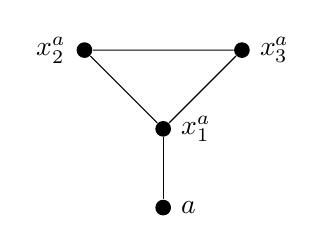
\begin{tikzpicture}
\tikzstyle{vertex}=[circle,fill=black,minimum size=1pt,inner sep=2pt]
\node[vertex,label=left:$x_2^a$] (2) at (0,0) {};
\node[vertex,label=right:$x^a_3$] (3) at (2,0) {};
\node[vertex,label=right:$x^a_1$] (1) at (1,-1) {};
\node[vertex,label=right:$a$] (a) at (1,-2) {};
\draw (2) -- (3) -- (1) -- (2);
\draw (a) -- (1);
\end{tikzpicture}
\end{center}

If \(a<b\), then \(G_A\) will have vertices \(y_1^{a,b},y_2^{a,b},y_3^{a,b}\) and
contain the subgraph

\begin{center}
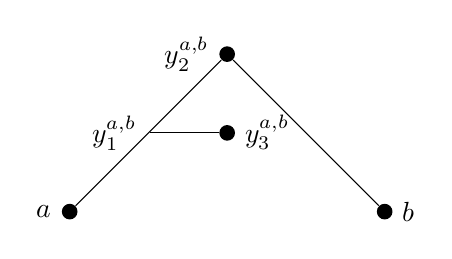
\begin{tikzpicture}
\tikzstyle{vertex}=[circle,fill=black,minimum size=1pt,inner sep=2pt]
\tikzstyle{empty}=[circle,fill=black,minimum size=1pt,inner sep=0]
\node[vertex,label=left:$y_2^{a,b}$] (2) at (2,2) {};
\node[label=left:$y_1^{a,b}$,inner sep=0] (1) at (1,1) {};
\node[vertex,label=right:$y_3^{a,b}$] (3) at (2,1) {};
\node[vertex,label=left:$a$] (a) at (0,0) {};
\node[vertex,label=right:$b$] (b) at (4,0) {};
\draw (a) -- (2);
\draw (1) -- (3);
\draw (2) -- (b);
\end{tikzpicture}
\end{center}


Let \(V_A=A\cup\{x_1^a,x_2^a,x_3^a:a\in A\}\cup\{y_1^{a,b},y_2^{a,b},y_3^{a,b}:a,b\in A\text{ and }a<b\}\), and let
\(R_A\) be the smallest symmetric relation containing all edges drawn above.

For example, if \(A\) is the three-element linear order \(a<b<c\), then \(G_A\) is
the graph

\begin{center}
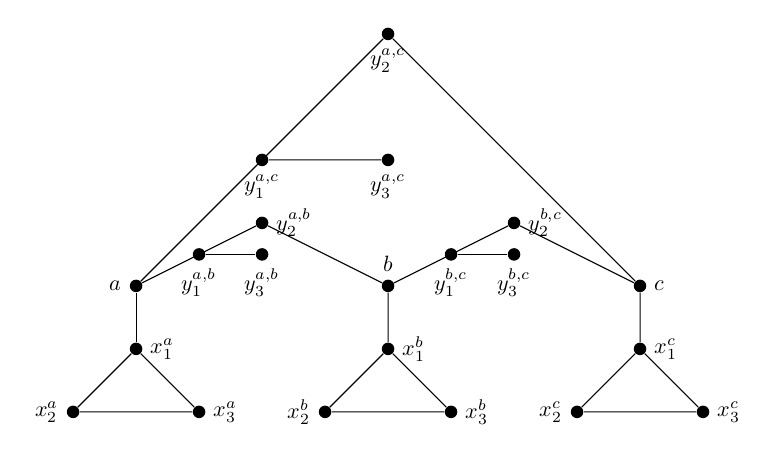
\begin{tikzpicture}[scale=0.8,transform shape]
\tikzstyle{vertex}=[circle,fill=black,minimum size=1pt,inner sep=2pt]
\tikzstyle{empty}=[circle,fill=black,minimum size=1pt,inner sep=0]
\node[vertex,label=left:$x_2^a$] (a2) at (0,0) {};
\node[vertex,label=left:$x_2^b$] (b2) at (4,0) {};
\node[vertex,label=left:$x_2^c$] (c2) at (8,0) {};
\node[vertex,label=right:$x_1^c$] (c1) at (9,1) {};
\node[vertex,label=right:$x_1^b$] (b1) at (5,1) {};
\node[vertex,label=right:$x_1^a$] (a1) at (1,1) {};
\node[vertex,label=right:$x_3^a$] (a3) at (2,0) {};
\node[vertex,label=right:$x_3^b$] (b3) at (6,0) {};
\node[vertex,label=right:$x_3^c$] (c3) at (10,0) {};
\node[vertex,label=left:$a$] (a) at (1,2) {};
\node[vertex,label=above:$b$] (b) at (5,2) {};
\node[vertex,label=right:$c$] (c) at (9,2) {};
\node[vertex,label=below:$y_1^{a,b}$] (ab1) at (2,2.5) {};
\node[vertex,label=below:$y_1^{b,c}$] (bc1) at (6,2.5) {};
\node[vertex,label=below:$y_3^{a,b}$] (ab3) at (3,2.5) {};
\node[vertex,label=right:$y_2^{a,b}$] (ab2) at (3,3) {};
\node[vertex,label=below:$y_3^{b,c}$] (bc3) at (7,2.5) {};
\node[vertex,label=right:$y_2^{b,c}$] (bc2) at (7,3) {};
\node[vertex,label=below:$y_3^{a,c}$] (ac3) at (5,4) {};
\node[vertex,label=below:$y_2^{a,c}$] (ac2) at (5,6) {};
\node[vertex,label=below:$y_1^{a,c}$] (ac1) at (3,4) {};
\draw (a2) -- (a1) -- (a3) -- (a2);
\draw (a1) -- (a);
\draw (b2) -- (b1) -- (b3) -- (b2);
\draw (b1) -- (b);
\draw (c2) -- (c1) -- (c3) -- (c2);
\draw (c1) -- (c);
\draw (a) -- (ac2);
\draw (ac2) -- (c);
\draw (a) -- (ab2);
\draw (ab1) -- (ab3);
\draw (ac1) -- (ac3);
\draw (bc1) -- (bc3);
\draw (b) -- (bc2);
\draw (b) -- (ab2);
\draw (c) -- (bc2);
\end{tikzpicture}
\end{center}

Let \(\call=\{R\}\) where \(R\) is a binary relation. Let \(\phi(x,u,v,w)\) be the
formula asserting that \(x,u,v,w\) are distinct, there are edges
\((x,u),(u,v),(v,w),(u,w)\) and these are the only edges involving \(u,v,w\).
\(G_A\vDash\phi(a,x_1^a,x_2^a,x_3^a)\) for all \(a\in A\).

\(\psi(x,y,u,v,w)\) asserts that \(x,y,u,v,w\) are distinct. \((x,u),(u,v),(u,w),(v,y)\)

Define \(\theta_i(z)\) as follows:
\begin{align*}
&\theta_0(z):=\exists u\exists v\exists w\;\phi(z,u,v,w)\\
&\theta_1(z):=\exists x\exists v\exists w\;\phi(x,z,v,w)\\
&\theta_2(z):=\exists u\exists u\exists w\;\phi(x,u,z,w)\\
&\theta_3(z):=\exists x\exists y\exists v\exists w\;\psi(x,y,z,v,w)\\
&\theta_4(z):=\exists x\exists y\exists u\exists w\;\psi(x,y,u,z,w)\\
&\theta_5(z):=\exists x\exists y\exists u\exists v\;\psi(x,y,u,v,z)\\
\end{align*}
If \(a,b\in A\) and \(a<b\), then
\begin{equation*}
G_A\vDash\theta_0(a)\wedge\theta_1(x^a_1)\wedge\theta_2(x^a_2)\wedge
\theta_2(x^a_3)
\end{equation*}
and 
\begin{equation*}
G_A\vDash\theta_3(y_1^{a,b})\wedge\theta_4(y_2^{a,b})\wedge\theta_5(
y_3^{a,b})
\end{equation*}
\begin{lemma}[]
If \((A,<)\) is a linear order, then for all vertices \(x\) in \(G\), there is a
unique \(i\le 5\) s.t. \(G_A\vDash\theta_i(x)\)
\end{lemma}

Let \(T\) be the \(\call\)-theory with the following axioms
\begin{enumerate}
\item \(R\) is symmetric and irreflexive
\item for all \(x\), exactly one \(\theta_i\) holds
\item if \(\theta_0(x)\) and \(\theta_0(y)\) then \(\neg R(x,y)\)
\item if \(\exists u\exists v\exists w\;\psi(x,y,u,v,w)\\\) then
\(\forall u_1\forall v_1\forall w_1\neg\psi(y,x,u_1,v_1,w_1)\)
\item if \(\exists u\exists v\exists w\;\psi(x,y,u,v,w)\) and 
\(\exists u\exists v\exists w\;\psi(y,z,u,v,w)\) then\par
\(\exists u\exists v\exists w\;\psi(x,z,u,v,w)\)
\item if \(\theta_0(x)\) and \(\theta_0(y)\), then either \(x=y\) or 
\(\exists u\exists v\exists w\;\psi(x,y,u,v,w)\) or
\(\exists u\exists v\exists w\;\psi(y,x,u,v,w)\)
\item if \(\phi(x,u,v,w)\wedge\phi(x,u',v',w')\), then
\(u=u',v=v',w=w'\)
\item if \(\psi(x,y,u,v,w)\wedge\psi(x,y,u',v',w')\), then
\(u'=u,v=v',w=w'\)
\end{enumerate}


If \((A,<)\) is a linear order, then \(G_A\vDash T\)

Suppose \(G\vDash T\). Let \(X_G=\{x\in G:G\vDash\theta_0(x)\}\)

\begin{lemma}[]
If \((A,<)\) is a linear order, then \((X_{G_A},<_{G_A})\cong(A,<)\). Moreover,
\(G_{X_G}\cong G\) for all \(G\vDash T\)
\end{lemma}

\begin{definition}[]
An \(\call_0\)-structure \(\caln\) is \textbf{interpretable} in an
\(\call\)-structure \(M\) if there is a definable \(X\subseteq M^n\), a definable
equivalence relation \(E\) on \(X\), and for each symbol of \(\call_0\) we can find
definable \(E\)-invariant sets on X s.t. \(X/E\) with the induced structure is
isomorphic to \(\caln\)
\end{definition}
\subsection{Answers to Exercises}
\label{sec:orgcaac325}
\begin{exercise}
\begin{enumerate}
\item transform \(\psi\) to CNF
\item prenex normal form
\end{enumerate}
\end{exercise}
\begin{exercise}
\begin{enumerate}
\item 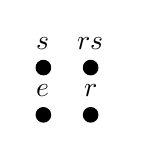
\begin{tikzpicture}[scale=0.6]
\tikzstyle{vertex}=[circle,fill=black,minimum size=1pt,inner sep=2pt]
\node[vertex,label=above:$s$] (1) at (0,1) {};
\node[vertex,label=above:$e$] (0) at (0,0) {};
\node[vertex,label=above:$r$] (2) at (1,0) {};
\node[vertex,label=above:$rs$] (3) at (1,1) {};
\end{tikzpicture}
\item enumerate \(\calm\)'s functions, relations and constants
\end{enumerate}
\end{exercise}
\begin{exercise}
\footnote{\href{https://math.stackexchange.com/questions/1170953/let-alpha-be-any-cardinal-there-are-at-most-2-alpha-cup-mathscrl}{stackexchange}}
Note that every \(\call\)-structure \(\calm\) of size \(\kappa\) is isomorphic to an
\(\call\)-structure with domain \(\kappa\). For each relation symbols, we have \(2^\kappa\)
options. If the language has size \(\lambda\), this is at most 
\((2^\kappa)^\lambda=2^{\kappa\cdot\lambda}=2^{\max(\lambda,\kappa)}\)
\end{exercise}

\begin{exercise}
\begin{align*}
T\vDash\phi&\Leftrightarrow\forall \calm\;\calm\vDash T\to\calm\vDash\phi\\
&\Leftrightarrow\forall \calm\;\calm\vDash T'\to\calm\vDash\phi\\
&\Leftrightarrow T'\vDash\phi
\end{align*}
\end{exercise}
\begin{exercise}
Follow the definition
\end{exercise}

\begin{exercise}
Since there is no model \(\calm\) s.t. \(\calm\vDash T\). It's true that 
\(T\vDash \phi\)
\end{exercise}

\begin{exercise}
\begin{enumerate}
\item Suppose \(\calm\vDash\phi\), then \(E^{\calm}\) is an equivalent relation and
each equivalence class's cardinality is 2
\item follows from number theory
\item \cite{DBLP:journals/bsl/DurandJMM12}
\end{enumerate}
\end{exercise}

\begin{exercise}
TBD
\end{exercise}

\begin{exercise}
\(G(f)=\{(\bar{x},\bar{y})\in M^{n+m}\mid\phi(\bar{x},\bar{y})\}\) and 
\(G(g)=\{(\bar{y},\bar{z})\in M^{m+l}\mid\psi(\bar{y},\bar{z})\}\). Hence
\(G(g\circ f)=\{(\bar{x},\bar{z})\in M^{n+l}\mid \phi(\bar{x},\bar{y})
   \wedge \psi(\bar{y},\bar{z})\}\)
\end{exercise}

\begin{exercise}
\(\phi(\bar{a},b)\) really defines a function and since 
\(\phi(\bar{a},y)\to y=b\)
\end{exercise}

\section{Basic Techniques}
\label{sec:orgf8c45c3}
\subsection{The Compactness Theorem}
\label{sec:org4f33416}

Some points of proofs
\begin{itemize}
\item Proofs are finite
\item (Soundness) If \(T\vdash\phi\), then \(T\vDash\phi\)
\item If \(T\) is a finite set of sentences, then there is an algorithm that,
when given a sequence of \(\call\)-formulas \(\sigma\) and an \(\call\)-sentence \(\phi\),
will decide whether \(\sigma\) is a proof of \(\phi\) from \(T\)
\end{itemize}

\index{recursive}
A language \(\call\) is \textbf{recursive} if there is an algorithm that decides
whether a sequence of symbols is an \(\call\)-formula. An \(\call\)-theory
\(T\) is \textbf{recursive} if there is an algorithm that when given an
\(\call\)-sentence \(\phi\) as input, decides whether \(\phi\in T\)

\begin{proposition}[]
\label{prop2.1.1}
If \(\call\) is a recursive language and \(T\) is a recursive \(\call\)-theory,
then \(\{\phi:T\vdash\phi\}\) is recursively enumerable; that is, there is an
algorithm that when given \(\phi\) as input will halt accepting if \(T\vdash\phi\)
and not halt if \(T\not\vdash\phi\)
\end{proposition}
\begin{proof}
There is \(\sigma_0,\sigma_1,\dots\) a computable listing of all finite
sequence of \(\call\)-formulas. At stage \(i\), we check to see whether
\(\sigma_i\) is a proof of \(\psi\) from \(T\). If it is, then halt.
\end{proof}

\begin{theorem}[Gödel's Completeness Theorem]
Let \(T\) be an \(\call\)-theory and \(\phi\) an \(\call\)-sentence, then
\(T\vDash\phi\) if and only if \(T\vdash \phi\)
\end{theorem}

We say that an \(\call\)-theory \(T\) is \textbf{inconsistent} if
\(T\vdash(\phi\wedge\neg\phi)\) for some sentence \(\phi\).

\begin{corollary}[]
\(T\) is consistent if and only if \(T\) is satisfiable
\end{corollary}

\begin{proof}
Supose that \(T\) is not satisfiable, then every model of \(T\) is a model of
\(\phi\wedge\neg\phi\). Thus by the Completeness theorem
\(T\vdash(\phi\wedge\neg\phi)\) 
\end{proof}


\begin{theorem}[Compactness Theorem]
\(T\) is satisfiable if and only if every finite subset of \(T\) is satisfiable
\end{theorem}

\begin{proof}
If \(T\) is not satisfiable, then \(T\) is inconsistent. Let \(\sigma\) be a proof of
a contradiction from  \(T\). Because \(\sigma\) is finite, only finitely many
assumptions from \(T\) are used in the proof. Thus there is a finite
\(T_0\subseteq T\) s.t. \(\sigma\) is a proof of a contradiction from \(T_0\)
\end{proof}

\subsubsection{Henkin Constructions}
\label{sec:org44bb2cf}
\index{finitely satisfiable}
A theory \(T\) is \textbf{finitely satisfiable} if every finite subset of \(T\) is
satisfiable. We will show that every finitely satisfiable theory \(T\) is
satisfiable.

\begin{definition}[]
We say that an \(\call\)-theory \(T\) has the \textbf{witness property} if whenever
\(\phi(v)\) is an \(\call\)-formula with one free variable \(v\), then there is
a constant symbol \(c\in\call\) s.t. \(T\vdash(\exists v\phi(v))\to\phi(c)\in T\)

An \(\call\)-theory \(T\) is \textbf{maximal} if for all \(\phi\) either \(\phi\in T\) or
\(\neg\phi\in T\)
\end{definition}

\begin{lemma}[]
\label{lemma2.1.6}
Suppose \(T\) is a maximal and finitely satisfiable \(\call\)-theory. If
\(\Delta\subseteq T\) is finite and \(\Delta\vDash\psi\), then \(\psi\in T\)
\end{lemma}

\begin{proof}
If \(\psi\not\in T\), then \(\neg\psi\in T\) but \(\Delta\cup\{\psi\}\) is
unsatisfiable 
\end{proof}

\begin{lemma}[]
\label{lemma2.1.7}
Suppose that \(T\) is a maximal and finitely satisfiable \(\call\)-theory with
the witness property. Then \(T\) has a model. In fact, if \(\kappa\) is a cardinal
and \(\call\) has at most \(\kappa\) constant symbols, then there is
\(\calm\vDash T\) with \(\abs{\calm}\le\kappa\)
\end{lemma}

\begin{proof}
Let \(\calc\) be the set of constant symbols of \(\call\). For \(c,d\in\calc\),
we say \(c\sim d\) if \(c=d\in T\)

\textbf{Claim 1} \(\sim\) is an equivalence relation. 

The universe of our model will be \(M=\calc/\sim\). Clearly
\(\abs{M}\le\kappa\). We let \(c^*\) denote the equivalence class of \(c\) and
interprete \(c\) as its equivalence class, that is, \(c^{\calm}=c^*\)

Suppose that \(R\) is an \(n\)-ary relation symbol of \(\call\)

\textbf{Claim 2} Suppose that \(c_1,\dots,c_n,d_1,\dots,d_n\in\calc\) and \(c_i\sim d_i\)
for \(i=1,\dots,n\), then \(R(\bar{c})\) if and only if \(R(\bar{d})\)

By Lemma \ref{lemma2.1.6}, if one of \(R(\bar{c})\) and \(R(\bar{d})\) is
in \(T\), then both are in \(T\)


\begin{equation*}
R^{\calm}=\{(c_1^*,\dots,c_n^*):R(c_1,\dots,c_n)\in T\}
\end{equation*}
Suppose that \(f\) is an \(n\)-ary function symbol of \(\call\) and
\(c_1,\dots,c_n\in\calc\). Because  \(\underline{\emptyset\vDash\exists
    vf(c_1,\dots,c_n)=v}\), and \(T\) has the witness property, then there is
\(c_{n+1}\in\calc\) s.t. \(f(c_1,\dots,c_n)=c_{n+1}\in T\). As above, if
\(d_i\sim c_i\) for \(i=1,\dots,n+1\), then \(f(d_1,\dots,d_n)=d_{n+1}\in T\).
Thus we get a well-defined function \(f^{\calm}:M^n\to M\) by
\begin{equation*}
f^{\calm}(c_1^*,\dots,c_n^*)=d^*\text{ if and only if }f(c_1,\dots,c_n)=d\in T
\end{equation*}

\textbf{Claim 3} Suppose that \(t\) is a term using free variables from
\(v_1,\dots,v_n\). If \(c_1,\dots,c_n,d\in\calc\), then \(t(c_1,\dots,c_n)=d\in
    T\) if and only if \(t^{\calm}(c_1^*,\dots,c_n^*)=d^*\)

(\(\Rightarrow\)) If \(t\) is a constant symbol, then \(c=d\in T\) and
\(c^{\calm}=c^*=d^*\)

If \(t\) is the variable \(v_i\), then \(c_i=d\in T\) and 
\(t^{\calm}(c_1^*,\dots,c_n^*)=c_i^*=d^*\)

Suppose that the claim is true for \(t_1,\dots,t_m\) and \(t\) is
\(f(t_1,\dots,t_m)\). Using the witness property and Lemma \ref{lemma2.1.6},
we can find \(d,d_1,\dots,d_n\in\calc\) s.t. \(t_i(c_1,\dots,c_n)=d_i\in T\)
for \(i\le m\) and \(f(d_1,\dots,d_m)=d\in T\). By our induction hypothesis, 
\(t_i^{\calm}(c_1^*,\dots,c_n^*)=d_i^*\) and
\(f^{\calm}(d_1^*,\dots,d_m^*)=d^*\). Thus \(t^{\calm}(c_1^*,\dots,c_n^*)=d^*\)

(\(\Leftarrow\)) Suppose \(t^{\calm}(c_1^*,\dots,c_n^*)=d^*\). By the witness
property, there is a \(e\in\calc\) s.t. \(t(c_1,\dots,c_n)=e\in T\). Using the
\((\Rightarrow)\) direction of the proof, \(t^{\calm}(c_1^*,\dots,c_n^*)=e^*\).
Thus \(e^*=d^*\) and \(e=d\in T\)


\textbf{Claim 4} For all \(\call\)-formulas \(\phi(v_1,\dots,v_n)\) and
\(c_1,\dots,c_n\in\calc\), \(\calm\vDash\phi(\bar{c}^*)\) if and only if
\(\phi(\bar{c})\in T\)

Suppose that \(\phi\) is \(t_1=t_2\). By Lemma \ref{lemma2.1.6} and the
witness property, we can find \(d_1\) and \(d_2\) s.t. 
\(t_1(\bar{c})=d_1,t_2(\bar{c})=d_2\in T\). By Claim 3,
\(t_i^{\calm}(\bar{c}^*)=d_i^*\). Then
\begin{align*}
\calm\vDash\phi(\bar{c}^*)&\Leftrightarrow d_1^*=d_2^*\\
&\Leftrightarrow d_1=d_2\in T\\
&\Leftrightarrow t_1(\bar{c})=t_2(\bar{c})\in T
\end{align*}

Suppose that \(\phi\) is \(R(t_1,\dots,t_m)\). There are \(d_1,\dots,d_m\in\calc\)
s.t. \(t_i(\bar{c})=d_i\in T\). Thus
\begin{align*}
\calm\vDash\phi(\bar{c}^*)&\Leftrightarrow \bar{d}^*\in R^{\calm}\\
&\Leftrightarrow R(\bar{d})\in T\\
&\Leftrightarrow\phi(\bar{c})\in T
\end{align*}

Suppose that the claim is true for \(\phi\). If
\(\calm\vDash\neg\phi(\bar{c}^*)\), then
\(\calm\not\vDash\phi(\bar{c}^*)\). By the inductive hypothesis,
\(\phi(\bar{c})\not\in T\). Thus by maximality, \(\neg\phi(\bar{c})\in T\). On
the other hand, if \(\neg\phi(\bar{c})\in T\), then because \(T\) is finitely
satisfiable, \(\phi(\bar{c})\not\in T\). Thus, by induction,
\(\calm\not\vDash\phi(\bar{c}^*)\).
\end{proof}

\begin{lemma}[]
\label{lemma2.1.8}
Let \(T\) be a finitely satisfiable \(\call\)-theory. There is a language
\(\call^*\supseteq\call\) and \(T^*\supseteq T\) a finitely satisfiable
\(\call^*\)-theory s.t. any \(\call^*\)-theory extending \(T^*\) has the
witness property. We can choose \(\call^*\) s.t.
\(\abs{\call^*}=\abs{\call}+\aleph_0\) 
\end{lemma}

\begin{proof}
We first show that there is a language \(\call_1\supseteq\call\) and a
finitely satisfiable \(\call_1\)-theory \(\call_1\supseteq T\) s.t. for any
\(\call\)-formula \(\phi(v)\) there is an \(\call_1\)-constant symbol \(c\) s.t.
\(T_1\vDash(\exists v\phi(v))\to\phi(c)\). For each \(\call\)-formula
\(\phi(v)\), let \(c_\phi\) be a new constant symbol and let
\(\call_1=\call\cup\{c_\phi:\phi(v)\text{ an }\call\text{-formula}\}\). For
each \(\call\)-formula \(\phi(v)\), let \(\Theta_\phi\) be the
\(\call_1\)-sentence
\((\exists v\phi(v))\to\phi(c_\phi)\). Let
\(T_1=T\cup\{\Theta_\phi:\phi(v)\text{ an }\call\text{-formula}\}\)

\textbf{Claim} \(T_1\) is finitely satisfiable

Suppose that \(\Delta\) is a finite subset of \(T_1\). Then
\(\Delta=\Delta_0\cup\{\Theta_{\phi_1},\dots, \Theta_{\phi_n}\}\) where
\(\Delta_0\) is a finite subset of \(T\) and there is \(\calm\vDash\Delta_0\). We
will make \(\calm\) into an
\(\call\cup\{c_{\phi_1},\dots,c_{\phi_n}\}\)-structure \(\calm'\). If
\(\calm\vDash\exists v\phi(v)\), choose \(a_i\) some element of \(M\) s.t.
\(\calm\vDash\phi(a_i)\) and let \(c_{\phi_i}^{\calm'}=a_i\). Otherwise, let
\(c_{\phi_i}^{\calm'}\) be any element of \(\calm\). Clearly
\(\calm'\vDash\Theta_{\phi_i}\) for \(i\le n\). Thus \(T_1\) is finitely
satisfiable.

We now iterate the construction above to build a sequence of languages
\(\call\subseteq\call_1\subseteq\call_2\subseteq\dots\) and a sequence of
finitely satisfiable \(\call_i\)-theories \(T\subseteq T_1\subseteq
    T_2\subseteq\dots\) s.t. if \(\phi(v)\) is an \(\call_i\)-formula then there is
a constant symbol \(c\in\call_{i+1}\) s.t. \(T_{i+1}\vDash(\exists
    v\phi(v))\to\phi(c)\)

Let \(\call^*=\bigcup\call_i\) and \(T^*=\bigcup T_i\). 
If \(\abs{\call_i}\) is the number of relation, function and constant
symbols in \(\call_i\), then there are at most \(\abs{\call_i}+\aleph_0\)
formulas in \(\call_i\).
Thus by induction,
\(\abs{\call^*}=\abs{\call}+\aleph_0\) 
\end{proof}

\begin{lemma}[]
\label{2.1.9}
Suppose that \(T\) is a finitely satisfiable \(\call\)-theory and \(\phi\) is an
\(\call\)-sentence, then either \(T\cup\{\phi\}\) or \(T\cup\{\neg\phi\}\) is
finitely satisfiable
\end{lemma}

\begin{corollary}[]
\label{cor2.1.10}
If \(T\) is a finitely satisfiable \(\call\)-theory, then there is a maximal
finitely satisfiable \(\call\)-theory \(T'\supseteq T\)
\end{corollary}
\begin{proof}
Let \(I\) be the set of all finitely satisfiable \(\call\)-theory containing
\(T\). We partially order \(I\) by inclusion. If \(C\subseteq I\) is a chain, let
\(T_C=\bigcup\{\Sigma:\Sigma\in C\}\). If \(\Delta\) is a finite subset of
\(T_C\), then there is a \(\Sigma\in C\) s.t. \(\Delta\subseteq\Sigma\), so \(T_C\)
is finitely satisfiable and \(T_C\supseteq\Sigma\) for all \(\Sigma\in C\). Thus
every chain in \(I\) has an upper bound, and we can apply Zorn's lemma to find
a \(T'\in I\) maximal w.r.t. the partial order.
\end{proof}


\begin{theorem}[strengthening of Compactness Theorem]
\label{thm2.1.11}
If \(T\) is a finitely satisfiable \(\call\)-theory and \(\kappa\) is an infinite
cardinal with \(\kappa\ge\abs{\call}\), then there is a model of \(T\) of
cardinality at most \(\kappa\)
\end{theorem}

\begin{proof}
By Lemma \ref{lemma2.1.8}, we can find \(\call^*\supseteq\call\) and 
\(T^*\supseteq T\) a finitely satisfiable \(\call^*\)-theory s.t. any
\(\call^*\)-theory extending \(T^*\) has the witness property and the
cardinality of \(\call^*\) is at most \(\kappa\). By Corollary \ref{cor2.1.10}, we can
find a maximal finitely satisfiable \(\call^*\)-theory 
\(T'\supseteq T^*\). Because \(T'\) has the witness property, Lemma
\ref{lemma2.1.7} ensures that there is \(\calm\vDash T\) with \(\abs{M}\le\kappa\)
\end{proof}

\begin{proposition}[]
Let \(\call=\{\cdot,+,<,0,1\}\) and let \(\Th(\N)\) be the full \(\call\)-theory
of the natural numbers. There is \(\calm\vDash\Th(\N)\) and \(a\in M\) s.t. \(a\)
is larger than every natural number
\end{proposition}

\begin{proof}
Let \(\call^*=\call\cup\{c\}\) where \(c\) is a new constant symbol and let
\begin{equation*}
T=\Th(\N)\cup\{\underbrace{1+1+\dots+1}_{n\text{-times}}<c:\text{for }n=1,2,\dots\} 
\end{equation*}
If \(\Delta\) is a finite subset of \(T\) we can make \(\N\) a model of \(\Delta\) by
interpreting \(c\) as a suitably large natural number. Thus \(T\) is finitely
satisfiable and there is \(\calm\vDash T\).
\end{proof}
\begin{lemma}[]
\label{lemma2.1.14}
If \(T\vDash\phi\), then \(\Delta\vDash T\) for some finite \(\Delta\subseteq T\)
\end{lemma}
\begin{proof}
Suppose not. Let \(\Delta\subseteq T\) be finite. Because
\(\Delta\not\vDash\phi\), \(\Delta\cup\{\neg\phi\}\) is satisfiable. Thus
\(T\cup\{\neg\phi\}\) is finitely satisfiable and by the compactness theorem,
\(T\not\vDash\phi\) 
\end{proof}



\subsection{Complete Theories}
\label{sec:org44049ce}
\index{complete}
\begin{definition}[]
An \(\call\)-theory \(T\) is called \textbf{complete} if for any \(\call\)-sentence \(\phi\)
either \(T\vDash\phi\) or \(T\vDash\neg\phi\)
\end{definition}

For \(\calm\) an \(\call\)-structure, then the full theory
\begin{equation*}
\Th(\calm)=\{\phi:\phi\text{ is an }\call\text{-sentence and }
\calm\vDash\phi\}
\end{equation*}
is a complete theory.

\begin{proposition}[]
\label{prop2.2.2}
Let \(T\) be an \(\call\)-theory with infinite models. If \(\kappa\) is an infinite
cardinal and \(\kappa\ge\abs{\call}\), then there is a model of \(T\) of
cardinality \(\kappa\)
\end{proposition}

\begin{proof}
Let \(\call^*=\call\cup\{c_\alpha:\alpha<\kappa\}\), where each \(c_\alpha\) is
new constant symbol, and let \(T^*\) be the \(\call^*\)-theory
\(T\cup\{c_\alpha\neq c_\beta:\alpha,\beta<\kappa,\alpha\neq\beta\}\). Clearly
if \(\calm\vDash T^*\), then \(\calm\) is a model of \(T\) of cardinality at least
\(\kappa\).
Thus by Theorem \ref{thm2.1.11}, it suffices to show that \(T^*\) is finitely
satisfiable. But if \(\Delta\subseteq T^*\) is finite, then \(\Delta\subseteq
   T\cup\{c_\alpha\neq c_\beta:\alpha\neq\beta,\alpha,\beta\in I\}\), where \(I\)
is a finite subset of \(\kappa\). Let \(\calm\) be an infinite model of \(T\). We can
interpret the symbols \(\{c_\alpha:\alpha\in I\}\) as \(\abs{I}\) distinct
elements of \(M\). Because \(\calm\vDash\Delta\), \(T^*\) is finitely satisfiable.
\end{proof}

\begin{definition}[]
Let \(\kappa\) be an infinite cardinal and let \(T\) be a theory with models of
size \(\kappa\). We say that \(T\) is \textbf{\(\kappa\)-categorical} if any two models of
\(T\) of cardinality \(\kappa\) are isomorphic.
\end{definition}

Let \(\call=\{+,0\}\) be the language of additive groups and let \(T\) be the
\(\call\)-theory of torsion-free divisible Abelian groups. The axioms of \(T\)
are the axioms for Abelian groups together with the axioms
\begin{gather*}
\forall x(x\neq 0\to\underbrace{x+\dots+x}_{n\text{-times}}\neq 0)\\
\forall y\exists x\underbrace{x+\dots+x}_{n\text{-times}}=y
\end{gather*}
for \(n=1,2,\dots\)


\begin{proposition}[]
\label{prop2.2.4}
The theory of torsion-free divisible Abelian groups is \(\kappa\)-categorical for
all \(\kappa>\aleph_0\)
\end{proposition}

\begin{proof}
We first argue that models of \(T\) are essentially vector spaces over the
field of rational numbers \(\Q\). If \(V\) is any vector space over \(\Q\), then
the underlying additive group \(V\) is a model of \(T\). 
Check \href{https://math.stackexchange.com/questions/1550900/necessary-and-sufficient-conditions-for-an-abelian-group-to-be-a-vector-space-ov/1550954}{StackExchange}.
On the other hand, if
\(G\vDash T\), \(g\in G\) and \(n\in\N\) with \(g>0\), we can find 
\(h\in G\) s.t. \(nh=g\). If \(nk=g\), then \(n(h-k)=0\). Because \(G\) is
torsion-free there is a unique \(h\in G\) s.t. \(nh=g\). We call this element 
\(g/n\). We can view \(G\) as a \(\Q\)-vector space under the action
\(\frac{m}{n}g=m(g/n)\)

Two \(\Q\)-vector spaces are isomorphic if and only if they have the same
dimension. Thus the model of \(T\) are determined up to isomorphism by their
dimension. If \(G\) has dimension \(\lambda\), then \(\abs{G}=\lambda+\aleph_0\). If \(\kappa\)
is uncountable and \(G\) has cardinality \(\kappa\), then \(G\) has dimension \(\kappa\). Thus for
\(\kappa>\aleph_0\) any two models of \(T\) of cardinality \(\kappa\) are isomorphic
\end{proof}

\begin{lemma}[]
\label{lemmamy1}
Field of uncountable cardinality \(\kappa\) has transcendence degree \(\kappa\)
\footnote{\href{https://proofwiki.org/wiki/Field\_of\_Uncountable\_Cardinality\_K\_has\_Transcendence\_Degree\_K}{proofwiki}}
\end{lemma}

\begin{proof}
We prove the theorem for fields with characteristic \(p=0\). 

Since each characteristic 0 field contains a copy of \(\Q\) as its prime
field, we can view \(F\) as a field extension over \(\Q\). We will show that
\(F\) has a subset of cardinality \(\kappa\) which is algebraically independent over
\(\Q\).

We build the claimed subset of \(F\) by transfinite induction and implicit use
of the axiom of choice.

Let \(S_0=\emptyset\)

Let \(S_1\) be a singleton containing some element of \(F\) which is not
algebraic over \(\Q\). This is possible since algebraic numbers are countable

Define \(S_{\alpha+1}\) to be \(S_\alpha\) together with an element of \(F\)
which is not a root of any non-trivial polynomial with coefficients in 
\(\Q\cup S_\alpha\) since there are only 
\(\abs{\Q\cup S_\alpha}=\aleph_0+\abs{\alpha}<\kappa\) polynomials

Define \(S_\beta=\displaystyle\bigcup_{\alpha<\beta}S_\alpha\)

Let \(P(x_1,\dots,x_n)\) be a non-trivial polynomial with coefficients in
\(\Q\) and elements \(a_1,\dots,a_n\) in \(F\). W.L.O.G., it is assumed that
\(a_n\) was added at an ordinal \(\alpha+1\) later than the other elements.
Then \(P(a_1,\dots,a_{n-1},x_n)\) is a polynomial with coefficients in 
\(\Q\cup S_\alpha\). Hence \(P(a_1,\dots,a_n)\neq0\).
\end{proof}

\begin{proposition}[]
\label{prop2.2.5}
\(\ACF_p\) is \(\kappa\)-categorical for all uncountable cardinals \(\kappa\)
\end{proposition}

\begin{proof}
Two algebraically closed fields are isomorphic if and only if they have the
same characteristic and transcendence degree. See
\url{AdvancedModernAlgebra.org}. By Lemma
\ref{lemmamy1}, an algebraically closed field of transcendence degree \(\lambda\) has
cardinality \(\lambda+\aleph_0\).
\end{proof}

\begin{theorem}[Vaught's Test]
\label{thm2.2.6}
Let \(T\) be a satisfiable theory with no finite models that is
\(\kappa\)-categorical for some infinite cardinal \(\kappa\ge\abs{\call}\). Then
\(T\) is complete
\end{theorem}

\begin{proof}
Suppose \(T\) is not complete. Then there is a sentence \(\phi\) s.t. 
\(T\not\vDash\phi\) and \(T\not\vDash\neg\phi\). Because
\(T\not\vDash\psi\) if and only if \(T\cup\{\neg\psi\}\) is satisfiable, the
theories \(T_0=T\cup\{\phi\}\) and \(T_1=T\cup\{\neg\phi\}\) are satisfiable.
Because \(T\) has no finite models, both \(T_0\) and \(T_1\) have infinite
models. By Proposition \ref{prop2.2.2} we can find \(\calm_0\) and
\(\calm_1\) of cardinality \(\kappa\) with \(\calm_i\vDash T_i\). Because \(\calm_0\)
and \(\calm_1\) disagree about \(\phi\), they are not elementarily equivalent, and
hence by Theorem \ref{thm1.1.10}, nonisomorphic. 
\end{proof}

\begin{definition}[]
We say that an \(\call\)-theory \(T\) is \textbf{decidable} if there is an algorithm
that when given an \(\call\)-sentence \(\phi\) as input decides whether \(T\vDash\phi\)
\end{definition}

\begin{lemma}[]
\label{lemma2.2.8}
Let \(T\) be a recursive complete satisfiable theory in a recursive language
\(\call\). Then \(T\) is decidable
\end{lemma}

\begin{proof}
Because \(T\) is satisfiable \(A=\{\phi:T\vDash\phi\}\) and
\(B=\{\phi:T\vDash\neg\phi\}\) are disjoint. Because \(T\) is consistent 
\(A\cup B\) is the set of all \(\call\)-sentences. By the Completeness
Theorem, \(A=\{\phi:T\vdash\phi\}\) and \(B=\{\phi:T\vdash\neg\phi\}\). By
Proposition \ref{prop2.1.1} \(A\) and \(B\) are recursively enumerable. But any
recursively enumerable set with a recursively enumerable complement is
recursive. 
\end{proof}

\begin{corollary}[]
For \(p=0\) or \(p\) prime, \(ACF_p\) is decidable. In particular, \(\Th(\C)\),
the first-order theory  of the field of complex numbers, is decidable
\end{corollary}

\begin{corollary}[]
Let \(\phi\) be a sentence in the language of rings. The following are equivalent
\begin{enumerate}
\item \(\phi\) is true in the complex number
\item \(\phi\) is true in every algebraically closed field of characteristic zero
\item \(\phi\) is true in some algebraically closed field of characteristic zero
\item There are arbitrarily large primes \(p\) s.t. \(\phi\) is true in some
algebraically closed field of characteristic \(p\)
\item There is an \(m\) s.t. for all \(p>m\), \(\phi\) is true in all algebraically
closed fields of characteristic \(p\)
\end{enumerate}
\end{corollary}

\begin{proof}
By Proposition \ref{prop2.2.5} and Vaught's Test, \(\ACF_p\) is complete.

\((2)\to(5)\). Suppose that \(\ACF_0\vDash\phi\). By Lemma \ref{lemma2.1.14},
there is a finite \(\Delta\subseteq\ACF_0\) s.t. \(\Delta\vDash\phi\). Thus
if we choose \(p\) large enough, then \(\ACF_p\vDash\Delta\).

\((4)\to(2)\). Suppose \(\ACF_0\not\vDash\phi\). Because \(\ACF_0\) is
complete, \(\ACF_0\vDash\neg\phi\).
\end{proof}

\subsection{Up and Down}
\label{sec:orgbec03d5}


\begin{definition}[]
If \(\calm\) and \(\caln\) are \(\call\)-structures, then an
\(\call\)-embedding \(j:\calm\to\caln\) is called an \textbf{elementary embedding} if
\begin{equation*}
\calm\vDash\phi(a_1,\dots,a_n)\leftrightarrow\caln\vDash\phi(j(a_1),\dots,j(a_n))
\end{equation*}
for all \(\call\)-formulas \(\phi(v_1,\dots,v_n)\) and all \(a_1,\dots,a_n\in
   M\)

If \(\calm\) is a substructure of \(\caln\), we say that it is an \textbf{elementary
substructure} and write \(\calm\prec\caln\) if the inclusion map is elementary.
\(\caln\) is an \textbf{elementary extension} of \(\calm\)
\end{definition}

\begin{definition}[]
\(\calm\) is an \(\call\)-structure. Let \(\call_M\) be the language where we
add to \(\call\) constant symbols \(m\) for each element of \(M\). The \textbf{atomic
diagram} of \(\calm\) is
\(\{\phi(m_1,\dots,m_n):\phi\) is either an atomic \(\call\)-formula or the negation of an atomic
\(\call\)-formula and
\(\calm\vDash\phi(m_1,\dots.m_n)\}\).
The \textbf{elementary diagram} of \(\calm\) is 
\begin{equation*}
\{\phi(m_1,\dots,m_n):\calm\vDash\phi(m_1,\dots,m_n),\phi\text{ an 
\(\call\)-formula}\}
\end{equation*}

We let \(\Diag(\calm)\) and \(\Diag_{\el}(\calm)\) denote the atomic and
elementary diagrams of \(\calm\)
\end{definition}

\begin{lemma}[]
\label{lemma2.3.3}
\begin{enumerate}
\item Suppose that \(\caln\) is an \(\call_M\)-structure and
\(\caln\vDash\Diag(\calm)\), then viewing \(\caln\) as an
\(\call\)-structure, there is an \(\call\)-embedding of \(\calm\) into \(\caln\)
\item If \(\caln\vDash\Diag_{\el}(\calm)\), then there is an elementary
embedding of \(\calm\) into \(\caln\)
\end{enumerate}
\end{lemma}

\begin{proof}
\begin{enumerate}
\item Let \(j:M\to N\) by \(j(m)=m^{\caln}\). If \(m_1\neq m_2\in\Diag(\calm)\);
thus \(j(m_1)\neq j(m_2)\) so \(j\) is an embedding. If \(f\) is a function
symbols of \(\call\) and \(f^{\calm}(m_1,\dots,m_n)=m_{n+1}\), then
\(f(m_1,\dots,m_n)=m_{n+1}\) is a formula in \(\Diag(\calm)\) and 
\(f^{\caln}(j(m_1),\dots,j(m_n))=j(m_{n+1})\). If \(R\) is a relation symbol
and \(\bar{m}\in R^{\calm}\), then \(R(m_1,\dots,m_n)\in\Diag(\calm)\) and 
\((j(m_1),\dots,j(m_{n}))\in R^{\caln}\). Hence \(j\) is an
\(\call\)-embedding
\item \(j\) is elementary.
\end{enumerate}
\end{proof}

\begin{theorem}[Upward Löwenheim–Skolem Theorem]
Let \(\calm\) be an infinite \(\call\)-structure and \(\kappa\) be an infinite
cardinal \(\kappa\ge\abs{\calm}+\abs{\call}\). Then, there is \(\caln\) an
\(\call\)-structure of cardinality \(\kappa\) and \(j:\calm\to\caln\) is elementary
\end{theorem}

\begin{proof}
Because \(\calm\vDash\Diag_{\el}(\calm)\), \(\Diag_{\el}(\calm)\) is
satisfiable. By Theorem \ref{thm2.1.11}, there is
\(\caln\vDash\Diag_{\el}(\calm)\) of cardinality \(\kappa\). By Lemma \ref{lemma2.3.3},
there is an elementary \(j:\calm\to\caln\)
\end{proof}

\begin{proposition}[Tarski-Vaught Test]
\label{prop2.3.5}
Suppose that \(\calm\) is a substructure of \(\caln\). Then \(\calm\) is an
elementary substructure if and only if, for any formula \(\phi(v,\bar{w})\) and 
\(\bar{a}\in M\), if there is \(b\in N\) s.t.
\(\caln\vDash\phi(b,\bar{a})\), then there is \(c\in M\) s.t.
\(\caln\vDash\phi(c,\bar{a})\) 
\end{proposition}

\begin{proof}
We need to show that for all \(\bar{a}\in M\) and all \(\call\)-formulas
\(\psi(\bar{v})\)
\begin{equation*}
\calm\vDash\psi(\bar{a})\Leftrightarrow\caln\vDash\psi(\bar{a})
\end{equation*}

In Proposition \ref{prop1.1.8}, we showed that if \(\phi(\bar{v})\) is quantifier
free then \(\calm\vDash\phi(\bar{a})\) if and only if \(\phi(\bar{a})\)
\end{proof}

We say that an \(\call\)-theory \(T\) has \textbf{built-in Skolem functions} if for all
\(\call\)-formulas \(\phi(v,w_1,\dots,w_n)\) there is a function symbol \(f\) s.t.
\(T\vDash\forall\bar{w}((\exists v\phi(v,\bar{w}))\to\phi(f(\bar{w}),\bar{w}))\). In other words, there are
enough function symbols in the language to witness all existential statements.

\begin{lemma}[]
\label{lemma2.3.6}
Let \(T\) be an \(\call\)-theory. There are \(\call^*\supseteq\call\) and 
\(T^*\supseteq T\) an \(\call^*\)-theory s.t. \(T^*\) has built-in Skolem
functions, and if \(\calm\vDash T\), then we can expand \(\calm\) to 
\(\calm^*\vDash T^*\). We can choose \(\call^*\) s.t.
\(\abs{\call^*}=\abs{\call}+\aleph_0\).

We call \(T^*\) a \textbf{skolemization} of \(T\)
\end{lemma}

\begin{proof}
We build a sequence of languages
\(\call=\call_0\subseteq\call_1\subseteq\dots\) and \(\call_i\)-theories
\(T_i\) s.t. \(T=T_0\subseteq T_1\subseteq\dots\)

Given \(\call_i\), let \(\call_{i+1}=\call\cup\{f_\phi:\phi(v,w_1,\dots,w_n)\text{ an }\call_i\text{-formula},n=1,2,\dots\}\),
where \(f_\phi\) is an \(n\)-ary function symbol. For \(\phi(v,\bar{w})\) an
\(\call_i\)-formula, let \(\Psi_\phi\) be the sentence
\begin{equation*}
\forall\bar{w}((\exists v\phi(v,\bar{w}))\to\phi(f_\phi(\bar{w}),\bar{w}))
\end{equation*}
and let \(T_{i+1}=T_i\cup\{\Psi_\phi:\phi\text{ an }\call_i\text{-formula}\}\)

\textbf{Claim} If \(\calm\vDash T_i\), then we can interpret the function symbols of
\(\call_{i+1}\backslash\call_i\) so that \(\calm\vDash T_{i+1}\)

Let \(c\) be some fixed element of \(M\). If \(\phi(v,w_1,\dots,w_n)\) is an
\(\call_i\)-formula, we find a function \(g:M^n\to M\) s.t. 
\(\bar{a}\in M^n\) and \(X_{\bar{a}}=\{b\in M:\calm\vDash\phi(b,\bar{a})\}\)
is nonempty, then \(g(\bar{a})\in X_{\bar{a}}\), and if
\(X_{\bar{a}}=\emptyset\), then \(g(\bar{a})=c\). Thus if 
\(\calm\vDash\exists v\phi(v,\bar{a})\), then
\(\calm\vDash\phi(g(\bar{a}),\bar{a})\). If we interpret \(f_\phi\) as
\(g\), then \(\calm\vDash\Psi_\phi\)

Let \(\call^*=\bigcup\call_i\) and \(T^*=\bigcup T_i\). If \(\phi(v,\bar{w})\)
is an \(\call^*\)-formula, then \(\phi\in\call_i\) for some \(i\) and 
\(\Psi_\phi\in T_{i+1}\subseteq T^*\), so \(T^*\) has built in Skolem
functions. By iterating the claim, we see that for any \(\calm\vDash T\) we
can interpret the symbols of \(\call^*\backslash\call\) to make
\(\calm\vDash T^*\)

\(\abs{\call_{i+1}}=\abs{\call_i}+\aleph_0\)
\end{proof}

\begin{theorem}[Löwenheim–Skolem Theorem]
Suppose that \(\calm\) is an \(\call\)-structure and \(X\subseteq M\), there
is an elementary submodel \(\caln\) of \(\calm\) s.t. \(X\subseteq N\) and 
\(\abs{\caln}\le\abs{X}+\abs{\call}+\aleph_0\)
\end{theorem}

\begin{proof}
By Lemma \ref{lemma2.3.6}, we may assume that \(\Th(\calm)\) has built in
Skolem functions (otherwise we may extend \(\call\) to some \(\call^*\)). Let
\(X_0=X\). Given \(X_i\), let \(X_{i+1}=X_i\cup\{f^{\calm}(\bar{a}):f\text{ an
   }n\text{-ary function symbol},\bar{a}\in X^n_i,n=1,2,\dots\}\). Let
\(N=\bigcup X_i\), then \(\abs{N}\le\abs{X}+\abs{\call}+\aleph_0\)
If \(f\) is an \(n\)-ary function symbol of \(\call\) and \(\bar{a}\in N^n\),
then \(\bar{a}\in X^n_i\) for some \(i\) and 
\(f^{\calm}(\bar{a})\in X_{i+1}\subseteq N\). Thus \(f^{\calm}|N:N^n\to N\). Thus
we can interpret \(f\) as \(f^{\caln}=f^{\calm}|N^n\). If \(R\) is an \(n\)-ary
relation symbol, let \(R^{\caln}=R^{\calm}\cap N^n\). If \(c\) is a constant
symbol of \(\call\), there is a Skolem function \(f\in\call\) s.t. 
\(f(x)=c^{\calm}\) for all \(x\in M\) (for example, \(f\) is the Skolem
function for the formula \(v=c\)) . Thus \(c^{\caln}\in N\)

If \(\phi(v,\bar{w})\) is any \(\call\)-formula, \(\bar{a},b\in M\) and
\(\calm\vDash\phi(b,\bar{a})\), then
\(\calm\vDash\phi(f(\bar{a}),\bar{a})\) for some function symbol \(f\) of
\(\call\). By construction, \(f^{\calm}(\bar{a})\in N\). Thus by Proposition
\ref{prop2.3.5} \(\caln\prec\calm\)
\end{proof}

\begin{definition}[]
A \textbf{universal sentence} is one of the form \(\forall\bar{v}\phi(\bar{v})\), where
\(\phi\) is quantifier-free. We say that an \(\call\)-theory \(T\) has a \textbf{universal
axiomatization} if there is a set of universal \(\call\)-sentences \(\Gamma\) s.t. 
\(\calm\vDash\Gamma\) if and only if \(\calm\vDash T\) for all
\(\call\)-structures \(\calm\)
\end{definition}

\begin{theorem}[]
An \(\call\)-theory \(T\) has a universal axiomatization if and only if
whenever \(\calm\vDash T\) and \(\caln\) is a substructure of \(\calm\),
then \(\caln\vDash T\). In other words, a theory is preserved under
substructure if and only if it has a universal axiomatization
\end{theorem}

\begin{proof}
Suppose that \(\caln\subseteq\calm\). By Proposition \ref{prop1.1.8}, if
\(\phi(\bar{v})\) is a quantifier-free formula and \(\bar{a}\in N\), then
\(\caln\vDash\phi(\bar{a})\) if and only if \(\phi(\bar{a})\). Thus if
\(\calm\vDash\forall\bar{v}\phi(\bar{v})\), then so does \(\caln\)

Suppose that \(T\) is preserved under substructures. Let
\(\Gamma=\{\phi:\phi\text{ is universal and }T\vDash\phi\}\). Clearly, if
\(\caln\vDash T\), then \(\caln\vDash\Gamma\). For the other direction,
suppose that \(\caln\vDash\Gamma\). We claim that \(\caln\vDash T\)

\textbf{Claim} \(T\cup\Diag(\caln)\) is satisfiable

Suppose not. Then, by the Compactness Theorem, there is a finite
\(\Delta\subseteq\Diag(\caln)\) s.t. \(T\cup\Delta\) is not satisfiable. Let
\(\Delta=\{\psi_1,\dots,\psi_n\}\). Let \(\bar{c}\) be the new constant
symbols from \(N\) used in \(\psi_1,\dots,\psi_n\) and say
\(\psi_i=\phi_i(\bar{c})\), where \(\phi_i\) is a quantifier-free
\(\call\)-formula. Because the constants in \(\bar{c}\) do not occur in \(T\), if
there is a model of \(T\cup\{\exists\bar{v}\bigwedge\phi_i(\bar{v})\}\), then
by interpreting \(\bar{c}\) as witness to the existential formula,
\(T\cup\Delta\) would be satisfiable. Thus
\(T\vDash\forall\bar{v}\bigvee\neg\phi_i(\bar{v})\). As the latter formula
is universal, \(\forall\bar{v}\bigvee\neg\phi_i(\bar{v})\in\Gamma\),
contradicting \(\caln\vDash\Gamma.\)

By Lemma \ref{lemma2.3.3}, there is \(\calm\vDash T\) with
\(\calm\supseteq\caln\). Because \(T\) is preserved under substructure,
\(\caln\vDash T\) and \(\Gamma\) is a universal axiomatization
\end{proof}

\begin{definition}[]
Suppose that \((I,<)\) is a linear order. Suppose that \(\calm_i\) is an
\(\call\)-structure for \(i\in I\). We say that \((\calm_i:i\in I)\) is a
chain of \(\call\)-strctures if \(\calm_i\subseteq\calm_j\) for \(i<j\). If
\(\calm_i\prec\calm_j\) for \(i<j\), we call \((\calm_i:i\in I)\) an 
\textbf{elementary chain}
\end{definition}

If \((\calm_i:i\in I)\) is a nonempty chain of structures, then we can define
\(\calm=\bigcup_{i\in I}\calm_i\), the union of the chain, as follows. 
\(M=\bigcup_{i\in I}M_i\). if \(c\) is a constant in the language, then
\(c^{\calm_i}=c^{\calm_j}\) for all \(i,j\in I\). Let
\(c^{\calm}=c^{\calm_i}\).

Suppose that \(\bar{a}\in M\). Because \(I\) is linearly ordered, we can find
\(i\in I\) s.t. \(\bar{a}\in M_i\). If \(f\) is a function symbol of
\(\call\) and \(i<j\), then \(f^{\calm_i}(\bar{a})=f^{\calm_j}(\bar{a})\).
Thus \(f^{\calm}=\bigcup_{i\in I}f^{\calm_i}\) is a well-defined function.
Similarly, \(R^{\calm}=\bigcup_{i\in I}R^{\calm_i}\)

\begin{proposition}[]
\label{prop2.3.11}
Suppose that \((I,<)\) is a linear order and \((\calm_i:i\in I)\) is an
elementary chain. Then \(\calm=\bigcup_{i\in I}\calm_i\) is an elementary
extension of each \(\calm_i\)
\end{proposition}

\begin{proof}
We prove by induction on formulas that 
\begin{equation*}
\calm\vDash\phi(\bar{a})\Leftrightarrow\calm_i\vDash\phi(\bar{a})
\end{equation*}
for all \(i\in I\), all formulas \(\phi(\bar{v})\), and all \(\bar{a}\in M_i^n\) 

Because \(\calm_i\) is a substructure of \(\calm\), by Proposition
\ref{prop1.1.8} this is true for all atomic \(\phi\). \(\neg\phi\) and
\(\phi\vee\psi\) is easy.

Suppose that \(\phi\) is \(\exists v\psi(v,\bar{w})\) and the chain holds for
\(\psi\). If \(\calm_i\vDash\psi(b,\bar{a})\), then so does \(\calm\). Thus if
\(\calm_i\vDash\phi(\bar{a})\), then so does \(\calm\). On the other hand,
if \(\calm\vDash\psi(b,\bar{a})\), there is \(j\ge i\) s.t. \(b\in M_j\). By
induction, \(\calm_j\vDash\psi(b,\bar{a})\), so
\(\calm_j\vDash\phi(\bar{a})\). Because \(\calm_i\prec\calm_j\), \(\calm_i\vDash\phi(\bar{a})\)
\end{proof}


\subsection{Back and Forth}
\label{sec:org72bde00}

\subsubsection{Dense Linear Orders}
\label{sec:orgf75e5da}
Let \(\call=\{<\}\) and let DLO be the theory of dense linear orders without
endpoints. DLO is axiomatized by the axioms for linear orders plus the
axioms
\begin{align*}
&\forall x\forall y\;(x<y\to \exists z\;x<z<y)\\
&\forall x\exists y\exists z\; y<x<z
\end{align*}
\begin{theorem}[]
\label{thm2.4.1}
The theory DLO is \(\aleph_0\)-categorical and complete
\end{theorem}

\begin{proof}
Let \((A,<)\) and \((B,<)\) be two countable models of DLO. Let
\(a_0,a_1,a_2,\dots\) and \(b_0,b_1,b_2,\dots\) be one-to-one enumerations
of \(A\) and \(B\). We will build a sequence of partial bijections
\(f_i:A_i\to B_i\) where \(A_i\subset A\) and \(B_i\subset B\) are finite
s.t. \(f_0\subseteq f_1\subseteq\dots\) and if \(x,y\in A_i\) and \(x<y\),
then \(f_i(x)<f_i(y)\). We call \(f_i\) a \textbf{partial embedding}. We will build
these sequences s.t. \(A=\bigcup A_i\) and \(B=\bigcup B_i\). In this case,
\(f=\bigcup f_i\) is the desired isomorphism from \((A,<)\) to \((B,<)\)

At odd stages of the construction we will ensure that \(\bigcup A_i=A\), and
at even stages we will ensure that \(\bigcup B_i=B\)

\uline{stage 0}: Let \(A_0=B_0=f_0=\emptyset\)

\uline{stage \(n+1=2m+1\)}: We will ensure that \(a_m\in A_{n+1}\).

If \(a_m\in A_n\), then let \(A_{n+1}=A_n\), \(B_{n+1}=B_n\) and
\(f_{n+1}=f_n\). Suppose that \(a_m\not\in A_n\). To add \(a_m\) to the
domain of our partial embedding, we must find \(b\in B\backslash B_n\) s.t.
\begin{equation*}
\alpha<a_m\Leftrightarrow f_n(\alpha)<b
\end{equation*}
for all \(\alpha\in A_n\). In other words, we must find \(b\in B\), which is
the image under \(f_n\) of the cut of \(a_m\) in \(A_n\). Exactly one of the
following holds:
\begin{enumerate}
\item \(a_m\) is greater than every element of \(A_n\), or
\item \(a_m\) is than than every element of \(A_n\), or
\item there are \(\alpha\) and \(\beta\in A_n\) s.t. \(\alpha<\beta\),\(\gamma\le\alpha\) or
\(\gamma\ge\beta\) for all \(\gamma\in A_n\) and \(\alpha<a_m<\beta\)
\end{enumerate}


In case 1 because \(B_n\) is finite and \(B\vDash\DLO\),we can find 
\(b\in B\) greater than every element of \(B_n\). Similar for case 2. In
case 3, because \(f_n\) is a partial embedding, \(f_n(\alpha)<f_n(\beta)\) and we can
choose \(b\in B_n\) s.t. \(f_n(\alpha)<b<f_n(\beta)\). Note that 
\begin{equation*}
\alpha<a_m\Leftrightarrow f_n(\alpha)<b
\end{equation*}
for all \(\alpha\in A_n\)

\uline{stage \(n+1=2m+2\)}: We will ensure \(b_m\in B_{n+1}\)

Again, if \(b_m\) is already in \(B_n\), then we make no changes. Otherwise,
we must find \(a\in A\) s.t. the image of the cut of \(a\) in \(A_n\) is the
cut of \(b_m\) in \(B_n\). This is done in odd case.

Clearly, at odd stages we have ensured that \(\bigcup A_n=A\) and at even
stages we have ensured that \(\bigcup B_n=B\). Because each \(f_n\) is a
partial embedding, \(f=\bigcup f_n\) is an isomorphism from \(A\) onto \(B\)

But there are no finite dense linear orders, Vaught's test implies that DLO
is complete
\end{proof}

\subsubsection{The Random Graph}
\label{sec:orgdfd1de2}
Let \(\call=\{R\}\), where \(R\) is a binary relation symbol. We will consider
an \(\call\)-theory containing the graph axioms \(\forall x\;\neg R(x,x)\) and 
\(\forall x\forall y\; R(x,y)\to R(y,x)\). Let \(\psi_n\) be the ``extension
axiom''
\begin{equation*}
\forall x_1\dots\forall x_n\forall y_1\dots\forall y_n\;
\left(\displaystyle\bigwedge_{i=1}^n\bigwedge_{j=1}^nx_1\neq y_j\to
\exists z\;\bigwedge_{i=1}^n(R(x_i,z)\wedge\neg R(y_i,z))
\right)
\end{equation*}
We let \(T\) be the theory of graphs where we add 
\(\{\exists x\exists y\; x\neq y\}\cup\{\psi_n:n=1,2,\dots\}\) to the graph
axioms. A model of \(T\) is a graph where for any finite disjoint sets \(X\)
and \(Y\) we can find a vertex with edges going to every vertex in \(X\) and
no vertex in \(Y\)
\begin{theorem}[]
\(T\) is satisfiable and \(\aleph_0\)-categorical. In particular, \(T\) is
complete and decidable
\end{theorem}

\begin{proof}
We first build a countable model of \(T\). Let \(G_0\) be any countable graph

\textbf{Claim} There is a graph \(G_1\supseteq G_0\) s.t. \(G_1\) is countable and if
\(X\) and \$Y\$are disjoint finite subsets of \(G_0\) then there is 
\(z\in G_1\) s.t. \(R(x,z)\) for \(x\in X\) and \(\neg R(y,z)\) for \(y\in
    Y\)

Let the vertices of \(G_1\) be the vertices of \(G_0\) plus new vertices
\(z_X\) for each \(X\subseteq G_0\). The edges of \(G_1\) are the edges of
\(G\) together  with new edges between \(x\) and \(z_X\) whenever 
\(X\subseteq G_0\) is finite and \(x\in X\).

We iterate this construction to build a sequence of countable graphs 
\(G_0\subset G_1\subset\dots\) s.t. if \(X\) and \(Y\) are disjoint finite
subsets of \(G_i\), then there is \(z\in G_{i+1}\) s.t. \(R(x,z)\) for
\(x\in X\) and \(\neg R(y,z)\) for \(y\in Y\). Thus \(G=\bigcup G_n\) is a
countable model of \(T\)

Next we show that \(T\) is \(\aleph_0\)-categorical. Let \(G_1\) and \(G_2\)
be countable models of \(T\). Let \(a_0,a_1,\dots\) list \(G_1\), and let
\(b_0,b_1,\dots\) list \(G_2\). We will build a sequence of finite partial
one-to-one maps \(f_0\subseteq f_1\subseteq f_2\subseteq\dots\) s.t. for all
\(x,y\) in the doamin of \(f_s\),
\begin{equation*}
G_1\vDash R(x,y)\Leftrightarrow G_2\vDash R(f_s(x),f_s(y))
\end{equation*}
Let \(f_0=\emptyset\)
\uline{stage \(s+1=2i+1\)}: We make sure that \(a_i\) is in the domain

If \(a_i\) is in the domain of \(f_s\), let \(f_{s+1}=f_s\). If not, let
\(\alpha_1,\dots,\alpha_m\) list the domain of \(f_s\) and let 
\(X=\{j\le m:R(\alpha_j,a_i)\}\) and let \(Y=\{j\le m:\neg
    R(\alpha_j,a_i)\}\). Because 
\(G_2\vDash T\), we can find \(b\in G_2\) s.t. \(G_2\vDash
    R(f_s(\alpha_j),b)\) for \(j\in X\) and 
\(G_2\vDash\neg R(f_s(\alpha_j),b)\) for \(j\in Y\). Let
\(f_{s+1}=f_s\cup\{(a_i,b)\}\). 

\uline{stage \(s+1=2i+2\)}: Similar
\end{proof}

Let \(\calg_N\) be the set of all graphs with vertices \(\{1,2,\dots,N\}\).
We consider a probability measure on \(\calg_N\) where we make all graphs
equally likely. This is the same as constructing a random graph where we
independently decide whether there is an edge between \(i\) and \(j\) with
probability \(\frac{1}{2}\). For any \(\call\)-sentence \(\phi\),
\begin{equation*}
p_N(\phi)=\frac{\abs{\{G\in\calg_N:G\vDash\phi\}}}{\abs{\calg_N}}
\end{equation*}
is the probability that a random element of \(\calg_N\) satisfies \(\phi\)

\begin{lemma}[]
\label{lemma2.4.3}
\(\lim_{N\to\infty}p_N(\psi_n)=1\)
\end{lemma}

\begin{proof}
Fix \(n\). Let \(G\) be a random graph in \(\calg_N\) where \(N>2n\). Fix 
\(x_1,\dots,x_n,y_1,\dots,y_n,z\in G\) distinct. Let \(q\) be the
probability that 
\begin{equation*}
\neg\left(
\displaystyle\bigwedge_{i=1}^n(R(x_i,z))\wedge\neg R(y_i,z)
\right)
\end{equation*}
Then \(q=1-2^{-2n}\). Because these probabilities are independent, the
probability that 
\begin{equation*}
G\vDash\neg\exists z\neg\left(
\displaystyle\bigwedge_{i=1}^n(R(x_i,z))\wedge\neg R(y_i,z)
\right)
\end{equation*}
is \(q^{N-2n}\). Let \(M\) be the number of pairs of disjoint subsets of \(G\)
of size \(n\). Thus
\begin{equation*}
p_N(\neg\psi_n)\le Mq^{N-2n}<N^{2n}q^{N-2n}
\end{equation*}
Because \(q<1\)
\begin{equation*}
\lim_{N\to\infty}p_N(\neg\psi_n)=\lim_{N\to\infty}N^{2n}q^N=0
\end{equation*}
\end{proof}

\begin{theorem}[Zero-One Law for Graphs]
\label{thm2.4.4}
For any \(\call\)-sentence \(\phi\) either \(\lim_{N\to\infty}p_N(\phi)=0\) or 
\(\lim_{N\to\infty}p_N(\phi)=1\). Moreover, \(T\) axiomatizes
\(\{\phi:\lim_{N\to\infty}p_N(\phi)=1\}\), the \textbf{almost sure theory graphs}. The
almost sure theory of graphs is decidable and complete
\end{theorem}

\begin{proof}
If \(T\vDash\phi\), then there is \(n\) s.t. if \(G\) is a graph and
\(G\vDash\psi_n\), then \(G\vDash\phi\). Thus,
\(p_N(\phi)\ge\phi_N(\psi_n)\) and by Lemma \ref{lemma2.4.3}, \(\lim_{N\to\infty}p_N(\phi)=1\).
\end{proof}

\subsubsection{Ehrenfeucht-Fraïssé Games}
\label{sec:org47c5861}
Let \(\call\) be a language and \(\calm=(M,\dots)\) and \(\caln=(N,\dots)\)
be two \(\call\)-structures with \(M\cap N=\emptyset\). If \(A\subseteq M\),
\(B\subseteq N\) and \(f:A\to B\), we wsay that \(f\) is a \textbf{partial embedding}
if \(f\cup\{(c^{\calm},c^{\caln}):c\text{ a constant of }\call\}\)is a bijection
preserving all relations and functions of \(\call\)

We will define an infinite two-player game \(G_\omega(\calm,\caln)\). We
will call the two players player \rom{1} and player \rom{2}; together they
will build a partial embedding \(f\) from \(M\) to \(N\). A play of the game
will consist of \(\omega\) stages. At the \(i\)th-stage, player \rom{1} moves first
and either plays \(m_i\in M\), challenging player \rom{2} to put \(m_i\)
into the domain of \(f\), or \(n_i\in N\), challenging player \rom{2} to put
\(n_i\) into the range. If player \rom{1} plays \(m_i\in M\), then player
\rom{2} must play \(n_i\in N\), whereas if player \rom{1} plays 
\(n_i\in M\), then player \rom{2} must play \(m_i\in M\). Player \rom{2} wins the
play of the game if \(f=\{(m_i,n_i):i=1,2,\dots\}\) is the graph of a
partial embedding.

A \textbf{strategy} for player \rom{2} in \(G_\omega(\calm,\caln)\) is a function \(\tau\)
s.t. if player \rom{1}'s first \(n\) moves are \(c_1,\dots,c_n\) , then
player \rom{2}'s \(n\)th move will be \(\tau(c_1,\dots,c_n)\). We say that
player \rom{2} uses the strategy \(\tau\) in the play of the game if the play looks
like
\begin{center}
\begin{tabular}{cc}
Player \rom{1} & Player \rom{2}\\
\(c_1\) & \\
 & \(\tau(c_1)\)\\
\(c_2\) & \\
 & \(\tau(c_1,c_2)\)\\
c\textsubscript{3} & \\
 & \(\tau(c_1,c_2,c_3)\)\\
\(\vdots\) & \(\vdots\)\\
\end{tabular}
\end{center}


We say that \(\tau\) is a \textbf{winning strategy} for player \rom{2}, if for any sequence
of plays \(c_1,\dots\) player \rom{1} makes, player \rom{2} will win by
following \(\tau\). We define strategies for player \rom{1} analogously

For example, suppose that \(\calm,\caln\vDash\DLO\). Then player \rom{2}
has a winning strategy. Suppose that up to stage \(n\) they have built a
partial embedding \(g:A\to B\). If player \rom{1} plays \(a\in M\), then
player \rom{2} plays \(b\in N\) s.t. the cub \(b\) makes in \(B\) is the image
of the cut of \(a\) in \(A\) under \(g\). Similar for player \rom{1}'s
\(b\in N\)

\begin{proposition}[]
If \(\calm\) and \(\caln\) is countable, then the second player has a wining
strategy in \(G_\omega\) if and only if \(\calm\cong\caln\)
\end{proposition}

\begin{proof}
If \(\calm\cong\caln\), player \rom{2} can win by playing according to the
isomorphism

Suppose that player \rom{2} has a winning strategy. Let \(m_0,m_1,\dots\)
list \(M\) and \(n_0,n_1,\dots\) list \(N\). Consider a play of the game where
the second player uses the winning strategy and the first player plays 
\(m_0,n_0,m_1,n_1,m_2,n_2,\dots\). If \(f\) is the partial embedding build
during this play of the game then the domain of \(f\) is \(M\) and the range
of \(f\) is \(N\). Thus \(f\) is an isomorphism
\end{proof}

\index{Ehrenfeucht-Fraïssé Games}

\uline{Fix \(\call\) a finite language with no function symbols}, and let \(\calm\)
and \(\caln\) be \(\call\)-structures. We define a game \(G_n(\calm,\caln)\)
for \(n=1,2,\dots\). The game will have \(n\) rounds similar to \(\omega\) rounds
. Player \rom{2} wins if
\(\{(a_i,b_i):i=1,\dots,n\}\) is the graph of a partial embedding from
\(\calm\) into \(\caln\). We call \(G_n(\calm,\caln)\) an 
\textbf{Ehrenfeucht-Fraïssé Games}
\begin{theorem}[]
Let \(\call\) be a finite language without function symbols and let
\(\calm\) and \(\caln\) be \(\call\)-structures. Then \(\calm\equiv\caln\)
if and only if the second player has a wining strategy in
\(G_n(\calm,\caln)\) for all \(n\)
\end{theorem}

We need several lemmas.

\begin{lemma}[]
One of the players has a winning strategy in \(G_n(\calm,\caln)\)
\end{lemma}

\begin{proof}
Suppose that player \rom{2} does not have a winning strategy. Then there is
some move player \rom{1} can make in round one so that player \rom{2} has no
move available to force a win. Player \rom{1} makes that move. Now, whatever
player \rom{2} does, there is still a move that if made by player \rom{1}
means that player \rom{2} cannot force a win.
\end{proof}

We inductively define \(\text{depth}(\phi)\), the \textbf{quantifier depth} of an
\(\call\)-formula \(\phi\), as follows

\(\text{depth}(\phi)=0\) if and only if \(\phi\) is quantifier-free

\(\text{depth}(\neg\phi)=\text{depth}(\phi)\)

\(\text{depth}(\phi\wedge\psi)=\text{depth}(\phi\vee\psi)=
    \max\{\text{depth}(\phi),\text{depth}(\psi)\}\)

\(\text{depth}(\exists v\phi)=\text{depth}(\phi)+1\)

We say that \(\calm\equiv_n\caln\) if
\(\calm\vDash\phi\Leftrightarrow\caln\vDash\phi\) for all sentences of
depth at most \(n\). We will show player \rom{2} has a winning strategy in
\(G_n(\calm,\caln)\) if and only if \(\calm\equiv_n\caln\)

\begin{lemma}[]
For each \(n\) and \(l\), there is a finite list of formulas
\(\phi_1,\dots,\phi_k\) of depth at most \(n\) in free variables
\(x_1,\dots,x_l\) s.t. every formula of depth at most \(n\) in free variables
\(x_1,\dots,x_l\) is equivalent to some \(\phi_i\)
\end{lemma}

\begin{proof}
We first prove this for quantifier-free formulas. Because \(\call\) is
finite and has no function symbols, there are only finitely many atomic
\(\call\)-formulas in free variables \(x_1,\dots,x_l\). Let
\(\sigma_1,\dots,\sigma_s\) list all such formulas.

If \(\phi\) is a Boolean combination of formulas \(\tau_1,\dots,\tau_s\), then
there is \(S\) a collection of subsets of \(\{1,\dots,s\}\) s.t.
\begin{equation*}
\vDash\phi\leftrightarrow\displaystyle
\bigvee_{X\in S}\left(\bigwedge_{i\in X}\tau_i\wedge
\bigwedge_{i\not\in X}\neg\tau_i
\right)
\end{equation*}
This gives a list of \(2^{2^s}\) formulas s.t. every Boolean combination of
\(\tau_1,\dots,\tau_s\) is equivalent to a formula in this list. In
particular, because quantifier free formulas are Boolean combinations of
atomic formulas, there is a finite list of depth-zero formulas s.t. every
depth-zero formula is equivalent to one in the list.

Because formulas of depth \(n+1\) are Boolean combinations of 
\(\exists v\phi\) and \(\forall v\phi\) where \(\phi\) has depth at most \(n\)
\end{proof}

\begin{lemma}[]
Let \(\call\) be a finite language without function symbols and \(\calm\)
and \(\caln\) be \(\call\)-structures. The second player has a winning
strategy in \(G_n(\calm,\caln)\) if and only if \(\calm\equiv_n\caln\)
\end{lemma}

\begin{proof}
Induction on \(n\)

Suppose that \(\calm\equiv_n\caln\). Consider a play of the game where in
round one player \rom{1} plays \(a\in M\). We claim that there is
\(b\in\caln\) s.t. \(\calm\vDash\phi(a)\Leftrightarrow\caln\vDash\phi(b)\)
whenever \(\depth(\phi)<n\). Let \(\phi_0(v),\dots,\phi_m(v)\) list, up to
equivalance, all formulas of depth less than \(n\). Let 
\(X=\{i\le m:\calm\vDash\phi_i(a)\}\), and let \(\Phi(v)\) be the formula
\begin{equation*}
\displaystyle\bigwedge_{i\in X}\phi_i(v)\wedge\bigwedge_{i\not\in X}
\neg\phi_i(v)
\end{equation*}
Then, \(\depth(\exists v\Phi(v))\le n\) and \(\calm\vDash\Phi(a)\); thus
there is \(b\in N\) s.t. \(\caln\vDash\Phi(b)\). Player \rom{2} plays \(b\)
in round one

If \(n=1\), the game has now concluded and \(a\mapsto b\) is a partial
embedding so player \rom{2} wins. Suppose that \(n>1\)

Let \(\call^*=\call\cup\{c\}\), where \(c\) is a new constant symbol. View
\(\calm\) and \(\caln\) as \(\call^*\)-structures \((\calm,a)\) and
\((\caln,b)\) where we interpret the new constant as \(a\) and \(b\)
respectively. Because 
\begin{equation*}
\calm\vDash\phi(a)\Leftrightarrow\caln\vDash\phi(b)
\end{equation*}
for \(\phi(v)\) an \(\call\)-formula with \(\depth(\phi)<n\),
\((\calm,a)\equiv_{n-1}(\caln,b)\). By induction, player \rom{2} has a
winning strategy in \(G_{n-1}((\calm,a),(\caln,b))\). If player's second
play is \(d\), player \rom{2} responds as if \(d\) was player \rom{1}'s
first play in \(G_{n-1}((\calm,a),(\caln,b))\)' and continues playing using
this strategy, that is, in round \(i\) player \rom{1} has plays
\(a,d_2,\dots,d_i\), then player \rom{2} plays \(\tau(d_2,\dots,d_i)\), where 
\(\tau\) is his winning strategy in \(G((\calm,a),(\caln,b))\).
\end{proof}

\subsubsection{Scott-Karp Analysis}
\label{sec:orge4760a1}
\begin{definition}[]
Let \(\call\) be a language and \(\kappa\) an infinite cardinal. The formulas of the infinitary
logic \(\call_{\kappa,\omega}\) are defined inductively as follows:
\begin{enumerate}
\item Every atomic \(\call\)-formula is a formula of \(\call_{\kappa,\omega}\)
\item If \(X\) is a set of formulas of \(\call_{\kappa,\omega}\) s.t. all of the free variables come from a fixed
finite set and \(\abs{X}<\kappa\), then
\begin{equation*}
\bigwedge_{\phi\in X}\phi \quad\text{ and }\quad\bigvee_{\phi\in X}\phi
\end{equation*}
are formulas of \(\call_{\kappa,\omega}\)
\item If \(\phi\) s a formula of \(\call_{\kappa,\omega}\), then so are \(\neg\phi\), \(\forall v\;\phi\) and \(\exists v\;\phi\)
\end{enumerate}


We say that \(\phi\) is a formula of \(\call_{\infty,\omega}\) if it is an \(\call_{\kappa,\omega}\)-formula for some infinite
cardinal \(\kappa\).
\end{definition}

\subsection{Exercises}
\label{sec:org568a32d}
\begin{exercise}
\label{ex2.5.1}
We say that an ordered group \((G,+,<)\) is \textbf{Archimedean} if for all
\(x,y\in G\) with \(x,y>0\) there is an integer \(m\) s.t.
\(\abs{x}<m\abs{y}\). Show that there are non-Archimedean fields elementarily
equivalent to the field of real numbers
\end{exercise}

\begin{exercise}
\label{ex2.5.10}
Let \(T\) be an \(\call\)-theory and \(T_\forall\) be all of the universal
sentences \(\phi\) s.t. \(T\vDash\phi\). Show that \(\cala\vDash T_\forall\) if and only
if there is \(\calm\vDash T\) with \(\cala\subseteq\calm\)
\end{exercise}

\begin{proof}
Comes from \href{http://www.math.uni-konstanz.de/\~eleftheriou/teaching/Masterarbeit.pdf}{Quantifier Elimination Tests and Examples}

Consider the theory \(T'=T\cup\Diag(\cala)\) in the language \(\call_A\). We
will show by contradiction that \(T'\) is satisfiable.

Suppose that \(T'\) is not satisfiable. Then by the Compactness Theorem,
already some finite subset \(\Delta\subseteq T'\) is not satisfiable. By forming
conjunctions we may assume that the part of \(\Delta\) coming from \(\Diag(\cala)\)
consists only of one formula \(\phi(\bar{a})\) for some \(\bar{a}\in\ A\), where
\(\phi(\bar{a})\) is a conjunction of atomic formulas and the negation of atomic
formulas. Thus we will assume that \(T\cup\{\phi(\bar{a})\}\) is not satisfiable.

On the other hand, viewing \(T\) as an \(\call_{\bar{a}}\)-theory, and because
\(T\cup\{\phi(\bar{a})\}\) is not satisfiable, we obtain
\(T\vDash\neg\phi(\bar{a})\). We will show that this implies
\(T\vDash\forall\bar{v}\neg\phi(\bar{v})\): Let \(\calc\) be an
\(\call\)-structure with \(\calc\vDash T\). Let \(n\) be the number of
components in \(\bar{a}\) and \(c_1,\dots,c_n\in C\). Let \(C'\) be the
\(\call_{\bar{a}}\)-structure which expands \(\calc\) by the constant symbols
that we interpret as \(c_1,\dots,c_n\) respectively. Then \(\calc'\vDash T\) and
hence \(\calc'\vDash\neg\phi(\bar{c})\). As this follows for any tuple in
\(C\), we get \(\calc\vDash\forall\bar{v}\neg\phi(\bar{v})\)

Since \(T_\forall\) consists exactly of the universal formulas which hold in all
models of \(T\), we obtain \(T_\forall\vDash\forall x\neg\phi(x)\). Hence also
\(\cala\vDash\forall x\neg\phi(x)\), a contradiction

Therefore \(T'\) is indeed satisfiable
\end{proof}

\section{Algebraic Examples}
\label{sec:org92040e5}

\subsection{Quantifier Elimination}
\label{sec:org7771668}
Let \(\phi(a,b,c)\) be the formula
\begin{equation*}
\exists x\;ax^2+bx+c=0
\end{equation*}
By the quadratic formula,
\begin{equation*}
\R\vDash\phi(a,b,c)\leftrightarrow[(a\neq 0\wedge b^2-4ac\ge 0)\vee(a=0\wedge(b\neq 0\vee c=0))]
\end{equation*}
whereas in the complex numbers
\begin{equation*}
\C\vDash\phi(a,b,c)\leftrightarrow(a\neq 0\vee b\neq 0\vee c=0)
\end{equation*}
\begin{definition}[]
We say that a theory \(T\) has \textbf{quantifier elimination} if for every formula \(\phi\)
there is a quantifier-free formula \(\psi\) s.t.
\begin{equation*}
T\vDash\phi\leftrightarrow\psi
\end{equation*}
\end{definition}

\begin{lemma}[]
Let \((A,<)\) and \((B,<)\) be countable dense linear orders,
\(a_1,\dots,a_n\in A\), \(b_1,\dots,b_n\in B\), s.t. \(a_1<\dots<a_n\) and
\(b_1,\dots<b_n\). Then there is an isomorphism \(f:A\to B\) s.t.
\(f(a_i)=b_i\) for all \(i=1,\dots,n\)
\end{lemma}

\begin{proof}
Modify the proof of Theorem \ref{thm2.4.1} starting with
\(A_0=\{a_1,\dots,a_n\}\), \(B_0=\{b_1,\dots,b_n\}\), and the partial
isomorphism \(f_0:A_0\to B_0\), where \(f_0(a_i)=b_i\).
\end{proof}

\begin{theorem}[]
DLO has quantifier elimination
\end{theorem}
\begin{proof}
First, suppose that \(\phi\) is a sentence. If \(\Q\vDash\phi\), then
because DLO is complete, \(\DLO\vDash\phi\), and 
\begin{equation*}
\DLO\vDash\phi\leftrightarrow x_1=x_1
\end{equation*}
whereas if \(\Q\vDash\neg\phi\)
\begin{equation*}
\DLO\vDash\phi\leftrightarrow x_1\neq x_1
\end{equation*}

Now suppose that \(\phi\) is a formula with free variables \(x_1,\dots,x_n\) where
\(n\ge1\). We will show that there is a quantifier-free formula \(\psi\) with free
variables from among \(x_1,\dots,x_n\) s.t.
\begin{equation*}
\Q\vDash\forall\bar{x}(\phi(\bar{x})\leftrightarrow\psi(\bar{x}))
\end{equation*}
Because DLO is complete,
\begin{equation*}
\DLO\vDash\forall\bar{x}(\phi(\bar{x})\leftrightarrow\psi(\bar{x}))
\end{equation*}
so this will suffices.

For \(\sigma:\{(i,j):1\le i<j\le n\}\to3\), let \(\chi_\sigma(x_1,\dots,x_n)\) be the formula
\begin{equation*}
\displaystyle\bigwedge_{\sigma(i,j)=0}x_i=x_j\wedge
\bigwedge_{\sigma(i,j)=1}x_i<x_j\wedge
\bigwedge_{\sigma(i,j)=2}x_i>x_j
\end{equation*}
We call \(\chi_\sigma\) a \textbf{sign condition}.

Let \(\call\) be the language of linear orders and \(\phi\) be an
\(\call\)-formula with \(n\ge1\) free variables. Let \(\Lambda_\phi\) be the
set of sign conditions s.t. there is \(\bar{a}\in\Q\) s.t.
\(\Q\vDash\chi_\sigma(\bar{a})\wedge\phi(\bar{a})\)


\uline{case 1:} \(\Lambda_\phi=\emptyset\)

Then \(\Q\vDash\forall\bar{x}\neg\phi(\bar{x})\) and
\(\Q\vDash\phi(\bar{x})\leftrightarrow x_1\neq x_1\)

\uline{case 2:} \(\Lambda_\phi\neq\emptyset\)

Let
\begin{equation*}
\psi_\phi(\bar{x})=\displaystyle\bigwedge_{\sigma\in\Lambda_\phi}\chi_\sigma(\bar{x})
\end{equation*}

By choice of \(\Lambda_\phi\),
\begin{equation*}
\Q\vDash\phi(\bar{x})\to\psi_\phi(\bar{x})
\end{equation*}

On the other hand, suppose that \(\bar{b}\in\Q\) and
\(\Q\vDash\psi_\phi(\bar{b})\). Let \(\sigma\in\Lambda_\phi\) s.t. \(\Q\vDash\chi_\sigma(\bar{b})\).
There is \(\bar{a}\in\Q\) s.t. \(\Q\vDash\phi(\bar{a})\wedge\chi_\sigma(\bar{a})\). By Theorem
\ref{thm2.4.1}, there is \(f\), an automorphism of \((\Q,<)\) s.t.
\(f(\bar{a})=\bar{b}\). By Theorem \ref{thm1.1.10}, \(\Q\vDash\phi(\bar{b})\).
Thus \(\phi(\bar{b})\leftrightarrow\psi_\phi(\bar{b})\)
\end{proof}

\begin{theorem}[]
\label{thm3.1.4}
Suppose that \(\call\) contains a constant symbol \(c\), \(T\) is an
\(\call\)-theory, and \(\phi(\bar{v})\) is an \(\call\)-formula. The following
are equivalent:
\begin{enumerate}
\item There is a quantifier-free \(\call\)-formula \(\psi(\bar{v})\) s.t.
\(T\vDash\forall\bar{v}(\phi(\bar{v})\leftrightarrow\psi(\bar{v}))\)
\item If \(\calm\) and \(\caln\) are models of \(T\), \(\cala\) is an
\(\call\)-structure, \(\cala\subseteq\calm\), and \(\cala\subseteq\caln\),
then \(\calm\vDash\phi(\bar{a})\) if and only if \(\caln\vDash\phi(\bar{a})\)
for all \(\bar{a}\in\cala\)
\end{enumerate}
\end{theorem}

\begin{proof}
\((1)\to(2)\). Suppose that \(T\vDash\forall\bar{v}(\phi(\bar{v})\leftrightarrow\psi(\bar{v}))\),
where \(\psi\) is quantifier-free. Let \(\bar{a}\in\cala\), where \(\cala\) is a
common substructure of \(\calm\) and \(\caln\) and the latter structures are
models of \(T\). In Proposition \ref{prop1.1.8}, we saw that quantifer-free
formulas are preserved under substructure and extension. Thus
\begin{align*}
\calm\vDash\phi(\bar{a})&\Leftrightarrow\calm\vDash\psi(\bar{a})\\
&\Leftrightarrow\cala\vDash\psi(\bar{a})\\
&\Leftrightarrow\caln\vDash\psi(\bar{a})\\
&\Leftrightarrow\caln\vDash\phi(\bar{a})
\end{align*}

\((2)\to(1)\). First, if \(T\vDash\forall\bar{v}\phi(\bar{v})\), then
\(T\vDash\forall\bar{v}(\phi(\bar{v})\leftrightarrow c=c)\).Second, if
\(T\vDash\forall\bar{v}\neg\phi(\bar{v})\), then
\(T\vDash\forall\bar{v}(\phi(\bar{v})\leftrightarrow c\neq c)\).

Thus, we may assume that both \(T\cup\{\phi(\bar{v})\}\) and \(T\cup\{\neg\phi(\bar{v})\}\)
are satisfiable

Let  \(\Gamma(\bar{v})=\{\psi(\bar{v}):\psi\text{ is quantifier free and }T\vDash\forall\bar{v}(\phi(\bar{v})\to\psi(\bar{v}))\}\).
Let \(d_1,\dots,d_m\) be new constant symbols. We will show that \(T\cup\Gamma(\bar{d})\vDash\phi(\bar{d})\). Then, by
compactness, there are  \(\psi_1,\dots,\psi_n\in\Gamma\) s.t. \label{Problem2}
\wu{
Let \(p(\barv)=\{\psi(\barv)\to\phi(\barv)\mid \psi(\barv)\in\Gamma(\barv)\}\). Then \(T\vDash p(\bard)\) and we apply the compactness.
}
\begin{equation*}
T\vDash\forall\bar{v}\left(\displaystyle\bigwedge_{i=1}^n\psi_i(\bar{v})\to\phi(\bar{v})
\right)
\end{equation*}
Thus
\begin{equation*}
T\vDash\forall\bar{v}\left(\displaystyle\bigwedge_{i=1}^n\psi_i(\bar{v})\leftrightarrow
\phi(\bar{v})
\right)
\end{equation*}
and \(\displaystyle\bigwedge_{i=1}^n\psi_i(\bar{v})\) is quantifier-free

\textbf{Claim} \(T\cup\Gamma(\bar{d})\vDash\phi(\bar{d})\)

Suppose not. Let \(\calm\vDash T\cup\Gamma(\bar{d})\cup\{\neg\phi(\bar{d})\}\). Let \(\cala\)
be the substructure of \(\calm\) generated by \(\bar{d}\)

Let \(\Sigma=T\cup\Diag(\cala)\cup\phi(\bar{d})\). If \(\Sigma\) is unsatisfiable, then there are
quantifier-free formulas \(\psi_1(\bar{d}),\dots,\psi_n(\bar{d})\in\Diag(\cala)\) s.t.
\begin{equation*}
T\vDash\forall\bar{v}\left(
\displaystyle\bigwedge_{i=1}^n\psi_i(\bar{v})\to\neg\phi(\bar{v})
\right)
\end{equation*}
\wu{
as \(T\cup\Diag(\cala)\) is consistent. The only evildoer is \(\phi(\bard)\). Then we
have \(T\cup\Diag(\cala)\vDash\phi(\bard)\) and again by compactness.
}
But then
\begin{equation*}
T\vDash\forall\bar{v}\left(\phi(\bar{v})\to
\displaystyle\bigvee_{i=1}^n\neg\psi_i(\bar{v})
\right)
\end{equation*}
so \(\displaystyle\bigvee_{i=1}^n\neg\psi_i(\bar{v})\in\Gamma\) and
\(\cala\vDash\displaystyle\bigvee_{i=1}^n\neg\psi_i(\bar{d})\), a
contradiction. Thus, \(\Sigma\) is satisfiable

Let \(\caln\vDash\Sigma\). Then \(\caln\vDash\phi(\bar{d})\). Because
\(\Sigma\supseteq\Diag(\cala)\), \(\cala\subseteq\caln\), by Lemma \ref{lemma2.3.3}.
But \(\calm\vDash\neg\phi(\bar{d})\); thus \(\caln\vDash\neg\phi(\bar{d})\), a contradiction
\end{proof}

if \(\call\) doesn't contain a constant symbol, there are no quantifier-free sentences, but for each
sentence we can find a quantifier-free formula \(\psi(v_1)\) s.t. \(T\vDash\phi\leftrightarrow\psi(v_1)\)

\begin{lemma}[]
\label{lemma3.1.5}
Let \(T\) be an \(\call\)-theory. Suppose that for every quantifier-free
\(\call\)-formula \(\theta(\bar{v},w)\) there is a quantifier-free formula
\(\psi(\bar{v})\) s.t. \(T\vDash\exists w\theta(\bar{v},w)\leftrightarrow\psi(\bar{v})\). Then \(T\)
has quantifier elimination
\end{lemma}

\begin{proof}
Let \(\phi(\bar{v})\) be an \(\call\)-formula. We wish to show to show that
\(T\vDash\forall\bar{v}(\phi(\bar{v})\leftrightarrow\psi(\bar{v}))\) for some quantifier-free
formula \(\psi(\bar{v})\)

If \(\phi\) is quantifier-free, there is nothing to prove. Suppose that for
\(i=0,1\), \(T\vDash\forall\bar{v}(\theta_i(\bar{v})\leftrightarrow\psi_i(\bar{v}))\), where
\(\psi_{i}\) is quantifier-free.

If \(\phi(\bar{v})=\neg\theta_0(\bar{v})\), then
\(T\vDash\forall\bar{v}(\phi(\bar{v})\leftrightarrow\neg\psi_0(\bar{v}))\)

Suppose that \(T\vDash\forall\bar{v}(\theta(\bar{v},w)\leftrightarrow\psi_0(\bar{v},w))\), where
\(\psi_0\) is quantifier-free and \(\phi(\bar{v})=\exists w\theta(\bar{v},w)\). Then
\(T\vDash\forall\bar{v}(\phi(\bar{v})\leftrightarrow\exists w\psi_0(\bar{v},w))\). By our assumptions,
there is a quantifier-free \(\psi(\bar{v})\) s.t.
\(T\vDash\forall\bar{v}(\exists w\psi_0(\bar{v},w)\leftrightarrow\psi(\bar{v}))\). But then
\(T\vDash\forall\bar{v}(\phi(\bar{v})\leftrightarrow\psi(\bar{v}))\)
\end{proof}

Combining Theorem \ref{thm3.1.4} and Lemma \ref{lemma3.1.5} gives us the
following test for quantifier elimination (Restrict the form of \(\phi\))
\begin{corollary}[]
\label{cor3.1.6}
\label{Problem3}
Let \(T\) be an \(\call\)-theory. Suppose that for all quantifier-free
formulas \(\phi(\bar{v},w)\), if \(\calm,\caln\vDash T\), \(\cala\) is a common
substructure of \(\calm\) and \(\caln\), \(\bar{a}\in A\), and there is
\(b\in M\) s.t. \(\calm\vDash\phi(\bar{a},b)\), then there is \(c\in N\) s.t.
\(\caln\vDash\phi(\bar{a},c)\). Then \(T\) has a quantifier elimination
\end{corollary}

\begin{proof}
Check this notes \href{http://www.math.uni-konstanz.de/\~eleftheriou/teaching/Masterarbeit.pdf}{Quantifier Elimination Tests and Examples}

We need to show that \(T\vDash\forall\bar{v}(\exists w\phi(\bar{v},w)\leftrightarrow\psi(\bar{v}))\).
Suppose that \(\calm\vDash\exists w\phi(\bar{v},w)\), then
\(\caln\vDash\exists w\phi(\bar{v},w)\). Note that \(\calm\) and \(\caln\) are interchangeable.
\end{proof}

\subsubsection{Divisible Abelian Groups}
\label{sec:org01fdb90}
In Proposition \ref{prop2.2.4} we showed that the theory of nontrivial torsion-free divisible
Abelian groups is \(\kappa\)-categorical for uncountable cardinals and hence complete by Vaught's test.

Work with the language \(\call=\{+,-,0\}\) because its convenient

Let \(\DAG\) be the \(\call\)-theory of nontrivial torsion-free divisible Abelian
groups

\begin{lemma}[]
\label{lemma3.1.7}
Suppose \(G\) and \(H\) are nontrivial torsion free divisible Abelian
groups, \(G\subseteq H\), \(\psi(\bar{v},w)\) is quantifier-free,
\(\bar{a}\in G\), \(b\in H\), and \(H\vDash\phi(\bar{a},b)\). Then there is
\(c\in G\) s.t. \(G\vDash\phi(\bar{a},c)\)
\end{lemma}

\begin{proof}
We first note that \(\psi\) can be put in disjunctive normal form, namely there are atomic or negated
atomic formulas \(\theta_{i,j}(\barv,w)\) s.t.
\begin{equation*}
\psi(\barv,w)\leftrightarrow\bigvee_{i=1}^n\bigwedge_{j=1}^m\theta_{i,j}(\barv,w)
\end{equation*}

Because \(H\vDash\psi(\bar{a},b)\),
\(H\vDash\bigwedge_{j=1}^m\theta_{i,j}(\bar{a},b)\) for some \(i\). Thus, without
loss of generality, we may assume that \(\psi\) is a conjunction of atomic and
negated atomic formulas. If \(\theta(v_1,\dots,v_m,w)\) is an atomic formula,
then for some integers \(n_1,\dots,n_m,m\), \(\theta(\bar{v},w)\) is
\(\sum n_iv_i+mw=0\)

Thus we may assume that
\begin{equation*}
\psi(\bar{a},w)=\displaystyle\bigwedge_{i=1}^s\sum_{j=1}^mn_{i,j}a_j+m_iw=0\wedge
\bigwedge_{i=1}^s\sum_{j=1}^mn_{i,j}'a_j+m_i'w\neq0
\end{equation*}
Let \(g_i=\sum n_{i,j}a_j\) and \(h_i=\sum n_{i,j}'a_j'\). Then \(g_i,h_i\in G\) and
\begin{equation*}
\psi(\bar{a},w)\leftrightarrow\bigwedge g_i+m_iw=0\wedge\bigwedge h_i+m_i'w\neq0
\end{equation*}

If any \(m_i\neq0\), then \(b=-g_i/m_i\in G\) and \(G\vDash\theta(\bar{a},b)\),
so suppose that \(\psi(\bar{a},w)=\bigwedge h_i+m_i'w\neq0\). Thus
\(\psi(\bar{a},w)\) is satisfied by any element of \(H\) that is not equal to
any one of \(\frac{-h_1}{m_1'},\dots,\frac{-h_s}{m_s'}\). Because \(G\) is
infinite, there is an element  of \(G\) satisfying \(\psi(\bar{a},w)\)
\end{proof}

\begin{lemma}[]
\label{lemma3.1.8}
Suppose that \(G\) is a torsion-free Abelian group. Then there is a
torsion-free divisible Abelian group \(H\), called the \textbf{divisible hull} of
\(G\), and an embedding \(i:G\to H\) s.t. if \(j:G\to H'\) is an embedding of
\(G\) into a torsion-free divisible Abelian group, then there is \(h:H\to H'\) s.t.
\(j=h\circ i\)
\end{lemma}

\begin{proof}
If \(G\) is the trivial group, then we take \(H=\Q\) since every torsion
free divisible Abelian group can be viewed as a vector space over \(\Q\). So
suppose that \(G\) is non-trivial

Let \(X=\{(g,n):g\in G,n\in\N,n>0\}\). We think of \((g,n)\) as \(g/n\)

We define an equivalence relation \(\sim\) on \(X\) by \((g,n)\sim(h,m)\) if and
only if \(mg=nh\). Let \(H=X/\sim\). For \((g,n)\in X\), let \([(g,n)]\) denote
the \(\sim\)-class of \((g,n)\). We define \(+\) on \(H\) by
\([(g,n)]+[(h,m)]=[(mg+nh,mn)]\). We must show that \(+\) is well defined

Suppose that \((g_0,n_0)\sim(g,n)\). We claim that
\((mg_0+n_0h,mn_0)\sim(mg+nh,mn)\).

Similarly we can define \(-\) by \([(g,n)]-[(h,m)]=[(mg-nh,mn)]\). It is
easy to show that \((H,+)\) is an Abelian group

If \([(g,m)]\in H\) and \(n>0\), then \(n[(g,m)]=[(ng,m)]\). If
\((ng,m)\sim(0,k)\), then \(kng=0\). Because \(k,n>0\) and \(G\) is torsion
free, \(g=0\). Then \([(g,m)]=[(0,1)]\). Thus \(H\) is torsion free.

Suppose that \([(g,m)]\in H\) and \(n>0\), then \(n[(g,mn)]=[(g,m)]\). Thus
\(H\) is divisible.

We can embed \(G\) into \(H\) by the map \(i(g)=[(g,1)]\)

Suppose that \(H'\) is a divisible torsion-free Abelian group and
\(j:G\to H'\) is an embedding. Let \(h:H\to H'\) by \(h([g,n])=j(g)/n\)
\end{proof}

\begin{theorem}[]
\label{thm3.1.9}
\(\DAG\) has quantifier elimination
\end{theorem}

\begin{proof}
Suppose that \(G_0\) and \(G_1\) are torsion-free divisible Abelian groups,
\(G\) is a common subgroup of \(G_0\) and \(G_1\), \(\bar{g}\in G\),
\(h\in G_0\) and \(G_0\vDash\phi(\bar{g},h)\), where \(\phi\) is quantifier-free.
Let \(H\) be the divisible hull of \(G\). Because we can embed \(H\) into
\(G_0\), by Lemma \ref{lemma3.1.7}, \(H\vDash\exists w\phi(\bar{g},w)\). Because
we can embed \(H\) into \(G_1\), there is \(h'\in G_1\) s.t.
\(G_1\vDash\phi(\bar{g},h')\). By Corollary \ref{cor3.1.6}, DAG has
quantifier elimination
\end{proof}

Quantifier elimination gives us a good picture of the definable sets in
a model of \(\DAG\). Suppose that \(\phi(v_1,\dots,v_n,w_1,\dots,w_m)\) is an atomic
formula. Then there are integers \(k_1,\dots,k_n\) and \(l_1,\dots,l_m\) s.t.
\(\phi(\bar{v},\bar{w})\leftrightarrow\sum k_ix_i+\sum l_iy_i=0\). If \(G\vDash\DAG\) and
\(a_1,\dots,a_m\in G\), \(\phi(\bar{v},\bar{a})\) defines
\(\{\bar{g}\in G^n:\sum k_ig_i+\sum l_ia_i=0\}\), a hyperplane in \(G^n\). Because
any \(\call\)-formula \(\phi(\bar{v},\bar{w})\) is equivalent in DAG to a
Boolean combination of atomic \(\call\)-formulas, every definable subset of
\(G^n\) is a Boolean combination of hyperplanes

In particular, suppose that \(\bar{a}\in G^m\) and \(\phi(v,\bar{a})\) defines a
subset of \(G\). The ``hyperplanes'' in \(G\) are just single points. Thus,
\(\{g\in G:G\vDash\phi(g,\bar{a})\}\) is either finite or cofinite. Thus
every definable subset of \(G\) was definable already in the language of equality

\begin{definition}[]
We say that an \(\call\)-theory \(T\) is \textbf{strongly minimal} if for any
\(\calm\vDash T\) every definable subset of \(M\) is either finite or cofinite
\end{definition}

\begin{corollary}[]
DAG is strongly minimal
\end{corollary}


If \(T\) is a theory then \(T_\forall\) is the set of all universal consequences
of \(T\). In Exercise \ref{ex2.5.10} we saw that \(\cala\vDash T_\forall\) if and
only if there is \(\calm\vDash T\) with \(\cala\subseteq\calm\). One
consequence of Lemma \ref{lemma3.1.8} is that every torsion-free Abelian group
is a substructure of a nontrivial divisible Abelian group. Because the
axioms for torsion-free Abelian groups are universal, \emph{\(\DAG_\forall\) is exactly}
\emph{the theory of torsion-free Abelian groups.}

We say that a theory \(T\) has \textbf{algebraically prime models} if for any
\(\cala\vDash T_\forall\) there is \(\calm\vDash T\) and an embedding
\(i:\cala\to\calm\) s.t. for all \(\caln\vDash T\) and embeddings
\(j:\cala\to\caln\) there is \(h:\calm\to\caln\) s.t. \(j=h\circ i\).
\begin{center}
\begin{tikzcd}
\cala\vDash T_\forall\arrow[r,"i"]\arrow[rd,"j"']&\calm\vDash T\arrow[d,"h"]\\
&\caln\vDash T
\end{tikzcd}
\end{center}

If \(\calm,\caln\vDash T\) and \(\calm\subseteq\caln\), we say that
\(\calm\) is \textbf{simply closed} in \(\caln\) and write \(\calm\prec_s\caln\) if
for any quantifier free formula \(\phi(\bar{v},w)\) and any \(\bar{a}\in M\),
if \(\caln\vDash\exists w\;\phi(\bar{a},w)\) then so does \(\calm\). Lemma
\ref{lemma3.1.7} says that if \(G\) and \(H\) are models of DAG and
\(G\subseteq H\), then \(G\prec_s H\)

\begin{corollary}[]
\label{cor3.1.12}
Suppose that \(T\) is an \(\call\)-theory s.t.
\begin{enumerate}
\item \(T\) has algebraically prime models and
\item \(\calm\prec_s\caln\) whenever \(\calm\subseteq\caln\) are models of
\(T\)
\end{enumerate}


Then \(T\) has quantifier elimination
\end{corollary}

\begin{proof}
Suppose \(\cala\vDash T_\forall\), then 
\end{proof}


\begin{definition}[]
An \(\call\)-theory \(T\) is \textbf{model-complete} \(\calm\prec\caln\) whenever
\(\calm\subseteq\caln\) and \(\calm,\caln\vDash T\)
\end{definition}

\begin{proposition}[]
If \(T\) has quantifier elimination, then \(T\) is model-complete
\end{proposition}

\begin{proof}
Suppose that \(\calm\subseteq\caln\) are models of \(T\). Let \(\phi(\bar{v})\)
be an \(\call\)-formula, and let \(\bar{a}\in M\). There is a quantifier-free
formula \(\psi(\bar{v})\) s.t. \(\calm\vDash\forall\bar{v}(\phi(\bar{v}\leftrightarrow\psi(\bar{v})))\).
Because quantifier-free formulas are preserved under substructures and
extensions, \(\calm\vDash\psi(\bar{a})\) if and only if
\(\caln\vDash\psi(\bar{a})\). Thus \(\calm\prec\caln\)
\end{proof}

\begin{proposition}[]
\label{prop3.1.15}
Let \(T\) be a model-complete theory. Suppose that there is
\(\calm_0\vDash T\) s.t. \(\calm_0\) embeds into every model of \(T\). Then
\(T\) is complete
\end{proposition}

\begin{proof}
If \(\calm\vDash T\), then \(\calm_0\prec \calm\). In particular
\(\calm_0\equiv\calm\).
\end{proof}

Because \((\Q,+,0)\) embeds in every model of DAG, this gives another proof
of the completeness of DAG

\subsubsection{Ordered Divisible Abelian Groups}
\label{sec:orgc2b773d}
Let \(\call=\{+,0,<,0\}\) and let \(\ODAG\) be the theory of nontrivial divisible
ordered Abelian groups.  The axioms for ordered Abelian groups are universal
and hence contained in \(\ODAG_\forall\).

We start by trying to identify \(\ODAG_\forall\). Axioms for ordered Abelian groups are universal and
hence contained in \(\ODAG_\forall\). We claim that these axioms suffice. We must show that every
ordered Abelian group embeds in an ordered divisible Abelian group. Because ordered groups are
torsion-free, it suffices to show that the ordering of the group extends to an ordering of the
divisible hull.

\begin{lemma}[]
\label{lemma3.1.16}
Let \(G\) be an ordered Abelian group and \(H\) be the divisible hull of
\(G\). We can order \(H\) s.t. \(i:G\to H\) is order-preserving,
\((H,+,<)\vDash\ODAG\) and if \(H'\vDash\ODAG\) and \(j:G\to H'\) is an
embedding, then there is an embedding \(h:H\to H'\) s.t. \(j=h\circ i\)
\end{lemma}

\begin{proof}
We let \(\frac{g}{n}\) denote \([(g,n)]\). We can order \(H\) by
\(\frac{g}{n}<\frac{h}{m}\) if and only if \(mg<nh\). If \(g<h\), then
\(\frac{g}{1}<\frac{h}{1}\) so this extends the ordering of \(G\). If
\(\frac{g_1}{n_1}<\frac{g_2}{n_2}\) and
\(\frac{h_1}{m_1}\le \frac{h_2}{m_2}\), then \(n_2g_1<n_1g_2\) and
\(m_2h_1\le m_1h_2\). Then,
\begin{equation*}
m_1m_2n_2g_1+n_1n_2m_2h_1<m_1m_2n_1g_2+n_1n_2m_1h_2
\end{equation*}
and
\begin{equation*}
\frac{m_1g_1+n_1h_1}{m_1n_1}<\frac{m_2g_2+n_2h_2}{m_2n_2}
\end{equation*}
Thus, < makes \(H\) an ordered group

If \(H'\) is another ordered disivible Abelian group and \(j:G\to H'\) is an
embedding, let \(h\) be as in Lemma \ref{lemma3.1.8}
\end{proof}

To prove quantifier elimination, we must how that if \(G\) and \(H\) are
ordered divisible Abelian groups and \(G\subseteq H\), then \(G\prec_s H\)

Suppose that \(\phi(v,\bar{w})\) is a quantifier-free formula,
\(\overbar{a}\in G\), and for some \(b\in H\), \(H\vDash\phi(b,\bar{a})\).
As above, it suffices to consider the case where \(\phi\) is a conjunction of
atomic and negated atomic formulas. If \(\theta(v,\overbar{w})\) is atomic,
then \(\theta\) is equivalent to either \(\sum n_iw_i+mv=0\) or
\(\sum n_iw_i+mv>0\) for some \(n_i,m\in\Z\). In particular, there is an
element \(g\in G\) s.t. \(\theta(v,\overbar{a})\) is of the form \(mv=g\) or
\(mv>g\). Also not that for any formula \(mv\neq g\) is equivalent to
\(mv>g\) or \(-mv>g\). Thus we may assume that
\begin{equation*}
\phi(v,\overbar{a})\leftrightarrow\bigwedge m_iv=g_i
\bigwedge n_iv>h_i
\end{equation*}
where \(g_i,h_i\in G\) and \(m_i,n_i\in\Z\)

If there is actually a conjunct \(m_iv=g_i\), then we must have
\(b=\frac{g_i}{m_i}\in G\); otherwise
\(\phi(v,\overbar{a})=\bigwedge m_iv>h_i\). Let
\(k_0=\min\{\frac{h_i}{m_i}:m_i<0\}\) and
\(k_i=\max\{\frac{h_i}{m_i}:m_i>0\}\). Then \(c\in H\) satisfies
\(\phi(v,\overbar{a})\) if and only if \(k_0<v<k_1\). Because \(b\)
satisfies \(\phi\), we must have \(k_0<k_1\). But any ordered divisible Abelian
group is densely ordered because if \(g<h\) then \(g<\frac{g+h}{2}<h\), so
there is \(d\in G\) s.t. \(k_0<d<k_1\). Thus \(G\prec_s H\)

\begin{corollary}[]
\label{cor3.1.17}
ODAG is a complete decidable theory with quantifier elimination. In
particular, every ordered divisible Abelian group is elementarily equivalent
to \(\Q,+,<\)
\end{corollary}

\begin{proof}
By Lemma \ref{lemma3.1.16}, \(\ODAG_\forall\) is the theory of ordered Abelian
groups and ODAG has algebraically prime models. From Corollary \ref{cor3.1.12}
we see that ODAG has quantifier elimination. The ordered group of rational
embeds into every ordered divisible Abelian group; thus by Proposition
\ref{prop3.1.15}, ODAG is complete. Because ODAG has a recursive
axiomatization, it is decidable by Lemma \ref{lemma2.2.8}
\end{proof}

ODAG is not strongly minimal. For example, \(\{a\in\Q:a<0\}\) is infinite
and coinfinite. On the other hand, \emph{definable subsets are quite
well-behaved}. Suppose that \(G\) is an ordered divisible Abelian group and
\(X\subseteq G\) definable. By quantifier elimination, \(X\) is a Boolean
combination of sets defined by atomic formulas. If \(\phi(v,w_1,\dots,w_n)\)
is atomic, then there are integers \(k_0,\dots,k_n\) s.t. \(\phi\) is equivalent
to either
\begin{equation*}
k_0v+\sum k_iw_i=0
\end{equation*}
or
\begin{equation*}
k_0v+\sum k_iw_i>0
\end{equation*}
If \(\overbar{a}\in G^n\), in the first case \(\phi(v,\overbar{a})\) defines
a finite set whereas in the second case it defines an interval. It follows
that \(X\) is a finite union of points and intervals with endpoints in
\(G\cup\{\pm\infty\}\)

\begin{definition}[]
We say the an ordered structure \((M,<,\dots)\) is \textbf{o-minimal} if for any
definable \(X\subseteq M\) there are finitely many intervals
\(I_1,\dots,I_m\) with endpoints in \(M\cup\{\pm\infty\}\) and a finite set
\(X_0\) s.t. \(X=X_0\cup I_1\cup\dots\cup I_m\)
\end{definition}

\subsubsection{Presburger Arithmetic}
\label{sec:org38eb6fc}
Let \(\call=\{+,-,<,0,1\}\) and consider the \(\call\)-theory of the ordered
group of integers.  In fact this theory will not have quantifer elimination
in the language \(\call\). Let \(\psi_n(v)\) be the formula
\begin{equation*}
\exists y\; v=\underbrace{y+\dots+y}_{n\text{-times}}
\end{equation*}
It turns out that this is the only obstruction to quantifer elimination.
Let \(\call^*=\call\cup\{P_n:n=2,3,\dots\}\) whre \(P_n\) is a unary
predicate which we will interpret as the elements divisible by \(n\)

For any language \(\call\) and \(\call\)-theory \(T\), there is a language
\(\call'\supseteq\call\) and an \(\call'\)-theory \(T'\supseteq T\) s.t. for
any \(\calm\vDash T\) we can interpret the new symbols of \(\call'\) to
make \(\calm'\vDash T'\) s.t. for any subset of \(M^k\) definable using
\(\call'\) is already definable using \(\call\), and any \(\call'\)-formula
is equivalent to an atomic \(\call'\)-formula

Let \(\call'=\call\cup\{R_\phi:\phi\text{ an $\call$-formula}\}\), where if
\(\phi\) is a formula in \(n\) free variables, \(R_\phi\) is an \(n\)-ary
predicate symbol. Let \(T'\) be the theory obtained by adding to \(T\) the
sentences
\begin{equation*}
\forall\overbar{v}(\phi(\overbar{v})\leftrightarrow R_\phi(\overbar{v}))
\end{equation*}

Consider the \(\call^*\)-theory, which we call Pr for \textbf{Presburger
arithmetic}, with axioms:
\begin{enumerate}
\item axioms for ordered Abelian groups
\item \(0<1\)
\item \(\forall x(x\le0\vee x\ge1)\)
\item \(\forall x(P_n(x)\leftrightarrow\exists y\;x=\underbrace{y+\dots+y}_{n\text{-times}})\), for \(n=2,3,\dots\)
\item \(\forall x\bigvee_{i=0}^{n-1}[P_n(x+\underbrace{1+\dots+1}_{i\text{ times}})\wedge\bigwedge_{j\neq i}\neg P_n(x+\underbrace{1+\dots+1}_{j\text{times}})]\)
for \(n=2,3,\dots\)
\end{enumerate}


Suppose that \((G,+,-,<,0,1)\) is a model of Pr. For each \(n\), axiom (4)
asserts that \(P_n^G=nG\). Axiom (5) asserts that
\(\frac{G}{nG}\cong \frac{\Z}{n\Z}\)


\subsection{Algebraically Closed Fields}
\label{sec:orge0ec68e}
\begin{lemma}[]
\href{https://math.stackexchange.com/questions/1612597/acf-universal-is-the-theory-of-integral-domains}{Check} this.

\(\ACF_\forall\) is the theory of integral domains

\(\ACF_\forall\) axiomatize the theory of integral domains. Actually this is what we want as we
consider integral domains later and prove a stronger version
\end{lemma}

Consider a different version. Let \(\call=\{0,1,+,-,*\}\) be the language of rings and \(T\) is the
theory of fields, then \(T_\forall\) is the theory of integral domains. For if \(R\) is an integral
domain, then it is a subring of its field of fractions \(K\), and \(K\vDash T\) and hence \(R\vDash T_\forall\)
by Exercise \ref{ex2.5.10}. So any integral domain models \(T_\forall\). Conversely, if \(S\) is a ring
and \(S\vDash T_\forall\) then we need to check that \(S\) is an integral domain, so we need to
check \(0\neq 1\), that \(xy=yx\) and that \(xy=0\Rightarrow x=0\vee y=0\).


\begin{proof}
The axioms for integral domains are universal consequences of \(\ACF\). If \(D\)
is an integral domain, then the algebraic closure of the fraction field of
\(D\) is a model of \(\ACF\). Because every integral domain is a subring of an
algebraically closed field, \(\ACF_\forall\) is the theory of integral
domains by Exercise \ref{ex2.5.10}
\end{proof}

\begin{theorem}[]
\label{thm3.2.2}
\(\ACF\) has quantifier elimination
\end{theorem}

\begin{proof}
We will apply Corollary \ref{cor3.1.12}. If \(D\) is an integral domain, then
the algebraic closure of the fraction field of \(D\) embeds into any
algebraically closed field containing \(D\). Thus \(\ACF\) has algebraically prime
models

To prove quantifier elimination, we need only show that if \(K\) and \(F\) are
algebraically closed fields, \(F\subseteq K\), \(\phi(x,\overbar{y})\) is
quantifier-free, \(\overbar{a}\in F\), and \(K\vDash\phi(b,\overbar{a})\)
for some \(b\in K\), then \(F\vDash\exists v\;\phi(v,\overbar{a})\)

As in Lemma \ref{lemma3.1.7}, we may assume that \(\phi(x,\overbar{y})\) is a
conjunction of atomic and negated atomic formulas. In the language of rings,
atomic formulas \(\phi(v_1,\dots,v_n)\) are of the form \(p(\overbar{v})=0\),
where \(p\in\Z[x_1,\dots,x_n]\). If \(p(X,\overbar{Y})\in\Z[X,\overbar{Y}]\),
we can view \(p(X,\overbar{a})\) as a polynomial in \(F[X]\). Thus there are
polynomials \(p_1,\dots,p_n,q_1,\dots,q_m\in F[X]\) s.t.
\(\phi(v,\overbar{a})\) is equivalent to
\begin{equation*}
\bigwedge_{i=1}^np_i(v)=0\wedge
\bigwedge_{i=1}^mq_i(v)\neq0
\end{equation*}
If any of the polynomials \(p_i\) are nonzero, then \(b\) is algebraic over
\(F\). In this case, \(b\in F\) because \(F\) is algebraically closed. Thus
we may assume that \(\phi(v,\overbar{a})\) is equivalent to
\begin{equation*}
\bigwedge_{i=1}^mq_i(v)\neq0
\end{equation*}
But  \(q_i(X)=0\) has only finitely many solutions for each \(i\le m\). Thus
there are only finitely many elements of \(F\) that do not satisfy \(F\).
Because algebraically closed fields are infinite, there is a \(c\in F\) s.t.
\begin{equation*}
F\vDash\phi(c,\overbar{a})
\end{equation*}
\end{proof}

\begin{corollary}[]
\label{cor3.2.3}
ACF is model-complete and \(\ACF_p\) is complete where \(p=0\) or \(p\) is prime
\end{corollary}
\begin{proof}
Suppose that \(K,L\vDash\ACF_p\). Let \(\phi\) be any sentence in the language
of rings. By quantifer elimination, there is a quantifer-free sentence \(\psi\)
s.t.
\begin{equation*}
\ACF\vDash\phi\leftrightarrow\psi
\end{equation*}
Because quantifer-free sentences are preserved under extension and
substructure,
\begin{equation*}
K\vDash\psi\Leftrightarrow\F_p\vDash\psi\Leftrightarrow L\vDash\psi
\end{equation*}
Thus \(K\equiv L\) and \(\ACF_p\) is complete
\end{proof}

\subsubsection{Zariski Closed and Constructible Sets}
\label{sec:orged4cefc}
Let \(K\) be a field. If \(S\subseteq K[X_1,\dots,X_n]\), let
\(V(S)=\{a\in K^n:p(a)=0\text{ for all }p\in S\}\). If \(Y\subseteq K^n\),
we let
\(I(Y)=\{f\in K[X_1,\dots,X_n]:f(\overbar{a})=0\text{ for all
    }\overbar{a}\in Y\}\).
We say \(X\subseteq K^n\) is \textbf{Zariski closed} if \(X=V(S)\) for some
\(S\subseteq K[X_1,\dots,X_n]\)

The \textbf{radical} of an ideal \(I\) in a commutative ring \(R\)
, denoted by \(\sqrt{I}\), is defined as
\begin{equation*}
\sqrt{I}=\{r\in R\mid r^n\in I\text{ for some }n\in\Z^+\}
\end{equation*}

\(I\) is a radical ideal iff \(I=\sqrt{I}\)

\begin{lemma}[]
\label{lemma3.2.4}
Let \(K\) be a field
\begin{enumerate}
\item If \(X\subseteq K^n\), then \(I(X)\) is a radical ideal
\item If \(X\) is Zariski closed, then \(X=V(I(X))\)
\item If \(X\) and \(Y\) are Zariski closed and \(X\subseteq Y\subseteq K^n\),
then \(I(Y)\subseteq I(X)\)
\item If \(X,Y\subseteq K^n\) are Zariski closed, then \(X\cup Y=V(I(X)\cap
       I(Y))\) and \(X\cap Y=V(I(X)+I(Y))\)
\end{enumerate}
\end{lemma}

\begin{proof}
\begin{enumerate}
\item Suppose that \(p,q\in I(X)\) and \(f\in K[X_1,\dots,X_n]\). If
\(a\in X\), then \(p(a)+q(a)=f(a)p(a)=0\). Thus \(p+q,fp\in I(X)\) and
\(I(X)\) is an ideal. If \(f^n\in I(X)\) and \(a\in X\), then
\(f^n(a)=0\) so \(f(a)=0\). Thus \(f\in I(X)\) and \(I(X)\) is a radical ideal
\item If \(a\in X\) and \(p\in I(X)\), then \(p(a)=0\). Thus
\(X\subseteq V(I(X))\). If \(a\in V(I(X))\setminus X\), then there is
\(p\in I(X)\) s.t. \(p(a)\neq0\), a contradiction
\item If \(p\in I(Y)\) and \(a\in X\), then \(p(a)=0\) and \(I(Y)\subseteq
       I(X)\). By (2), if \(I(X)=I(Y)\), then \(X=Y\)
\item If \(p\in I(X)\cap I(Y)\), then \(p(a)=0\) for \(a\in X\) or \(a\in Y\).
Thus \(X\cup Y\subseteq V(I(X)\cap I(Y))\). If \(a\not \in X\cup Y\),
there are \(p\in I(X)\) and \(q\in I(Y)\) s.t. \(p(a)\neq0\) and
\(q(a)\neq0\). But then \(p(a)q(a)\neq0\). Because \(pq\in I(X)\cap
       I(Y)\), \(a\not\in V(I(X)\cap I(Y))\)

If \(a\in X\cap Y\), \(p\in I(X)\), \(q\in I(Y)\), then \(p(a)+q(a)=0\).
Thus \(X\cap Y\subseteq V(I(X)+I(Y))\). If \(a\not\in X\), then there is
\(p\in I(X)\subseteq I(X)+I(Y)\) s.t. \(p(a)\neq0\). Thus \(a\not\in
       V(I(X)+I(Y))\). Similarly, if \(a\not\in Y\), then \(a\not\in V(I(X)+I(Y))\)
\end{enumerate}
\end{proof}

\begin{theorem}[Hilbert's Basis Theorem]
If \(K\) is a field, then the polynomial ring \(K[X_1,\dots,X_n]\) is a
Noetherian ring, (i.e., there are no infinite ascending chains of ideals).
In particular, every ideal is finitely generated
\end{theorem}

\begin{corollary}[]
\begin{enumerate}
\item There are no infinite descending sequences of Zariski closed sets
\item If \(X_i\) is Zariski closed for \(i\in I\), then there is a finite
\(I_0\subseteq I\) s.t.
\begin{equation*}
\bigcap_{i\in I}X_i=\bigcap_{i\in I_0}X_i
\end{equation*}
In particular, an arbitrary intersection of Zariski closed sets is
Zariski closed
\end{enumerate}
\end{corollary}

\section{Realizing and Omitting Types}
\label{sec:org3026b1d}

\subsection{Types}
\label{sec:orgb08965e}
Suppose that \(\calm\) is an \(\call\)-structure and \(A\subseteq M\). Let \(\call_A\) be the language obtained by
adding to \(\call\) constant symbols for each \(a\in A\). We can naturally view \(\calm\) as
an \(\call_A\)-structure by interpreting the new symbols in the obvious way. Let \(\Th_A(\calm)\) be the
set of all \(\call_A\)-sentences true in \(\calm\). Note that \(\Th_A(\calm)\subseteq\Diag_{el}(\calm)\)

\begin{definition}[]
Let \(p\) be the set of \(\call_A\)-formulas in free variables \(v_1,\dots,v_n\). We call \(p\) an
\textbf{\(n\)-type} if \(p\cup\Th_A(\calm)\) is satisfiable. We say that \(p\) is a \textbf{complete \(n\)-type}
if \(\phi\in p\) or \(\neg\phi\in p\) for all \(\call_A\)-formulas \(\phi\) with free variables from \(v_1,\dots,v_n\). We
let \(S_n^{\calm}(A)\) be the set of all complete \(n\)-types.
\end{definition}

\begin{remark}
Wu's remark: guess here \(p\cup\Th_A(\calm)\) is satisfiable means that there is a model \(\fN\vDash\Th_A(\calm)\)
that realizes \(p\), which is slightly different from ``there is an elementary extension
of \(\fM\) that realizes \(p\)''
\end{remark}

Consider \(\calm=(\Q,<)\)and \(A=\N\), let \(q(v)=\{\phi(v)\in\call_A:\calm\vDash\phi(\frac{1}{2})\}\). \(q(v)\) is a complete 1-type

We sometimes refer to incomplete types as \textbf{partial types}

By the compactness theorem, we could replace ``satisfiable'' by ``finitely satisfiable''

If \(\calm\) is any \(\call\)-structure, \(A\subset M\), and \(\bara=(a_1,\dots,a_n)\in M^n\), let
\(\tp^{\calm}(\bara/A)=\{\phi(v_1,\dots,v_n)\in\call_A:\calm\vDash\phi(a_1,\dots,a_n)\}\). Then \(\tp^{\calm}(\bara/A)\) is a
complete \(n\)-type. We write \(\tp^{\calm}(\bara)\) for \(\tp^{\calm}(\bara/\emptyset)\)

\begin{definition}[]
If \(p\) is an \(n\)-type over \(A\), we say that \(\bara\in M^n\) \textbf{realizes} \(p\) if \(\calm\vDash\phi(\bara)\)
for all \(\phi\in p\). If \(p\) is not realized in \(\calm\) we say that \(\calm\) \textbf{omits} \(p\).
\end{definition}

\(1/2\) realizes \(q(v)\). And there are many realizations of \(q(v)\) in \(\calm\). Suppose
that \(r\in\Q\) and \(0<r<1\). We can construct an automorphism \(\sigma\) of \(\calm\) that fixes every natural
number but \(\sigma(1/2)=r\). Because \(\sigma\) fixes all elements of \(A\), \(\sigma\) is also
an \(\call_A\)-automorphism. By Theorem \ref{thm1.1.10}
\begin{equation*}
\calm\vDash\phi(1/2)\Longleftrightarrow\calm\vDash\phi(r)
\end{equation*}
In fact, the elements of \(\Q\) that realize \(q(v)\) are exactly the rational number \(s\) s.t. \(0<s<1\)

\begin{proposition}[]
\label{prop4.1.3}
Let \(\calm\) be an \(\call\)-structure, \(A\subseteq M\), and \(p\) an \(n\)-type over \(A\). There is \(\caln\) an
elementary extension of \(\calm\) s.t. \(p\) is realized in \(\caln\).
\end{proposition}

\begin{proof}
Let \(\Gamma=p\cup\Diag_{\el}(\calm)\). We claim that \(\Gamma\) is satisfiable

Suppose that \(\Delta\) is a finite subset of \(\Gamma\). W.L.O.G., \(\Delta\) is the single formula
\begin{equation*}
\phi(v_1,\dots,v_n,a_1,\dots,a_m)\wedge\psi(a_1,\dots,a_m,b_1,\dots,b_l)
\end{equation*}
where \(a_1,\dots,a_m\in A\), \(b_1,\dots,b_l\in M\setminus A\), \(\phi(\barv,\bara)\in p\) and \(\calm\vDash\psi(\bara,\barb)\).
Let \(\caln_0\) be a model of the satisfiable set of sentences \(p\cup\Th_A(\calm)\).
Because \(\exists\barw\psi(\bara,\barw)\in\Th_A(\calm)\),
\begin{equation*}
\caln_0\vDash\phi(\barv,\bara)\wedge\exists\barw\psi(\bara,\barw)
\end{equation*}
By interpreting \(b_1,\dots,b_l\) as witnesses to \(\exists\barw\psi(a_1,\dots,a_m,\barw)\), we make \(\caln_0\vDash\Delta\).
Thus \(\Delta\) is satisfiable.

By the Compactness Theorem, \(\Gamma\) is satisfiable. Let \(\caln\vDash\Gamma\). Because \(\caln\vDash\Diag_{\el}(\calm)\), the map
that sends \(m\in M\) to the interpretation of the constant symbol \(m\) in \(\caln\) is an elementary
embedding. Let \(c_i\in N\) be the interpretation of \(v_i\). Then \((c_1,\dots,c_n)\) is a realization
of \(p\).
\end{proof}

If \(\caln\) is an elementary extension of \(\calm\), then \(\Th_A(\calm)=\Th_A(\caln)\). Thus \(S_n^{\calm}(A)=S_n^{\caln}(A)\)

\begin{corollary}[]
\(p\in S_n^{\calm}(A)\) iff there is an elementary extension \(\caln\) of \(\calm\) and \(\bara\in N^n\) s.t. \(p=\tp^{\caln}(\bara/A)\)
\end{corollary}

\begin{proof}
If \(\bara\in N^n\), then \(\tp^{\caln}(\bara/A)\in S_n^{\caln}(A)=S_n^{\calm}(A)\).

On the other hand if \(p\in S_n^{\calm}(A)\), then by Proposition \ref{prop4.1.3} there is an elementary
extension \(\caln\) of \(\calm\) and \(\bara\in\calm\) realizing \(p\). Because \(p\) is complete,
if \(\phi(\barv)\in\call_A\), then exactly one of \(\phi(\barv)\) and \(\neg\phi(\barv)\) is in \(p\).
Thus \(\phi(\barv)\in\tp^{\caln}(\bara/A)\) iff \(\phi(\barv)\in p\) and \(p=\tp^{\caln}(\bara/A)\)
\end{proof}

\begin{proposition}[]
\label{prop4.1.5}
Suppose that \(\calm\) is an \(\call\)-structure and \(A\subseteq M\). Let \(\bara,\barb\in M^n\)
s.t. \(\tp^{\calm}(\bara/A)=\tp^{\calm}(\barb/A)\). Then there is \(\caln\) an elementary extension of \(\calm\)
and \(\sigma\) an automorphism of \(\caln\) fixing all elements of \(A\) s.t. \(\sigma(\bara)=\barb\).
\end{proposition}

\index{partial elementary}

If \(\calm\) and \(\caln\) are \(\call\)-structures and \(B\subseteq M\), we say that \(f:B\to N\) is a \textbf{partial}
\textbf{elementary map} iff
\begin{equation*}
\calm\vDash\phi(\barb)\Longleftrightarrow\caln\vDash\phi(f(\barb))
\end{equation*}
for all \(\call\)-formulas \(\phi\) and all finite sequences \(\barb\in B\)

\begin{lemma}[]
\label{lemma4.1.6}
Let \(\calm,\caln,B\) be as above and let \(f:B\to N\) be partial elementary. If \(b\in M\), there is an
elementary extension \(\caln_1\) of \(\caln\) and \(g:B\cup\{b\}\to \caln_1\) a partial elementary map extending \(f\).
\end{lemma}

\begin{proof}
Let \(\Gamma=\{\phi(v,f(a_1),\dots,f(a_n)):\calm\vDash\phi(b,a_1,\dots,a_n),a_1,\dots,a_n\in B\}\cup\Diag_{\el}(\caln)\). Note that here we
have the range of \(f\) and therefore the range of \(\phi(f(\barb))\)

Suppose that we find a structure \(\caln_1\) and an element \(c\in N_1\) satisfying all of the formulas
in \(\Gamma\), then we are done.

Thus it suffices to show that \(\Gamma\) is satisfiable. By the Compactness Theorem it suffices to show
that every finite subset of \(\Gamma\) is satisfiable in \(\caln\). Taking conjunctions, it is enough to show
that if \(\calm\vDash\phi(\b,a_1,\dots,a_n)\), then \(\caln\vDash\exists v\phi(v,f(a_1),\dots,f(a_n))\) but this is clear because
\(\calm\vDash\exists v\phi(v,a_1,\dots,a_n)\) and \(f\) is partial elementary
\end{proof}

\begin{corollary}[]
\label{cor4.1.7}
If \(\calm\) and \(\caln\) are \(\call\)-structures, \(B\subseteq M\) and \(f:B\to N\) is a partial elementary map,
then there is \(\caln'\) an elementary extension of \(\caln\) and \(g:\calm\to\caln'\) an elementary embedding
\end{corollary}

\begin{proof}
Let \(\kappa=\abs{M}\), and let \(\{a_\alpha:\alpha<\kappa\}\) be an enumeration of \(M\). Let \(\caln_0=\caln\), \(B_0=B\),
and \(g_0=f\). Let \(B_\alpha=B\cup\{a_\beta:\beta<\alpha\}\). We inductively build an elementary chain \((N_\alpha:\alpha<\kappa)\)
and \(g_\alpha:B_\alpha\to N_\alpha\) partial elementary s.t. \(g_\beta\subseteq g_\alpha\) for \(\beta<\alpha\)

If \(\alpha=\beta+1\) and \(g_\beta:B_\beta\to N_\beta\) is partial elementary, then by Lemma \ref{lemma4.1.6}  we can
find \(N_\beta\prec N_\alpha\) and \(g_\alpha:B_\alpha\to N_\alpha\)

If \(\alpha\) is a limit ordinal, let \(N_\alpha=\bigcup_{\beta<\alpha}N_\beta\) and \(g_\alpha=\bigcup_{\beta<\alpha}g_\beta\). By Proposition
\ref{prop2.3.11} \(\caln_\alpha\) is an elementary extension of \(N_\beta\) for \(\beta<\alpha\) and \(f_\alpha\) is a partial
elementary map.

Let \(\caln'=\bigcup_{\alpha<\kappa}\caln_\alpha\) and \(g​=\bigcup_{\alpha<\kappa}g_\alpha\). Again by Proposition \ref{prop2.3.11} \(\caln\prec\caln'\)
and \(g\) is partial elementary. But \(\dom(g)=M\), so \(g\) is an elementary embedding of \(\calm\)
into \(\caln'\)
\end{proof}

\begin{proof}[Proof of \ref{prop4.1.5}]
Let \(f:A\cup\{\alpha\}\to A\cup\{b\}\) s.t. \(f|A\) is the identity and \(f(a)=b\).
Because \(\tp^{\calm}(a/A)=\tp^{\calm}(b/A)\), \(f\) is a partial elementary map. By Corollary
\ref{cor4.1.7} there is \(\caln_0\) an elementary extension of \(\calm\) and \(f_0:\calm\to\caln_0\) an elementary
embedding extending \(f\).  We will build a sequence of elementary extensions
\begin{equation*}
\calm=\calm_0\prec\caln_0\prec\calm_1\prec\caln_1\prec\calm_2\prec\caln_2\prec\dots
\end{equation*}
and elementary embeddings \(f_i:\calm_i\to\caln_i\) s.t. \(f_0\subseteq f_1\subseteq f_2\dots\) and \(N_i\) is contained in the
image of \(f_{i+1}\). Having done this, let
\begin{equation*}
\caln=\bigcup_{i<\omega}\caln_i=\bigcup_{i<\omega}\calm_i
\end{equation*}
and \(\sigma=\bigcup f_i\). By Proposition \ref{prop2.3.11} \(\caln\) is an elementary extension of \(\calm\)
and \(\sigma:\caln\to\caln\) is an elementary map s.t. \(\sigma|A\) is the identity and \(\sigma(a)=b\). By construction
\(\sigma\) is surjective. Thus \(\sigma\) is the desired automorphism.

Given \(f_i:\calm_i\to\caln_i\) we can view \(f_i^{-1}\) as a partial elementary map from the image of \(f_i\)
into \(\calm_i\prec\caln_i\). By Corollary \ref{cor4.1.7} we can find \(\calm_{i+1}\) an elementary extension
of \(\caln_i\) and extend \(f_i^{-1}\) to an elementary embedding \(g_i:\caln_i\to\calm_{i+1}\)
\end{proof}

\subsubsection{Stone Spaces}
\label{sec:orgcec8ea8}
For \(\phi\) an \(\call_A\)-formula with free variables from \(v_1,\dots,v_n\), let
\begin{equation*}
[\phi]=\{p\in S^{\calm}(A):\phi\in p\}
\end{equation*}
If \(p\) is a complete type and \(\phi\vee\psi\in p\), then \(\phi\in p\) or \(\psi\in p\). Thus
\([\phi\vee\psi]=[\phi]\cup[\psi]\)

The \textbf{Stone topology} on \(S_n^{\calm}(A)\) is the topology by taking the sets \([\phi]\) as basic open
sets.

\begin{lemma}[]
\begin{enumerate}
\item \(S_n^{\calm}(A)\) is compact
\item if \(S_n^{\calm}(A)\) is totally disconnected, that is if \(p,q\in S_n^{\calm}(A)\) and \(p\neq q\), then
there is a clopen set \(X\) s.t. \(p\in X\) and \(q\not\in X\)
\end{enumerate}
\end{lemma}

\begin{proof}
\begin{enumerate}
\item It suffices to show that every cover of \(S_n^{\calm}(A)\) by basic open sets has a finite
\end{enumerate}
subcover. Suppose not. Let \(C=\{[\phi_i(\barv)]:i\in I\}\) be a cover of \(S_n^{\calm}(A)\) by basic
open sets with no finite subcover. Let
\begin{equation*}
\Gamma=\{\neg\phi_i(\barv):i\in I\}
\end{equation*}
We claim that \(\Gamma\cup\Th_A(\calm)\) is satisfiable. If \(I_0\) is a finite subset of \(I\), then
because there is no finite subcover of \(C\), there is a type \(p\) s.t.
\begin{equation*}
p\not\in\bigcup_{i\in I_0}[\phi_i]
\end{equation*}
Let \(\caln\) be an elementary extension of \(\calm\) containing a realization \(\bara\) of \(p\). Then
\begin{equation*}
\caln\vDash\Th_A(\calm)\cup\bigwedge_{i\in I_0}\neg\phi_i(\bara)
\end{equation*}
Hence \(\Gamma\) is satisfiable

Let \(\caln\) be an elementary extension of \(\calm\), and let \(\bara\in\caln\) realize \(\Gamma\). Then
\begin{equation*}
\tp^{\caln}(\bara/A)\in S_n^{\calm}(A)\setminus\bigcup_{i\in I}[\phi_i(\barv)]
\end{equation*}
a contradiction

\begin{enumerate}
\setcounter{enumi}{1}
\item if \(p\neq q\), there is a formula \(\phi\) s.t. \(\phi\in p\) and \(\neg\phi\in q\). Thus \([\phi]\) is a basic
clopen set separating \(p\) and \(q\).
\end{enumerate}
\end{proof}

\begin{lemma}[]
\label{lemma4.1.9}
\begin{enumerate}
\item If \(A\subseteq B\subset M\) and \(p\in S_n^{\calm}(B)\), let \(p|A\) be  the set of \(\call_A\)-formulas in \(p\).
Then \(p|A\in S_n^{\calm}(A)\) and \(p\mapsto p|A\) is a continuous map from \(S_n^{\calm}(B)\) onto \(S_n^{\calm}(A)\)
\item if \(f:\calm\to\caln\) is an elementary embedding and \(p\in S_n^{\calm}(A)\), let
\begin{equation*}
f(p)=\{\phi(\barv,f(\bara)):\phi(\barv,\bara)\in p\}
\end{equation*}
Then \(f(p)\in S_n^{\caln}(f(A))\) and \(p\mapsto f(p)\) is continuous
\item if \(f:A\to\caln\) is partial elementary, then \(S_n^{\calm}(A)\) is homeomorphic to \(S_n^{\caln}(f(A))\)
\end{enumerate}
\end{lemma}

\begin{proof}
\begin{enumerate}
\item Because \(p|A\cup\Th_A(\calm)\subseteq p\cup\Th_B(\calm)\), \(p|A\cup\Th_A(\calm)\) is satisfiable.  Because \(p|A\) is
the set of all \(\call_A\)-formulas in \(p\), \(p|A\) is complete. If \(\phi\) is an \(\call_A\)-formula,
then
\begin{equation*}
\{p\in S_n^{\calm}(B):\phi\in p\}=[\phi]
\end{equation*}
Thus the map is continuous. Here we consider the basic open sets.

if \(q\in S_n^{\calm}(A)\), there is an elementary extension \(\caln\) of \(\calm\) and \(\bara\in N\)
realizing \(q\). Then \(p=\tp^{\caln}(\bara/B)\in S_n^{\calm}(B)\) and \(p|A=q\). Thus the restriction
map is surjective

\item Suppose \(\Delta\) is a finite subset of \(f(p)\). Say
\begin{equation*}
\Delta=\{\phi_1(\barv,f(\bara),\dots,\phi_m(\barv,f(\bara)))\}
\end{equation*}
where \(\phi_1(\barv,\bara),\dots,\phi_m(\barv,\bara)\in p\). Because \(p\cup\Th_A(\calm)\) is satisfiable,
\begin{equation*}
\calm\vDash\exists\barv\bigwedge_{i=1}^m\phi_i(\barv,\bara)
\end{equation*}
Because \(f\) is elementary
\begin{equation*}
\caln\vDash\exists\barv\bigwedge_{i=1}^m\phi_i(\barv,\bara)
\end{equation*}
and \(f(p)\cup\Th_{f(A)}(\caln)\) is satisfiable. \(f(p)\) is complete since \(\fM\equiv\fN\).

Because
\begin{equation*}
\{p\in S_n^{\calm}(A):\phi(\barv,f(\bara))\in f(p)\}=[\phi(\barv,\bara)]
\end{equation*}
\(p\mapsto f(p)\) is continuous

\item since we map onto \(f(A)\).
\end{enumerate}
\end{proof}

\begin{definition}[]
We say that \(p\in S_n^{\calm}(A)\) is \textbf{isolated} if \(\{p\}\) is an open subset of \(S_n^{\calm}(A)\)
\end{definition}

\begin{proposition}[]
Let \(p\in S_n^{\calm}(A)\). The following are equivalent
\begin{enumerate}
\item \(p\) is isolated
\item \(\{p\}=[\phi(\barv)]\) for some \(\call_A\)-formula \(\phi(\barv)\). We say that \(\phi(\barv)\) isolates \(p\)
\item There is an \(\call_A\)-formula \(\phi(\barv)\in p\) s.t. for
all \(\call_A\)-formulas \(\psi(\barv)\), \(\psi(\barv)\in p\) iff
\begin{equation*}
\Th_A(\calm)\vDash\phi(\barv)\to\psi(\barv)
\end{equation*}
\end{enumerate}
\end{proposition}

\begin{proof}
\(1\to 2\). If \(X\) is open, then
\begin{equation*}
   X=\bigcup_{i\in I}[\phi_i]
\end{equation*}
for some collection of formulas \(\{\phi_i:i\in I\}\). If \(\{p\}\) is open, then \(\{p\}=[\phi]\) for some
formula \(\phi\)

\(2\to 3\).
\end{proof}

\subsubsection{Examples}
\label{sec:orgd2e0d30}
\textbf{Dense Linear Order}.

Let \(\call=\{<\}\). Let \(\calm=(M,<)\) be a dense linear order without endpoints and let \(A\subseteq M\).
Let \(p\in S_1^{\calm}(A)\). If \(a\in A\), then because \(p\) is a complete type, exactly one of the
formulas \(v=a\), \(v<a\), or \(v>a\) is in \(p\).

\uline{case 1}: \(p\) is realized in \(A\)

\(v=a\in p\) for some \(a\in A\). In this case, \(p=\{\psi(v):\calm\vDash\psi(a)\}\) and \(p\) is isolated by the
formula \(v=a\).

\uline{case 2}: Otherwise

Let \(L_p=\{a\in A:a<v\in p\}\) and \(U_p=\{a\in A:v<a\in p\}\). If \(a<v,v<b\in p\), because \(p\cup\Th_A(\calm)\)
is satisfiable, \(a<b\). Thus, \(a<b\) for \(a\in L_p\) and \(b\in U_p\) and \(L_p\) and \(U_p\)
determine a cut in the ordering \((A,<)\)

Also note that if \(A\) is the disjoint union of \(L\) and \(U\) where \(a<b\) for \(a\in L\)
and \(b\in U\), then \(\Th_A(\calm)\cup\{a<v:a\in L\}\cup\{v<b:b\in U\}\) is satisfiable. Thus, there is a
type \(p\) with \(L_p=L\) and \(U_p=U\).

We claim that the cut completely determines \(p\); that is,
\begin{equation*}
\{p\}=\bigcap_{a\in L_p}[a<v]\cap\bigcap_{a\in U_p}[v<b]
\end{equation*}
Suppose that \(q\neq p\), \(L_p=L_q\) and \(U_p=U_q\). Because the only atomic formulas are \(u=v\)
and \(u<v\), \(p\) and \(q\) determine the same cut in \(A\), and they contain the same atomic
formulas. Because quantifier-free formulas are Boolean combinations of atomic formulas, \(p\)
and \(q\) contain the same quantifier-free formulas. Because every formula is equivalent to a
quantifier-free formula, \(p=q\)

Using the identification between types and cuts, we can give a complete description of all types
in \(S_1^{\Q}(\Q)\)

For \(a\in\Q\), let \(p_a\) be the unique type containing \(v=a\).

Let \(p_{+\infty}\) be the unique type \(p\) with \(L_p=\infty\) and \(U_p=\emptyset\), and let \(p_{-\infty}\) be the
unique type \(p\) with \(L_p=\emptyset\) and \(U_p=\Q\). For \(r\in\R\setminus\Q\), let \(p_r\) be the unique
type \(p\) with \(L_p=\{a\in\Q:a<r\}\) and \(U_p=\{b\in\Q:r<b\}\). For \(c\in\Q\), let \(p_{c^+}\) be the
unique type \(p\) with \(L_p=\{a\in\Q:a\le c\}\) and \(U_p=\{b\in\Q:c<b\}\) and \(p_{c^-}\) be the unique
type \(p\) with \(L_p=\{a\in\Q:a<c\}\) and \(U_p=\{b\in\Q:c\le b\}\). These are all possible types. Note in
particular that \(\abs{S_1^{\Q}(\Q)}=2^{\aleph_0}\)

We return to the general case where \(\calm\vDash\DLO\) and \(A\subseteq M\) is nonempty. Aside from the types
realized by elements of \(A\), what types in \(S_1^{\calm}\) are isolated? Suppose that \(L_p\) has a
largest element \(a\) and \(U_p\) has a smallest element \(b\). Then \(p\in[a<v<b]\).
Moreover, \(\Th_A(\calm)\vDash a<v<b\to c<v<d\) for all \(c\in L_p\) and \(d\in U_p\). Thus \(a<v<b\)
isolates \(p\). Similarly, if \(U_p=\emptyset\) and \(L_p\) has a greatest element \(a\), then \(a<v\)
isolates \(p\), and if \(U_p\) has a smallest element \(b\) and \(L_p=\emptyset\), then \(v<b\)
isolates \(p\).

We claim that these are the only possibilities. For example, suppose that \(U_p\neq\emptyset\) and has no
least element. Suppose that \(\phi(v)\) isolates \(p\). Because \(U_p\) and \(L_p\)
determine \(p\),
\begin{equation*}
\Th_A(\calm)\cup\{a<v:a\in L_p\}\cup\{v<b:v\in U_p\}\vDash\phi(v)
\end{equation*}
Thus we can find \(a\in L_p\cup\{-\infty\}\) and \(b\in U_p\) s.t.
\begin{equation*}
\Th_A(\calm)\vDash\{a<v<b\}\to\phi(v)
\end{equation*}
There is \(c\in U_p\) s.t. \(c<b\). Because \(a<c<b\), \(\calm\vDash\phi(c)\). But then the type
containing \(v=c\) is in \([\phi(v)]\) contradicting the fact that \([\phi(v)]\) isolates \(p\).

\begin{proposition}[]
Let \(\calm\vDash\DLO\) and let \(A\subseteq M\) be nonempty. Types in \(S_1^{\calm}(A)\) not realized by elements
of \(A\) correspond to cuts in the ordering of \(A\). A nonrealized type \(p\) is nonisolated if
either \(U_p\neq\emptyset\) has no least element or \(L_p\neq\emptyset\) has no greatest element
\end{proposition}

\textbf{Algebraically Closed Fields}.

Let \(K\vDash\ACF\), and let \(A\subseteq K\). We first argue that, W.L.O.G., we may assume that \(A\) is a
field. Let \(k\) be a subfield of \(K\) generated by \(A\). If \(p\in S_n^K(k)\),
then \(p|A\in S_n^K(A)\). We claim that the restriction map is a bijection.

By Lemma \ref{lemma4.1.9}, we know it is surjective. Suppose that \(q\in S_n^K(A)\).
For \(b_1,\dots,b_l\in k\), there are \(a_1,\dots,a_m\in A\) s.t. for each \(i\) there
is \(q_i(\barX)\in\Z[X_1,\dots,X_l,\barY]\) s.t. \(b_i=q_i(\bara)\).

\subsection{Omitting Types and Prime Models}
\label{sec:orga7a1aae}
For \(T\) an \(\call\)-theory, we let \(S_n(T)\) be the set of all complete \(n\)-types \(p\)
s.t. \(p\cup T\) is satisfiable. If \(T\) is complete and \(\calm\vDash T\), then \(S_n(T)=S_n^{\calm}(\emptyset)\)
since \(\calm\vDash\phi\) iff \(T\vDash\phi\). Also, \(S_n^{\calm}(A)=S_n(\Th_A(\calm))\)

In particular, \(S_n(T)\) is a totally disconnected compact
topological space with basic open sets
\begin{equation*}
[\phi]=\{p:\phi\in p\}
\end{equation*}
For \(p\) a complete type, \(p\) is isolated in \(S_n(T)\) iff \(\{p\}=[\phi]\) for some \(\phi\)

\begin{definition}[]
Let \(\phi(v_1,\dots,v_n)\) be an \(\call\)-formula s.t. \(T\cup\{\phi(\barv)\}\) is satisfiable, and let \(p\) be
an \(n\)-type. We say that \(\phi\) \textbf{isolates} \(p\) if
\begin{equation*}
T\vDash\forall\barv(\phi(\barv)\to\psi(\barv))
\end{equation*}
for all \(\psi\in p\).
\end{definition}

\begin{proposition}[]
If \(\phi(\barv)\) isolates \(p\), then \(p\) is realized in any model of \(T\cup\{\exists\barv\;\phi(\barv)\}\).
In particular, if \(T\) is complete, then every isolated type is realized.
\end{proposition}

\begin{theorem}[Omitting Types Theorems]
Let \(\call\)  be countable language, \(T\) an \(\call\)-theory, and \(p\) a (possibly incomplete)
nonisolated \(n\)-types over \(\emptyset\). Then there is a countable \(\calm\vDash T\) omitting \(p\).
\end{theorem}

\begin{proof}
Let \(C=\{c_0,c_1,\dots\}\) be countably many new constant symbols, and let \(\call^*=\call\cup C\). As in the
proof of the Compactness Theorem, we will build \(T^*\supseteq T\), a complete \(\call^*\)-theory with the
witness property and build \(\calm\vDash T^*\) as in Lemma \ref{lemma2.1.7}. We will arrange the
construction s.t. for all \(d_1,\dots,d_n\in C\), there is a formula \(\phi(\barv)\in p\)
s.t. \(T^*\vDash\neg\phi(d_1,\dots,d_n)\). This will ensure that \(d_1^{\calm},\dots,d_n^{\calm}\) does not realize \(p\).
Because every element of \(M\) is the interpretation of a constant symbol in \(C\), \(\calm\)
omits \(p\).

We will construct a sequence \(\theta_0,\theta_1,\theta_2,\dots\) of \(\call^*\)-sentences s.t.
\begin{equation*}
\vDash\theta_t\to\theta_s
\end{equation*}
for \(t>s\) and \(T^*=T\cup\{\theta_i:i=0,1,\dots\}\) is a satisfiable extension of \(T\)

Let \(\phi_0,\phi_1,\phi_2,\dots\) list all \(\call^*\)-sentences. To ensure that \(T^*\) is complete, we will
either have
\begin{equation*}
\vDash\theta_{3i+1}\to\phi_i
\end{equation*}
or
\begin{equation*}
\vDash\theta_{3i+1}\to\neg\phi_i
\end{equation*}
If \(\phi_i\) is \(\exists v\;\psi(v)\) and \(\vDash\theta_{3i+1}\to\phi_i\), then
\begin{equation*}
\vDash\theta_{3i+2}\to\psi(c)
\end{equation*}
for some \(c\in C\). This will ensure that \(T^*\) has the witness property.
Let \(\bard_0,\bard_1,\dots\) list all \(n\)-tuples from \(C\). We will choose \(\theta_{3i+3}\) to ensure
that \(\bard_i^{\calm}\) does not realize \(p\) in the canonical model of \(T^*\)

\uline{stage 0}: Let \(\theta_0\) be \(\forall x\;x=x\)

Suppose that we have constructed \(\theta_s\) s.t. \(T\cup\theta_s\) is satisfiable. There are three cases to
consider

\uline{stage \(s+1=3i+1\)}: (Completeness) If \(T\cup\{\theta_s,\phi_i\}\) is satisfiable then \(\theta_{s+1}\)
is \(\theta_s\wedge\phi_i\); otherwise \(\theta_{s+1}\) is \(\theta_s\wedge\neg\phi_i\). In either case \(T\cup\theta_{s+1}\) is
satisfiable. Note that if \(\theta_s\wedge\phi_i\) is the case, then \(\neg(\theta_s\wedge\neg\phi_i)\equiv\theta_s\to\phi_i\)

\uline{stage \(s+1=3i+2\)}: (witness property) Suppose that \(\phi_i\) is \(\exists v\;\psi(v)\) for some formula \(\psi\)
and \(T\vDash\theta_s\to\phi_i\). In this case we want to find a witness for \(\psi\). Let \(c\in C\) be a constant that
does not occur in \(T\cup\{\theta_s\}\). Because only finitely many constants from \(C\) have been used so
far, we can always find such a \(c\). Let \(\theta_{s+1}=\theta_s\wedge\psi(c)\). If \(\caln\vDash T\cup\{\theta_s\}\), then there
is \(a\in N\) s.t. \(\caln\vDash\psi(a)\). By letting \(c^{\caln}=a\), we have \(\caln\vDash\theta_{s+1}\). Thus in this
case \(T\cup\{\theta_{s+1}\}\) is satisfiable.

If \(\phi_i\) is not of the correct form or \(T\not\vDash\theta_s\to\phi_i\), then let \(\theta_{s+1}\) be \(\theta_s\)

\uline{stage \(s+1=3i+3\)}: (omitting \(p\)) Let \(\bard_i=(e_1,\dots,e_n)\). let \(\psi(v_1,\dots,v_n)\) be the
\(\call\)-formula obtained from \(\theta_s\) by replacing each occurrence of \(e_i\) by \(v_i\) and then
replacing every other constant symbol \(c\in C\setminus\{e_0,\dots,e_n\}\) occuring in \(\theta_s\) by the
variable \(v_c\) and putting a \(\exists v_c\) quantifier in front. In particular, we get rid of all
of the constants in \(\theta_s\) from \(C\) either by replacing them by variables or by quantifying
over them. For example, if \(\theta_s\) is
\begin{equation*}
\forall x\exists ycx+e_1e_2=y^2+de_2
\end{equation*}
where \(c,d,e_1,e_2\) are distinct constants in \(C\), then \(\psi(v_1,v_2)\) would be
\begin{equation*}
\exists v_c\exists v_d\forall x\exists y\;v_cx+v_1v_2=y^2+de_2
\end{equation*}
Because \(p\) is nonisolated, there is a formula \(\phi(\barv)\in p\) s.t.
\begin{equation*}
T\not\vDash\forall\barv(\psi(\barv)\to\phi(\barv))\tag{\star}
\end{equation*}
Let \(\theta_{s+1}\) be \(\theta_s\wedge\neg\phi(\bard_i)\). We must argue that \(T\cup\theta_{s+1}\) is satisfiable. By
(\(\star\)) there is \(\caln\vDash T\) with \(\bara\in N\) s.t.
\begin{equation*}
\caln\vDash\psi(\bara)\wedge\neg\phi(\bara)
\end{equation*}
We can make \(\caln\) into a model of \(\theta_{s+1}\) by interpreting the constants \(c\in C\setminus\{e_1,\dots,e_n\}\)
as the witnesses to \(v_c\) and \(e_i\) as \(a_i\)

This completes the construction. Let \(T^*=T\cup\{\theta_0,\theta_1,\dots\}\). Because \(T\cup\{\theta_s\}\) is satisfiable
for each \(s\), \(T^*\) is satisfiable. If \(\phi\) is any \(\call\)-sentence, then \(\phi=\phi_i\) for
some \(i\), and at stage \(3i+1\) we ensure that \(T^*\vDash\phi\) or \(T^*\vDash\neg\phi\). Thus, \(T^*\) is
complete

Also, \(T^*\) has the witness property.

If \(\calm\) is the canonical model of \(T^*\) constructed as in Lemma \ref{lemma2.1.7} we claim
that \(\calm\) omits \(p\).
\end{proof}

The proof can be generalized to omit countably many types at once

\begin{theorem}[]
\label{thm4.2.4}
Let \(\call\) be a countable language, and let \(T\) be an \(\call\)-theory. Let \(X\) be a countable
collection of nonisolated types over \(\emptyset\). There is a countable \(\calm\vDash T\) that omits all of the
types \(p\in X\)
\end{theorem}

The assumption of countability of \(\call\) is necessary in the Omitting Types Theorem. Suppose
that \(\call\) is the language with two disjoint sets of constant symbols \(C\) and \(D\),
where \(C\) is uncountable and \(\abs{D}=\aleph_0\). Let \(T\) be the theory \(\{a\neq b:a,b\in C\}\)
and \(p\) be the type \(\{v\neq d:d\in D\}\). Because every model of \(T\) is uncountable, there is
always an element that is not the interpretation of a constant in \(D\). Thus, every model
of \(T\) realizes \(p\).
On the other hand, if \(\phi(v)\) is any \(\call\)-formula, then, because only
countably many constants from \(D\) occur in \(T\cup\{\phi(v)\}\), there is \(d\in D\) s.t. \(T\cup\{\phi(d)\}\)
is satisfiable. Thus, \(p\) is nonisolated \label{Problem5}

Let \(\call=\{+,\cdot,<,0,1\}\) and let PA be the axioms for Peano arithmetic \(\PA\). Suppose
that \(\calm,\caln\vDash\PA\). We say that \(\caln\) is an \textbf{end extension} of \(\calm\) if \(N\supset M\) and \(a<b\) for
all \(a\in M\) and \(b\in N\setminus M\)

\begin{theorem}[]
If \(\calm\) is a countable model of \(\PA\), then there is \(\calm\prec\caln\) s.t. \(\caln\) is a proper end
extension of \(\calm\)
\end{theorem}

\begin{proof}
Consider the language \(\call^*\) where we have constant symbols for all elements of \(M\) and a new
constant symbol \(c\). Let \(T=\Diag_{\el}(\calm)\cup\{c>m:m\in M\}\) and for \(a\in M\setminus\N\) let \(p_a\) be the
type \(\{v<a,v\neq m:m\in M\}\). if \(\caln\) omits each \(p_a\), then \(\caln\) is an end extension of \(\calm\).
By Theorem \ref{thm4.2.4}, it suffices to show that each \(p_a\) is nonisolated

Suppose that \(\phi(v)\) is an \(\call^*\) formula isolating \(p_a\). Let \(\phi(v)=\theta(v,c)\), where \(\theta\) is
an \(\call_M\)-formula. Then
\begin{equation*}
T\cup\theta(v,c)\vDash v<a
\end{equation*}
Because \(T\cup\{\theta(v,c)\}\) is satisfiable (definition),
\begin{equation*}
\calm\vDash\forall x\exists y>x\exists v<a\;\theta(v,y)
\end{equation*}
The Pigeonhole Principle is provable in Peano arithmetic. Thus
\begin{equation*}
\calm\vDash[\forall x\exists y>x\exists v<a\theta(v,y)]\to\exists v<a\forall x\exists y>x\theta(v,y)\tag{\star}
\end{equation*}
Thus there is \(m<a\) s.t.
\begin{equation*}
\calm\vDash\forall x\exists y>x\theta(m,y)
\end{equation*}
We claim that \(T\cup\{\theta(m,c)\}\) is satisfiable. If not, there is \(n\in M\) s.t.
\begin{equation*}
\Diag_{\el}(\calm)+c>n\vDash\neg\theta(m,c)
\end{equation*}
contradicting (\(\star\)). Thus \(\phi(v)\) does not isolate \(p_a\), a contradiction
\end{proof}


\subsubsection{Prime and Atomic Models}
\label{sec:orgee4b54c}
We use the Omitting Types Theorem to study small models of a complete theory. For the remainder
of this section, we will assume that \(\call\) is a countable language and \(T\) is a
complete \(\call\)-theory with infinite models

\begin{definition}[]
We say that \(\calm\vDash T\) is a \textbf{prime model} of \(T\) if whenever \(\caln\vDash T\) there is an elementary
embedding of \(\calm\) into \(\caln\)
\end{definition}

Let \(T=\ACF_0\). If \(K\vDash\ACF_0\) and \(F\) is the algebraic closure of \(\Q\), then there is an
embedding of \(F\) into \(K\). Because \(\ACF_0\) is model complete this embedding is
elementary. Thus \(F\) is a prime model of \(\ACF_0\)

Consider \(\call=\{+,\cdot,<,0,1\}\) and let \(T\) be \(\Th(\N)\). If \(\calm\vDash T\), then we can view \(\N\) as
an initial segment of \(\calm\). We claim that this embedding is elementary. We use the
Tarski-Vaught test (Proposition \ref{prop2.3.5}). Let \(\phi(v,w_1,\dots,w_m)\) be an \(\call\)-formula and
let \(n_1,\dots,n_m\in\N\) s.t. \(\calm\vDash\exists v\;\phi(v,\barn)\). Let \(\psi\) be the \(\call\)-sentence
\begin{equation*}
\exists v\;\phi(v,\underbrace{1+\dots+1}_{n_1\text{-times}},\dots,\underbrace{1+\dots+1}_{n_m\text{-times}})
\end{equation*}
Then \(\calm\vDash\psi\) and \(\N\vDash\psi\) because \(\calm\equiv\N\). But then, for some \(s\in\N\)
\begin{equation*}
    \N\vDash\phi(s,\underbrace{1+\dots+1}_{n_1\text{-times}},\dots,\underbrace{1+\dots+1}_{n_m\text{-times}})
    \end{equation*}
and
\begin{equation*}
    \N\vDash\phi(\underbrace{1+\dots+1}_{s\text{-times}},\underbrace{1+\dots+1}_{n_1\text{-times}},\dots,\underbrace{1+\dots+1}_{n_m\text{-times}})
    \end{equation*}
Because the latter statement is an \(\call\)-sentence,
\begin{equation*}
    \calm\vDash\phi(\underbrace{1+\dots+1}_{s\text{-times}},\underbrace{1+\dots+1}_{n_1\text{-times}},\dots,\underbrace{1+\dots+1}_{n_m\text{-times}})
    \end{equation*}
and \(\calm\vDash\phi(s,n_1,\dots,n_m)\). By the Tarski-Vaught test, \(\caln\prec\calm\). Thus \(\N\) is a prime model
of \(T\)

Suppose \(\calm\) is a prime model of \(T\). Suppose that \(j:\calm\to\caln\) is an elementary embedding.
If \(\bara\in M^n\) realizes \(p\in S_n(T)\), then so does \(j(\bara)\) (definition).
If \(p\in S_n(T)\) is nonisolated, there is \(\caln\) s.t. \(\caln\) omits \(p\). If \(\calm\) realizes \(p\),
then we can elementarily embed \(\calm\) into \(\caln\); thus \(\calm\) must also omit \(p\). In particular,
if \(\bara\in M^n\), then \(\tp^{\calm}(\bara)\) must be isolated. This leads us to the following
definition

\begin{definition}[]
\(\calm\vDash T\) is \textbf{atomic} if \(\tp^{\calm}(\bara)\) is isolated for all \(\bara\in M^n\)
\end{definition}

Prime models are atomic

\begin{theorem}[]
\label{thm4.2.8}
Let \(\call\) be a countable language and let \(T\) be a complete \(\call\)-theory with infinite models.
Then \(\calm\vDash T\) is prime iff it is countable and atomic
\end{theorem}

\begin{proof}
\(\Rightarrow\). Because \(\call\) is countable, \(T\) has a countable model. Thus, the prime model must be
countable

\(\Leftarrow\). Let \(\calm\) be countable and atomic. Let \(\caln\vDash T\). We must construct an elementary
embedding of \(\calm\) into \(\caln\). Let \(m_0,m_1,\dots,m_n,\dots\) be an enumeration of \(M\). For
each \(i\), let \(\theta_i(v_0,\dots,v_i)\) isolate the type of \((m_0,\dots,m_i)\). We will
build \(f_0\subseteq f_1\subseteq\dots\) a sequence of partial elementary maps from \(\calm\) into \(\caln\) where the domain
of \(f_i\) is \(\{m_0,\dots,m_{i-1}\}\). Then \(f=\bigcup_{i=0}^\infty f_i\)  is an elementary embedding of \(\calm\)
into \(\caln\)

Let \(f_0=\emptyset\). Because \(\calm\equiv\caln\), \(f_0\) is partial elementary

Given \(f_s\), let \(n_i=f(m_i)\) for \(i<s\). Because \(\theta_s(m_0,\dots,m_s)\) and \(f_s\) is partial
elementary
\begin{equation*}
\caln\vDash\exists v\theta_s(n_0,\dots,n_{s-1},v)
\end{equation*}
Let \(n_s\in N\) s.t. \(\caln\vDash\theta_s(n_0,\dots,n_s)\). Because \(\theta_s\) isolates \(\tp^{\calm}(m_0,\dots,m_s)\)
\begin{equation*}
\tp^{\calm}(m_0,\dots,m_s)=\tp^{\caln}(n_0,\dots,n_s)
\end{equation*}
Thus \(f_{s+1}=f_s\cup\{(m_s,n_s)\}\) is a partial elementary map
\end{proof}

\begin{lemma}[]
\label{lemma4.2.9}
Suppose that \((\bara,\barb)\in M^{m+n}\) realizes an isolated type in \(S_{m+n}(T)\).
Then \(\bara\) realizes an isolated type in \(S_m(T)\). Indeed if \(A\subseteq M\)
and \((\bara,\barb)\in M^{m+n}\) realizes an isolated type in \(S_{m+n}^{\calm}(A)\),
then \(\tp^{\calm}(\bara/A)\) is isolated
\end{lemma}

\begin{proof}
Let \(\phi(\barv,\barw)\) isolate \(\tp^{\calm}(\bara,\barb/A)\). We claim
that \(\exists\barw\;\phi(\barv,\barw)\) isolates \(\tp^{\calm}(\bara/A)\). Let \(\psi(\barv)\) be
any \(\call_A\)-formula s.t. \(\calm\vDash\psi(\bara)\). We must show that
\begin{equation*}
\Th_A(\calm)\vDash\forall\barv(\exists\barw\phi(\barv,\barw)\to\psi(\barv))
\end{equation*}
Suppose no, then there is \(\barc\in M^m\) s.t.
\begin{equation*}
\calm\vDash\exists\barw\phi(\barc,\barw)\wedge\neg\psi(\barc)
\end{equation*}
Let \(\bard\in M^n\) s.t. \(\calm\vDash\phi(\barc,\bard)\wedge\neg\psi(\barc)\). Because \(\phi(\barv,\barw)\)
isolates \(\tp^{\calm}(\bara,\bard/A)\)
\begin{equation*}
\Th_A(\calm)\vDash\forall\barv\forall\barw(\phi(\barv,\barw)\to\psi(\barv))
\end{equation*}
This is a contradiction because
\begin{equation*}
\psi(\barv)\in\tp^{\calm}(\bara/A)\subset\tp^{\calm}(\bara,\barb/A)
\end{equation*}
\end{proof}

\begin{definition}[]
The isolated types are \textbf{dense} in \(T\) if every consistent \(L\)-formula \(\psi(x_1,\dots,x_n)\) belongs
to an isolated type \(p(x_1,\dots,x_n)\in S_n(T)\)
\end{definition}


\begin{theorem}[]
\label{thm4.2.10}
Let \(\call\) be a countable language and let \(T\) be a complete \(\call\)-theory with infinite models.
Then, the following are equivalent
\begin{enumerate}
\item \(T\) has a prime model
\item \(T\) has an atomic model \(\calm\)
\item the isolated types in \(S_n(T)\) are dense for all \(n\) (in the sense of topology)
\end{enumerate}
\end{theorem}

\begin{proof}
\(2\to 3\). Let \(\phi(\barv)\) be an \(\call\)-formula s.t. \([\phi(\barv)]\) is a nonempty open set
in \(S_n(T)\). We must show that \([\phi(\barv)]\) contains an isolated type

Let \(\calm\vDash T\) be atomic. Because \(T\) is complete and \(T\cup\{\phi(\barv)\}\) is
satisfiable, \(T\vDash\exists\barv\phi(\barv)\). Thus there is \(\bara\in M^n\) s.t. \(\calm\vDash\phi(\bara)\).
Then \(\tp^{\calm}(\bara)\in[\phi]\) and because \(\calm\) is atomic, \(\tp^{\calm}(\bara)\) is isolated.

\(3\to 2\). (From tent) A structure \(\fM_0\) is atomic iff for all \(n\) the set
\begin{equation*}
\Sigma_n(x_1,\dots,x_n)=\{\neg\varphi(x_1,\dots,x_n)\mid\varphi(x_1,\dots,x_n)\text{ complete}\}
\end{equation*}
is not realised in \(\fM_0\). By Theorem \ref{thm4.2.4} it is enough to show that
the \(\Sigma_n(x_1,\dots,x_n)\)  are not isolated in \(T\). This is the case iff for every
consistent \(\psi(x_1,\dots,x_n)\) there is a complete formula \(\varphi(x_1,\dots,x_n)\)
with \(T\not\vDash\forall\barx(\psi(\barx)\to\neg\varphi(\barx))\). We conclude that \(\Sigma_n\) is not isolated iff the
isolated \(n\)-types are dense
\end{proof}

\begin{theorem}[]
\label{thm4.2.11}
Suppose that \(T\) is a complete theory in a countable language and \(A\subseteq M\vDash T\) is countable.
If \(\abs{S_n^{\calm}(A)}<2^{\aleph_0}\), then
\begin{enumerate}
\item the isolated types in \(S_n^{\calm}(A)\) are dense
\item \(\abs{S_n^{\calm}(A)}\le\aleph_0\)
\end{enumerate}


In particular, if \(\abs{S_n(T)}<2^{\aleph_0}\), then \(T\) has a prime model
\end{theorem}

\begin{proof}
\begin{enumerate}
\item We first prove that the isolated types are dense. Suppose that there is a formula \(\phi\)
s.t. \([\phi]\) contains no isolated types. Because \(\phi\) does not isolate a type, we can find \(\psi\)
s.t. \([\phi\wedge\psi]\neq\emptyset\) and \([\phi\wedge\neg\psi]\neq\emptyset\). Because \([\phi]\) does not contain an isolated type, neither
does \([\phi\wedge\pm\psi]\)

We build a binary tree of formulas \((\phi_\sigma:\sigma\in 2^{<\omega})\) s.t.
\begin{enumerate}
\item each \([\phi_\sigma]\) is nonempty but contains no isolated types
\item if \(\sigma\subset\tau\), then \(\phi_\tau\vDash\phi_\sigma\)
\item \(\phi_{\sigma,i}\vDash\neg\phi_{\sigma,1-i}\)
\end{enumerate}
Let \(\phi_\emptyset=\phi\) for some formula \(\phi\) where \([\phi]\) contains no isolated types. Suppose
that \([\phi_\sigma]\) is nonempty but contains no isolated types. As above, we can find \(\psi\)
s.t. \([\phi_\sigma\wedge\psi]\) and \([\phi_\sigma\wedge\neg\psi]\) are both nonempty and neither contains an isolated type.
Let \(\phi_{\sigma,0}=\phi\wedge\psi\) and \(\phi_{\sigma,1}=\phi\wedge\neg\psi\)

Let \(f:\omega\to 2\). Because
\begin{equation*}
 [\phi_{f|0}]\supseteq[\phi_{f|1}]\supseteq[\phi_{f|2}]\supseteq\cdots
 \end{equation*}
and \(S_n^{\calm}(A)\) is compact, there is
\begin{equation*}
 p_f\in\bigcap_{n=0}^\infty[\phi_{f|n}]
 \end{equation*}
If \(g\neq f\), we can find \(m\) s.t. \(f|m=g|m\) but \(f(m)\neq g(m)\). By
construction, \(\phi_{f|m+1}\vDash\neg\phi_{g|m+1}\); thus \(p_f\neq p_g\). Because \(f\mapsto p_f\) is a one-to-one
function from \(2^\omega\) into \(S_n^{\calm}(A)\), \(\abs{S_n^{\calm}(A)}=2^{\aleph_0}\)
\item Suppose that \(\abs{S_n^{\calm}(A)}>\aleph_0\). We claim that \(\abs{S_n^{\calm}(A)}=2^{\aleph_0}\).
Because \(\abs{S_n^{\calm}(A)}>\aleph_0\), and there are only countably many \(\call_A\)-formulas, there
is a formula \(\phi\) s.t. \(\abs{[\phi]}>\aleph_0\) as \(S_n^{\calm}(A)=\bigcup[\phi]\).

\textbf{Claim} if \(\abs{[\phi]}>\aleph_0\), there is an \(\call_A\)-formula \(\psi\) s.t. \(\abs{[\phi\wedge\psi]}>\aleph_0\)
and \(\abs{[\phi\wedge\neg\psi]}>\aleph_0\)

Suppose not. Let \(p=\{\psi(\barv):\abs{[\phi\wedge\psi]}>\aleph_0\}\). \(p\) is complete
since \([\phi]=[\phi\wedge\psi]\cup[\phi\wedge\neg\psi]\). We claim that \(p\) is satisfiable.
Suppose \(\psi_1,\dots,\psi_m\in p\). Either \(\psi_1\wedge\dots\wedge\psi_m\in p\), in which case \(\{\psi_1,\dots,\psi_m\}\cup\Th_A(\calm)\) is
satisfiable, or \(\neg\psi_1\vee\dots\vee\neg\psi_m\in p\). Because
\begin{equation*}
[\neg\psi_1\vee\dots\vee\neg\psi_m]=[\neg\psi_1]\cup\dots\cup[\neg\psi_m]
\end{equation*}
We must have \(\abs{[\phi\wedge\neg\psi_i]}>\aleph_0\) for some \(i\), a contradiction. Thus \(p\in S_n^{\calm}(A)\).
Moreover, if \(\psi\not\in p\), then \([\phi\wedge\psi]\le\aleph_0\). But
\begin{equation*}
[\phi]=\bigcup_{\psi\not\in p}[\phi\wedge\psi]\cup\{p\}
\end{equation*}
(Consider \([\phi]\setminus\bigcup_{\psi\notin p}[\phi\wedge\psi]\), which is exactly \(p\))
Because \([\phi]\) is the union of at most \(\aleph_0\) sets each of size at most \(\aleph_0\), we
have \(\abs{[\phi]}\le\aleph_0\), a contradiction.

We build a binary tree of formulas \((\phi_\sigma:\sigma\in 2^{<\omega})\) s.t.
\begin{enumerate}
\item if \(\sigma\subset\tau\), then \(\phi_\tau\vDash\phi_\sigma\)
\item \(\phi_{\sigma,i}\vDash\neg\phi_{\sigma,1-i}\)
\item \(\abs{[\phi_\sigma]}>\aleph_0\)
\end{enumerate}
Let \(\phi_\emptyset=\phi\) for some \(\phi\) with \(\abs{[\phi]}>\aleph_0\). Given \(\phi_\sigma\) where \(\abs{[\phi_\sigma]}>\aleph_0\), by
the chain we can find \(\psi\) s.t. \(\abs{[\phi_\sigma\wedge\psi]}>\aleph_0\) and \(\abs{[\phi_\sigma\wedge\neg\psi]}>\aleph_0\).
Let \(\phi_{\sigma,0}=\phi_\sigma\wedge\psi\) and \(\phi_{\sigma,1}=\phi_\sigma\wedge\neg\psi\)

As in 1, for each \(f\in 2^\omega\) there is a
\begin{equation*}
p_f\in\bigcap_{m=0}^\infty[\phi_{f|m}]
\end{equation*}
and if \(f\neq g\), then \(p_f\neq p_g\). Thus \(\abs{S_n^{\calm}(A)}=2^{\aleph_0}\)
\end{enumerate}
\end{proof}


\subsubsection{Countable Homogeneous Models}
\label{sec:org97a121a}
Our next goal is to show that prime models are unique up to isomorphism

\begin{definition}[]
Let \(\kappa\) be an infinite cardinal. We say that \(\calm\vDash T\) is \textbf{\(\kappa\)-homogeneous} if
whenever \(A\subset M\) with \(\abs{A}<\kappa\), \(f:A\to M\) is a partial elementary map, and \(a\in M\),
there is \(f^*\supseteq f\) s.t. \(f^*:A\cup\{a\}\to M\) is partial elementary

We say that \(\calm\) is \textbf{homogeneous} if it is \(\abs{M}\)-homogeneous
\end{definition}

In homogeneous models, partial elementary maps are just restrictions of automorphisms

\begin{proposition}[]
Suppose that \(\calm\) is homogeneous, \(A\subset M\), \(\abs{A}<\abs{M}\), and \(f:A\to M\) is a partial
elementary map. Then there is an automorphism \(\sigma\) of \(\calm\) with \(\sigma\supseteq f\).

In particular, if \(\calm\) is homogeneous and \(\bara,\barb\in M^n\) realize the same \(n\)-type, then
there is an automorphism \(\sigma\) of \(\calm\) with \(\sigma(\bara)=\barb\)
\end{proposition}

\begin{proof}
Let \(\abs{M}=\kappa\) and let \((a_\alpha:\alpha<\kappa)\) be an enumeration of \(M\). We build a sequence of
partial elementary maps \((f_\alpha:\alpha<\kappa)\) extending \(f\) with \(f_\alpha\subseteq f_\beta\) for \(\alpha<\beta\) s.t. \(a_\alpha\)
is in the domain and image of \(f_{\alpha+1}\) and \(\abs{f_{\alpha+1}}\le\abs{f_\alpha}+2<\kappa\).
Then \(\sigma=\bigcup_{\alpha<\kappa}f_\alpha\) is the desired automorphism. Let \(f_0=f\).

If \(\alpha\) is a limit ordinal and \(f_\beta\) is partial elementary with
\begin{equation*}
\abs{f_\beta}\le\abs{A}+\abs{\beta}+\aleph_0<\kappa
\end{equation*}
for all \(\beta<\alpha\), let \(f_\alpha=\bigcup_{\beta<\alpha}f_\beta\). Then \(f_\alpha\) is partial elementary and
\begin{equation*}
\abs{f_\alpha}\le\abs{\alpha}(\abs{A}+\abs{\alpha}+\aleph_0)\le\abs{A}+\abs{\alpha}+\aleph_0<\kappa
\end{equation*}
Given \(f_\alpha\) with \(\abs{f_\alpha}<\kappa\), because \(\calm\) is homogeneous, there is \(b\in M\) s.t.
if \(g_\alpha=f_\alpha\cup\{(a_\alpha,b)\}\), then \(g_\alpha\) is partial elementary. Note that \(g_\alpha^{-1}\) is also
partial elementary. Thus there is \(c\in M\) s.t. \(g^{-1}_\alpha\cup\{(a_\alpha,c)\}\) is partial elementary.
Thus \(f_{\alpha+1}=g_\alpha\cup\{(c,a_\alpha)\}\) is partial
elementary, \(\abs{f_{\alpha+1}}\le\abs{f_\alpha}+2\le\abs{A}+\abs{\alpha}+\aleph_0\) and \(a_\alpha\) is in the domain and
range of \(f_{\alpha+1}\)
\end{proof}

If \(\calm\) is homogeneous and \(\tp^{\calm}(\bara)=\tp^{\calm}(\barb)\), then \(\bara\mapsto\barb\) is a partial
elementary map that must extend to an automorphism

\begin{lemma}[]
\label{lemma4.2.14}
If \(\calm\) is atomic, then \(\calm\) is \(\aleph_0\)-homogeneous. In particular, countable atomic models
are homogeneous
\end{lemma}

\begin{proof}
Suppose that \(\bara\mapsto\barb\) is elementary and \(c\in M\). Let \(\phi(\barv,w)\)
isolate \(\tp^{\calm}(\bara,c)\). Because \(\calm\vDash\exists w\;\phi(\bara,w)\) and \(\bara\mapsto\barb\) is
elementary, \(\calm\vDash\exists w\;\phi(\barb,w)\). Suppose that \(\calm\vDash\phi(\barb,d)\). Because \(\phi(\barv,w)\)
isolates a type, \(\tp^{\calm}(\bara,c)=\tp^{\calm}(\barb,d)\). Thus \(\bara,c\mapsto\barb,d\) is elementary
\end{proof}

\begin{theorem}[]
\label{thm4.2.15}
Let \(T\) be a complete theory in a countable language. Suppose that \(\calm\) and \(\caln\) are
countable homogeneous models of \(T\) and \(\calm\) and \(\caln\) realize the same types in \(S_n(T)\)
for \(n\ge 1\). Then \(\calm\cong\caln\).
\end{theorem}

\begin{proof}
We build an isomorphism \(f:\calm\to\caln\) by a back-and-forth argument. We will build \(f_0\subset f_1\subset\cdots\) a
sequence of partial elementary maps with finite domain, and let \(f=\bigcup_{i=0}^\infty f_i\).
Let \(a_0,a_1,\dots\) enumerate \(M\) and \(b_0,b_1,\dots\) enumerate \(N\). We will ensure
that \(a_i\in\dom(f_{2i+1})\) and \(b_i\in\im(f_{2i+2})\).

\uline{stage 0}: Let \(f_0=\emptyset\). Because \(T\) is complete \(f_0\) is partial elementary

We inductively assume that \(f_s\) is partial elementary. Let \(\bara\) be the domain of \(f_s\)
and \(\barb=f_s(\bara)\)

\uline{stage \(s+1=2i+1\)}: Let \(p=\tp^{\calm}(\bara,a_i)\). Because \(\calm\) and \(\caln\) realize the same types,
we can find \(\barc,d\in N\) s.t. \(\tp^{\caln}(\barc,d)=p\). Note
that \(\tp^{\caln}(\barc)=\tp^{\calm}(\bara)\) by choice of \(\barc\)
and \(\tp^{\calm}(\bara)=\tp^{\caln}(\barb)\) because \(f_s\) is partial elementary.
Thus \(\tp^{\caln}(\barc)=\tp^{\caln}(\barb)\). Because \(\caln\) is homogeneous, there is \(e\in N\) s.t.
\(\tp^{\caln}(\barb,e)=\tp^{\caln}(\barc,d)=p\). Thus \(f_{s+1}=f_s\cup\{(a_i,e)\}\) is partial elementary
with \(a_i\) in the domain

\uline{stage \(s+1=2i+2\)}: the same
\end{proof}

\begin{corollary}[]
Let \(T\) be a complete theory in a countable language. If \(\calm\) and \(\caln\) are prime models
of \(T\), then \(\calm\cong\caln\)
\end{corollary}

\begin{proof}
By Theorem \ref{thm4.2.8}, \(\calm\) and \(\caln\) are atomic. Because the types in \(S_n(T)\) realized in
an atomic model are exactly the isolated types, \(\calm\)and \(\caln\) realize the same types. By Lemma
\ref{lemma4.2.14}, countable atomic models are homogeneous. Thus by Theorem \ref{thm4.2.15} \(\calm\cong\caln\)
\end{proof}

\subsubsection{Prime Model Extensions of \texorpdfstring{\(\omega\)}{ω}-Stable Theories}
\label{sec:org17faaf9}
Suppose that \(\calm\vDash T\) and \(A\subseteq M\). We say that \(\calm\) is \textbf{prime over} \(A\) if whenever \(\caln\vDash T\)
and \(f:A\to\caln\) is partial elementary, there is an elementary \(f^*:\calm\to\caln\) extending \(f\)

Let \(L\) be any linear order. We build \(L^*\vDash\DLO\) prime over \(L\) as follows. If \(L\) has a
least element \(a\), add a copy of \(\Q\) below \(a\). If \(L\) has a greatest element \(b\), add
a copy of \(\Q\) above \(b\). If \(c,d\in L\) with \(c<d\) but there are no element of \(L\)
between \(c\) and \(d\), add a copy of \(\Q\) between \(c\) and \(d\). We add no new elements.
Then \(L^*\vDash\DLO\) and that if \(f:L\to\calm\vDash\DLO\), then \(f\) extends to \(f^*:L^*\to\calm\).
Because \(\DLO\) has quantifier elimination, it is model-complete and \(f^*\)is elementary

For \(\ACF\), if \(R\) is any integral domain and \(F\) is the algebraic closure of the fraction
field of \(R\), then \(F\) is prime over \(R\) and any embedding of \(R\) into an algebraically
closed field \(K\) extends to \(F\). Because \(\ACF\) is model-complete, this map is elementary

\begin{definition}[]
Let \(T\) be a complete theory in a countable language, and let \(\kappa\) be an infinite cardinal. We
say that \(T\) is \textbf{\(\kappa\)-stable} if whenever \(\calm\vDash T\), \(A\subseteq M\)
and \(\abs{A}=\kappa\), then \(\abs{S_n^{\calm}(A)}=\kappa\)

We say that \(\calm\) is \textbf{\(\kappa\)-stable} if \(\Th(\calm)\) is \(\kappa\)-stable
\end{definition}

By Corollary \ref{cor4.1.18} \(\ACF\) is \(\omega\)-stable. On the other hand, \(\abs{S_1^{\Q}(\Q)}=2^{\aleph_0}\)
so \(\DLO\) is not \(\omega\)-stable

\begin{theorem}[]
\label{thm4.2.18}
Let \(T\) be a complete theory in a countable language. If \(T\) is \(\omega\)-stable, then \(T\) is
\(\kappa\)-stable for all infinite cardinals \(\kappa\)
\end{theorem}

\begin{proof}
Suppose that \(\calm\vDash T\), \(A\subseteq M\), \(\abs{A}=\kappa\) and \(\abs{S_n^{\calm}(A)}>\kappa\). Because there are
only \(\kappa\) formulas with parameters from \(A\), there is some \(\call_A\)-formula \(\phi_\emptyset(\barv)\)
s.t. \(\abs{[\phi_\emptyset]}>\kappa\) as \(S_n^{\calm}(A)=\bigcup[\phi]\) where \(\phi\) is consistent with \(\Th_A(\calm)\). The
argument from Theorem \ref{thm4.2.11} (2) can be extended to show that if \(\abs{[\phi]}>\kappa\) there is
an \(\call_A\)-formula \(\psi\) s.t. \(\abs{[\phi\wedge\psi]}>\kappa\) and \(\abs{[\phi\wedge\neg\psi]}>\kappa\)

Then we build a binary tree of formulas \((\phi_\sigma:\sigma\in 2^{<\omega})\) s.t.
\begin{enumerate}
\item if \(\sigma\subset\tau\) then \(\phi_\tau\vDash\phi_\sigma\)
\item \(\phi_{\sigma,i}\vDash\neg\phi_{\sigma,1-i}\)
\item \(\abs{[\phi_\sigma]}>\kappa\)
\end{enumerate}


Let \(A_0\) be set of all parameters from \(A\) occurring in any formula \(\phi_\sigma\).  \(A_0\) is
countable. Arguing as in Theorem \ref{thm4.2.11} (2) \(\abs{S_n^{\calm}(A_0)}=2^{\aleph_0}\), contradicting
the \(\omega\)-stability of \(T\)
\end{proof}

\begin{remark}
As long as we make some property \(P\) coherent for \(\phi\), \(\phi\wedge\neg\psi\) and \(\phi\wedge\psi\), we can use the
technique to make a \(\omega\)-length tree and get something \(\abs{S_n^{\calm}(A)}=2^{\aleph_0}\)
\end{remark}

\begin{proposition}[]
\label{prop4.2.19}
Let \(T\) be a complete theory in a countable language. If \(T\) is \(\omega\)-stable, then for
all \(\calm\vDash T\) and \(A\subseteq M\), the isolated types in \(S_n^{\calm}(T)\) are dense
\end{proposition}

\begin{proof}
Suppose not. We can build a binary tree of formulas as in Theorem \ref{thm4.2.11} (1). As in
Theorem \ref{thm4.2.18}, we can find a countable \(A_0\subseteq A\) s.t. all parameters come from \(A_0\).
But then \(\abs{S_n^{\calm}(A_0)}=2^{\aleph_0}\), contradicting the \(\omega\)-stability
\end{proof}

\begin{theorem}[]
Suppose that \(T\) is \(\omega\)-stable. Let \(\calm\vDash T\) and \(A\subseteq M\). There is \(\calm_0\prec\calm\), a prime model
extension of \(A\). Moreover, we can choose \(\calm_0\) s.t. every element of \(\calm_0\) realizes an
isolated type over \(A\)
\end{theorem}

\begin{proof}
We will find an ordinal \(\delta\) and build a sequence of sets \((A_\alpha:\alpha\le\delta)\) where \(A_\alpha\subseteq M\) and
\begin{enumerate}
\item \(A_0=A\)
\item if \(\alpha\) is a limit ordinal, then \(A_\alpha=\bigcup_{\beta<\alpha}A_\beta\)
\item if no element of \(M\setminus A_\alpha\) realizes an isolated type over \(A_\alpha\), we stop and let \(\delta=\alpha\);
otherwise, pick \(a_\alpha\) realizing an isolated type over \(A_\alpha\), and
let \(A_{\alpha+1}=A_\alpha\cup\{a_\alpha\}\).
\end{enumerate}

Let \(\calm_0\) be the substructure of \(\calm\) with universe \(A_\delta\)


\textbf{Claim 1} \(\calm_0\prec\calm\).

We apply the Tarski-Vaught test. Suppose that \(\calm\vDash\exists v\phi(v,\bara)\), where \(\bara\in A_\delta\). By
Proposition \ref{prop4.2.19}, the isolated types in \(S^{\calm}(A_\delta)\) are dense. Thus, there
is \(b\in M\) s.t. \(\calm\vDash\phi(b,\bara)\) and \(\tp^{\calm}(b/A_\delta)\) \label{Problem4} is isolated. By Choice of
\(\delta\), \(b\in A_\delta\). Thus by Proposition \ref{prop2.3.5}, \(\calm_0\prec\calm\)

\textbf{Claim 2} \(\calm_0\) is a prime model extension of \(A\)

Suppose that \(\caln\vDash T\) and \(f:A\to\caln\) is partial elementary. We show by induction that there
are \(f=f_0\subset\cdots\subset f_\alpha\subset\cdots\subset f_\delta\) where \(f_\alpha:A_\alpha\to\caln\) is elementary

if \(\alpha\) is a limit ordinal, we let \(f_\alpha=\bigcup_{\beta<\alpha}f_\beta\)

Given \(f_\alpha:A_\alpha\to\caln\) partial elementary, \(\phi(v,\bara)\) isolate \(\tp^{\calm_0}(a_\alpha/A_\alpha)\).
\end{proof}

\begin{lemma}[]
Suppose that \(A\subseteq B\subseteq \calm\vDash T\) and every \(\barb\in B^m\) realizes an isolated type in \(S_m^{\calm}(A)\).
Suppose that \(\bara\in M^n\) realizes an isolated type in \(S_n^{\calm}(B)\). Then \(\bara\) realizes
an isolated type in \(S_n^{\calm}(A)\)
\end{lemma}

\begin{proof}
Let \(\phi(\barv,\barw)\) be an \(\call\)-formula and \(\barb\in B^m\) s.t. \(\phi(\barv,\barb)\)
isolates \(\tp^{\calm}(\bara/B)\). Let \(\theta(\barw)\) be an \(\call_A\)-formula
isolating \(\tp^{\calm}(\barb/A)\). We first claim that \(\phi(\barv,\barw)\wedge\theta(\barw)\)
isolates \(\tp^{\calm}(\bara,\barb/A)\)

Suppose that \(\calm\vDash\psi(\bara,\barb)\). Because \(\phi(\barv,\barb)\) isolates \(\tp^{\calm}(\bara/B)\)
\begin{equation*}
\Th_A(\calm)\vDash\forall\barv(\phi(\barv,\barb)\to\psi(\barv,\barb))
\end{equation*}
Thus, because \(\theta(\barw)\) isolates \(\tp^{\calm}(\barb/A)\)
\begin{equation*}
\Th_A(\calm)\vDash\forall\barw(\theta(\barw)\to\forall\barv(\phi(\barv,\barw)\to\psi(\barv,\barw)))
\end{equation*}
and
\begin{equation*}
\Th_A(\calm)\vDash\forall\barw\forall\barv(\theta(\barw)\wedge\phi(\barv,\barw)\to\psi(\barv,\barw))
\end{equation*}
as desired

Because \(\tp^{\calm}(\bara,\barb/A)\) is isolated, so is \(\tp^{\calm}(\bara/A)\) by Lemma
\ref{lemma4.2.9}
\end{proof}

For \(\omega\)-stable theories (indeed, for theories that are \(\kappa\)-stable for some \(\kappa\)), prime model
extensions are unique

\begin{theorem}[]
Let \(T\) be \(\omega\)-stable. Suppose that \(\calm\vDash T\) and \(\caln\vDash T\) are prime model extensions of \(A\)
and \(\Th_A(\calm)=\Th_A(\caln)\). Then there is \(f:\calm\to\caln\), an isomorphism fixing \(A\).
\end{theorem}
\subsection{Saturated and Homogeneous Models}
\label{sec:org209ddd8}
Assume that \(T\) is a complete theory with infinite models in a countable language \(\call\)
\begin{definition}[]
Let \(\kappa\) be an infinite cardinal. \(\calm\vDash T\) is \textbf{\(\kappa\)-saturated} if for all \(A\subseteq M\),
if \(\abs{A}<\kappa\) and \(p\in S_n^{\calm}(A)\), then \(p\) is realized in \(\calm\)

\(\calm\) is \textbf{saturated} if it is \(\abs{\calm}\)-saturated
\end{definition}

\begin{proposition}[]
Let \(\kappa\ge\aleph_0\). TFAE:
\begin{enumerate}
\item \(\calm\) is \(\kappa\)-saturated
\item if \(A\subseteq M\) with \(\abs{A}<\kappa\) and \(p\) is a (possibly incomplete) \(n\)-type over \(A\),
then \(p\) is realized in \(\calm\)
\item if \(A\subseteq M\) with \(\abs{A}<\kappa\) and \(p\in S_1^{\calm}(A)\), then \(p\) is realized in \(\calm\)
\end{enumerate}
\end{proposition}

\begin{proof}
\(3\to 1\). Induction on \(n\). Let \(p\in S_n^{\calm}(A)\). Let \(q\in S_{n-1}^{\calm}(A)\) be the
type \(\{\phi(v_1,\dots,v_{n-1}):\phi\in p\}\). By induction, \(\calm\vDash q(\bara)\) for some \(\bara\).
Let \(r\in S_1^{\calm}(A\cup\{a_1,\dots,a_{n-1}\})\) be the type \(\{\psi(\bara,w):\psi(v_1,\dots,v_n)\in p\}\). Hence we can
realize \(r\) by some \(b\). Then \((\bara,b)\) realizes \(p\)
\end{proof}

Homogeneity is a weak form of saturation

\begin{proposition}[]
\label{prop4.3.3}
If \(\calm\) is \(\kappa\)-saturated, then \(\calm\)  is \(\kappa\)-homogeneous
\end{proposition}

\begin{proof}
Suppose that \(A\subseteq M\), \(\abs{A}<\kappa\) and \(f:A\to M\) is partial elementary. Let \(b\in M\setminus A\). Let
\begin{equation*}
\Gamma=\{\phi(v,f(\bara)):\bara\in A^m\wedge\calm\vDash\phi(b,\bara)\}
\end{equation*}
If \(\phi(v,f(\bara))\in\Gamma\), then \(\calm\vDash\exists v\;\phi(v,\bara)\) and hence, because \(f\) is partial
elementary, \(\calm\vDash\exists v\;\phi(v,f(\bara))\). Thus because \(\Gamma\) is closed under conjunctions, \(\Gamma\) is
satisfiable (guess by compactness). Because \(\calm\) is saturated, there is \(c\in M\) realizing \(\Gamma\). Thus \(f\cup\{(b,c)\}\) is
elementary and \(\calm\) is \(\kappa\)-homogeneous
\end{proof}

\subsubsection{Countably Saturated Models}
\label{sec:org6ca7a5e}
If \(\calm\) is \(\aleph_0\)-saturated, then \(\calm\) realizes every type in \(S_n(T)\)

\begin{proposition}[]
\label{prop4.3.4}
If \(\calm\vDash T\), then \(\calm\) is \(\aleph_0\)-saturated iff \(\calm\) is \(\aleph_0\)-homogeneous and \(\calm\) realizes
all types in \(S_n(T)\)
\end{proposition}

\begin{proof}
Since \(T\) is complete, \(S_n(T)=S_n^{\calm}(\emptyset)\)

\(\Leftarrow\). Let \(\bara\in M^m\) and let \(p\in S_n^{\calm}(\bara)\). Let \(q\in S_{n+m}(T)\) be the
type \(\{\phi(\barv,\barw):\phi(\barv,\bara)\in p\}\). By assumption, there is \((\barb,\barc)\in M^{n+m}\)
realizing \(q\). Because \(\tp^{\calm}(\barc)=\tp^{\calm}(\bara)\) as they realize the same type and \(\calm\) is \(\aleph_0\)-homogeneous,
there is \(\bard\in\calm\) s.t. \(\tp^{\calm}(\bara,\bard)=\tp^{\calm}(\barc,\barb)\). Hence \(\bard\)
realizes \(p\) and \(\calm\) is \(\aleph_0\)-saturated
\end{proof}

\begin{corollary}[]
\label{cor4.3.5}
If \(\calm,\caln\vDash T\) are countable saturated models, then \(\calm\cong\caln\)
\end{corollary}

\begin{proof}
Because \(\calm\) and \(\caln\) are \(\aleph_0\)-homogeneous and both realize all types in \(S_n(T)\) for
all \(n<\omega\), by Theorem \ref{thm4.2.15} \(\calm\cong\caln\)
\end{proof}

We can extend models to \(\aleph_0\)-homogeneous models without increasing the cardinality

\begin{proposition}[]
\label{prop4.3.6}
Let \(\calm\vDash T\). There is \(\calm\prec\caln\) s.t. \(\caln\) is \(\aleph_0\)-homogeneous and \(\abs{N}=\abs{M}\)
\end{proposition}

\begin{proof}
We first argue that we can find \(\calm\prec\caln_1\) s.t. \(\abs{M}=\abs{N_1}\), and if \(\bara,\barb,c\in M\)
and \(\tp^{\calm}(\bara)=\tp^{\calm}(\barb)\), then there is \(d\in N_1\)
s.t. \(\tp^{\caln_1}(\bara,c)=\tp^{\caln_1}(\barb,d)\)

Let \((\bara_\alpha,\barb_\alpha,c_\alpha):\alpha<\abs{M}\) list all tuples \((\bara,\barb,c)\)
where \(\bara,\barb,c\in M\) and \(\tp^{\calm}(\bara)=\tp^{\calm}(\barb)\). We build an elementary
chain \(\calm_0\prec\calm_1\prec\dots\prec\calm_\alpha\prec\cdots\) for \(\alpha<\abs{M}\)

Let \(\calm_0=\calm\)

If \(\alpha\) is a limit ordinal, let \(\calm_\alpha=\bigcup_{\beta<\alpha}\calm_\beta\)

Given \(\calm_\alpha\), let \(\calm_\alpha\prec\calm_{\alpha+1}\) with \(\abs{M_\alpha}=\abs{M_{\alpha+1}}\) s.t. there is \(d\in\calm_\alpha\)
with \(\tp^{\calm_{\alpha+1}}(\barb,d)=\tp^{\calm_{\alpha+1}}(\bara,c)\). First we should note
that \(\tp^{\calm_{\alpha+1}}(\bara,c)=\tp^{\calm_\beta}(\bara,c)\) for any \(\beta<\alpha+1\).
Let \(p(x)=\{\phi(\barb,x):\phi(\barv,w)\in\tp^{\calm}(\bara,c)\}\). \(p\cup\Th(\calm)\) is finitely satisfiable
since for each \(\phi(\barb,x)\in p(x)\), \(\calm\vDash\exists x\phi(\barb,x)\) and \(p\) is closed under conjunction.
Thus \(p(x)\) is a type, thus is realized in an elementary extension of \(\calm_{\alpha+1}\).


Let \(\caln_1=\bigcup_{\alpha<\abs{M}}\calm_\alpha\).
Because \(\caln_1\) is a union of \(\abs{M}\) models of size \(\abs{M}\), \(\abs{N_1}=\abs{M}\)

We now build \(\caln_0\prec\caln_1\prec\cdots\) s.t. \(\abs{N_i}=\abs{M}\) and if \(\bara,\barb,c\in N\)
and \(\tp^{\caln_i}(\bara)=\tp^{\caln_i}(\barb)\), then there is \(d\in N_{i+1}\)
s.t. \(\tp^{\caln_{i+1}}(\bara,c)=\tp^{\caln_{i+1}}(\barb,d)\)

Let \(\caln=\bigcup_{i<\omega}\caln_i\). Clearly \(\abs{N}=\abs{M}\) and \(\caln\) is \(\aleph_0\)-homogeneous
\end{proof}

Propositions \ref{cor4.3.5} and \ref{prop4.3.6} allows us to characterize theories with countable
saturated models

\begin{theorem}[]
\(T\) has a countable saturated model iff \(\abs{S_n(T)}\le\aleph_0\) for all \(n\)
\end{theorem}

\begin{proof}
\(\Rightarrow\). If \(T\) has a countable saturated model \(\calm\), by Proposition \ref{prop4.3.4} \(\calm\)
realizes all types in \(S_n(T)\), but there are only countably many possibilities.

\(\Leftarrow\). Let \(p_0,p_1,\dots\) list all elements of \(\bigcup_{n\in\omega}S_n(T)\). Let \(\calm_0\vDash T\). Iterating Proposition
\ref{prop4.1.3}, we build \(\calm_0\prec\calm_1\prec\cdots\) s.t. \(\calm_i\) is countable and \(\calm_{i+1}\) realizes \(p_i\).
Thus \(\calm=\bigcup_{i\in\omega}\calm_i\) is countable and contains realizations of all types in \(S_n(T)\)
for \(n<\omega\). By proposition \ref{prop4.3.6}, there is \(\calm\prec\caln\) s.t. \(\caln\) is countable
and \(\aleph_0\)-homogeneous. By Corollary \ref{cor4.3.5} \(\caln\) is \(\aleph_0\)-saturated
\end{proof}

\begin{corollary}[]
\label{cor4.3.8}
\begin{enumerate}
\item If \(T\) has a countable saturated model, then \(T\) has a prime model
\item If \(T\) has fewer than \(2^{\aleph_0}\) countable models, then \(T\) has a countable saturated
model and a prime model
\end{enumerate}
\end{corollary}

\begin{proof}
\begin{enumerate}
\item if \(T\) has a countable saturated model, then \(\abs{S_n(T)}\) is countable for all \(n\).
By Theorem \ref{thm4.2.11}, the isolated types are dense in \(S_n(T)\) for all \(n\). Thus, by
Theorem \ref{thm4.2.10} \(T\) has a prime model
\item It suffices to show that \(S_n(T)\) is countable for all \(n<\omega\). Suppose not. By Theorem
\ref{thm4.2.11}, if \(\abs{S_n(T)}>\aleph_0\), then \(\abs{S_n(T)}=2^{\aleph_0}\). Each \(n\)-type must
be realized in some countable model. Because each countable model realizes only countably
many \(n\)-types, if there are \(2^{\aleph_0}\) \(n\)-types, then there must be \(2^{\aleph_0}\)
nonisomorphic countable models
\end{enumerate}
\end{proof}

\begin{examplle}[Dense Linear Orders]
We will show that \((\Q,<)\) is saturated. Suppose \(A\subset\Q\) is finite. Suppose
that \(A=\{a_1,\dots,a_n\}\)  where \(a_1<\cdots<a_n\). By the analysis of types in DLO, there are
exactly \(2m+1\) types in \(S_1(A)\). Each type is isolated by one of the
formulas \(v=a_i\), \(v<a_0\), \(a_i<v<a_{i+1}\), or \(a_m<v\). Clearly all of these types are
realized in \(\Q\). Note that in this case \(\Q\) is both saturated, atomic and prime.
\end{examplle}

\subsubsection{Existence of Saturated Models}
\label{sec:org65fd45d}
\begin{theorem}[]
\label{thm4.3.12}
For all \(\calm\), there is a \(\kappa^+\)-saturated \(\calm\prec\caln\) with \(\abs{N}\le\abs{M}^\kappa\)
\end{theorem}

We need \(\abs{M}^\kappa\) since \(\kappa^+\le 2^\kappa\).

\begin{proof}
\textbf{Claim} For any \(\calm\) there is \(\calm\prec\calm'\) s.t. \(\abs{M'}\le\abs{M}^\kappa\), and if \(A\subseteq M\), \(\abs{A}\le\kappa\)
and \(p\in S_1^{\calm}(A)\), then \(p\) is realized in \(\calm'\)

We first note that
\begin{equation*}
\abs{\{A\subseteq M:\abs{A}\le\kappa\}}\le\abs{M}^\kappa
\end{equation*}
because for each such \(A\) there is \(f\) mapping \(\kappa\) onto \(A\). Also for each
such \(A\), \(\abs{S_1^{\calm}(A)}\le 2^\kappa\). Let \((p_\alpha:\alpha<\abs{M}^\kappa)\) list all types in \(S_1^{\calm}(A)\)
for \(n<\omega\), \(A\subseteq M\) with \(\abs{A}\le\kappa\). We build an elementary chain \((\calm_\alpha:\alpha<\abs{M}^\kappa)\) as
follows
\begin{enumerate}
\item \(\calm_0=\calm\)
\item \(\calm_\alpha=\bigcup_{\beta<\alpha}\calm_\beta\) for \(\alpha\) a limit ordinal
\item \(\calm_\alpha\prec\calm_{\alpha+1}\) with \(\abs{M_{\alpha+1}}=\abs{M_\alpha}\), \(\calm_{\alpha+1}\) realizes \(p_\alpha\)
\end{enumerate}


By induction we see that \(\abs{M_\alpha}\le\abs{M}^\kappa\). Let \(\calm'=\bigcup_{\alpha<\abs{M}^\kappa}\calm_\alpha\).
Then \(\abs{M'}\le\abs{M}^\kappa\) and \(\calm'\) is the desired model.

We build an elementary chain \((\caln_\alpha:\alpha<\kappa^+)\) s.t. each \(\abs{N_\alpha}\le\abs{M}^\kappa\) and
\begin{enumerate}
\item \(\caln_0=\calm\)
\item \(\caln_\alpha=\bigcup_{\beta<\alpha}\caln_\beta\) for \(\alpha\) a limit ordinal
\item \(\caln_\alpha\prec\caln_{\alpha+1}\), \(\abs{\caln_\alpha}\le\abs{M}^\kappa\), and if \(A\subseteq N_\alpha\) with \(\abs{A}\le\kappa\)
and \(p\in S_n^{\caln_\alpha}(A)\), then \(p\) is realized in \(\caln_{\alpha+1}\). This is possible because, by
induction
\begin{equation*}
\abs{N_\alpha}^\kappa\le(\abs{M}^\kappa)^\kappa=\abs{M}^\kappa
\end{equation*}
\end{enumerate}


Let \(\caln=\bigcup_{\alpha<\kappa^+}\caln_\alpha\). Because \(\kappa^+\le\abs{M}^\kappa\), \(N\) is the union of at most \(\abs{M}^\kappa\)
sets of size \(\abs{M}^\kappa\) so \(\abs{N}\le\abs{M}^\kappa\). Suppose that \(\abs{A}\subseteq N\), \(\abs{A}\le\kappa\),
and \(p\in S_n^{\caln}(A)\). Because \(\kappa^+\) is a regular cardinal, there is \(\alpha<\kappa^+\) s.t. \(A\subset N_\alpha\)
and \(p\) is realized in \(\caln_{\alpha+1}\prec\caln\). Thus \(\caln\) is \(\kappa^+\)-saturated
\end{proof}

\begin{corollary}[]
\label{cor4.3.13}
Suppose that \(2^\kappa=\kappa^+\). Then there is a saturated model of \(T\) of size \(\kappa^+\). In particular,
if the Generalized Continuum Hypothesis is true, there are saturated models of size \(\kappa^+\) for
all \(\kappa\)
\end{corollary}

If \(\abs{S_n(T)}=2^{\aleph_0}\), then any \(\aleph_0\)-saturated model has size \(2^{\aleph_0}\).
If \(\aleph_1<2^{\aleph_0}\), then there is no saturated mode of size \(\aleph_1\)

\begin{corollary}[]
Suppose that \(\kappa\ge\aleph_1\) is regular and \(2^\lambda\le\kappa\) for \(\lambda<\kappa\). Then there is a saturated model of
size \(\kappa\). In particular, if \(\kappa\ge\aleph_1\) is strongly inaccessible, then there is a saturated model of
size \(\kappa\)
\end{corollary}

\begin{proof}
Let \(\calm\vDash T\) with \(\abs{M}=\kappa\). If \(\kappa=\lambda^+\) for \(\lambda<\kappa\), then the corollary follows from
Corollary \ref{cor4.3.13}. Thus we may assume that \(\kappa\) is a limit cardinal. We build an elementary
chain \((\calm_\lambda:\lambda<\kappa,\lambda\text{ a cardinal})\). Each \(\calm_\lambda\) will have cardinality \(\kappa\). Let \(\calm_0=\calm\)

Let \(\calm_\lambda=\bigcup_{\mu<\lambda}\calm_\mu\) for \(\lambda\) a limit cardinal. Because \(\calm_\alpha\) is the union of fewer than \(\kappa\)
models of size \(\kappa\), \(\abs{M_\lambda}=\kappa\).

Given \(\calm_\lambda\), by Theorem \ref{thm4.3.12} there is \(\calm_\lambda\prec\calm_{\lambda^+}\) s.t. \(\calm\) is \(\lambda^+\)-saturated
and \(\abs{M_{\lambda^+}}\le\kappa^\lambda=\kappa\)

Let \(\caln=\bigcup\calm_\lambda\). Because \(\kappa\) is a regular limit cardinal, \(\kappa=\aleph_\kappa\). Thus because \(\kappa\) is regular,
if \(A\subset N\) and \(\abs{A}<\kappa\), then there is \(\lambda<\kappa\) s.t. \(A\subset M_\lambda\). Thus,
if \(p\in S_n^{\caln}(A)\), then \(p\) is realized in \(\calm_{\lambda^+}\prec\caln\)
\end{proof}

\subsubsection{Homogeneous and Universal Models}
\label{sec:orge2a0d9a}
\begin{definition}[]
\(\calm\vDash T\) is \textbf{\(\kappa\)-universal} if for all \(\caln\vDash T\) with \(\abs{N}<\kappa\) there is an
elementary embedding of \(\caln\) into \(\calm\)

We say that \(\calm\) is \textbf{universal} if it is \(\abs{M}^+\)-universal
\end{definition}

\begin{lemma}[]
\label{lemma4.3.17}
Let \(\kappa\ge\aleph_0\). If \(\calm\) is \(\kappa\)-saturated, then \(\calm\) is \(\kappa^+\)-universal
\end{lemma}

\begin{proof}
Here, \(T\) at least should contain \(\Th(\calm)\)

Let \(\caln\vDash T\) with \(\abs{N}\le\kappa\). Let \((n_\alpha:\alpha<\kappa)\) enumerate \(N\). Let \(A_\alpha=\{n_\beta:\beta<\alpha\}\). We
build a sequence of partial elementary maps \(f_0\subset f_1\subset\cdots\subset f_\alpha\subset\cdots\) for \(\alpha<\kappa\) with \(f_\alpha:A_\alpha\to\calm\)

Let \(f_0=\emptyset\). (Justification \label{Problem6})

And if \(\alpha\) is a limit ordinal, let \(f_\alpha=\bigcup_{\beta<\alpha}f_\beta\)

Given \(f_\alpha:A_\alpha\to\calm\) partial elementary, let
\begin{equation*}
\Gamma(v)=\{\phi(v,f_\alpha(\bara)):\calm\vDash\phi(n_\alpha,\bara)\}
\end{equation*}
Because \(f_\alpha\) is partial elementary and \(\abs{A_\alpha}<\kappa\), \(\Gamma\) is satisfiable and, by
\(\kappa\)-saturation, realized in some \(b\) in \(\calm\). The \(f_{\alpha+1}=f_\alpha\cup\{(n_\alpha,b)\}\) is the desired
partial elementary map
\end{proof}

\begin{theorem}[]
Let \(\kappa\ge\aleph_0\). The following are equivalent
\begin{enumerate}
\item \(\calm\) is \(\kappa\)-saturated
\item \(\calm\) is \(\kappa\)-homogeneous and \(\kappa^+\)-universal
\end{enumerate}


If \(\kappa\ge\aleph_1\), 1 and 2 also equivalent to
\begin{enumerate}
\setcounter{enumi}{2}
\item \(\calm\) is \(\kappa\)-homogeneous and \(\kappa\)-universal
\end{enumerate}
\end{theorem}

\begin{proof}
By Proposition \ref{prop4.3.3} and Lemma \ref{lemma4.3.17}, \(1\to 2\). Clearly \(2\to 3\)

\(2\to 1\). Let \(A\subseteq M\) with \(\abs{A}<\kappa\), and let \(p\in S_1^{\calm}(A)\). We can find \(\caln\vDash\Th_A(\calm)\)
s.t. \(A\subseteq N\) and there is \(a\in N\) realizing \(p\). If \(\kappa=\aleph_0\), then we can choose \(\caln\)
with \(\abs{N}=\aleph_0\). If \(\kappa\ge\aleph_1\), then we choose \(\caln\) with \(\abs{N}<\kappa\). By assumption, there
is an elementary embedding \(f:\caln\to\calm\). Because \(f|A\) is partial elementary, by \(\kappa\)-homogeneity,
there is \(b\in M\) s.t.
\begin{equation*}
\tp^{\calm}(b/A)=\tp^{\calm}(f(a)/f(A))=\tp^{\caln}(a/A)=p
\end{equation*}
Thus \(\calm\) is \(\kappa\)-saturated

Note that \(\caln\) is built on \(\call_A\).
\end{proof}

\begin{corollary}[]
\(\calm\) is saturated iff it is homogeneous and universal
\end{corollary}

\begin{theorem}[]
If \(\calm\) and \(\caln\) are saturated models of \(T\) of cardinality \(\kappa\), then \(\calm\cong\caln\)
\end{theorem}

\begin{proof}
By Corollary \ref{cor4.3.5} we may assume that \(\kappa\ge\aleph_1\). Let \((m_\alpha:\alpha<\kappa)\) enumerate \(\calm\)
and \((n_\alpha:\alpha<\kappa)\) enumerate \(\caln\). We build a sequence of partial embeddings \(f_0\subset\cdots\subset f_\alpha\cdots\)
for \(\alpha<\kappa\) s.t. \(m_\alpha\in\dom(f_{\alpha+1})\) and \(n_\alpha\in\im(f_{\alpha+1})\). Let \(A_\alpha\) denote the domain
of \(f_\alpha\). We will have \(\abs{A_\alpha}\le\abs{\alpha}+\aleph_0<\kappa\) for all \(\alpha\)

Let \(f_0=\emptyset\) \label{Problem7} WTF?
\end{proof}

\subsubsection{Vaught's Two-Cardinal Theorem}
\label{sec:org671889c}
\wu{Tent's is better on this topic😅}

If \(\calm\) is an \(\call\)-structure and \(\phi(v_1,\dots,v_n)\) is an \(\call\)-formula, we
let \(\phi(\calm)=\{\barx\in M^n:\calm\vDash\phi(\barx)\}\)

\begin{definition}[]
Let \(\kappa>\lambda\ge\aleph_0\). We say that an \(\call\)-theory \(T\) has a \textbf{(\(\kappa\),\(\lambda\))-model} if there
is \(\calm\vDash T\) and \(\phi(\barv)\) an \(\call\)-formula s.t. \(\abs{M}=\kappa\) and \(\abs{\phi(\calm)}=\lambda\)
\end{definition}

\((\kappa,\lambda)\)-models are an obstruction to \(\kappa\)-categoricity. If \(T\) is a theory in a countable
language with infinite models, then an easy compactness argument shows that there is \(\calm\vDash T\) of
cardinality \(\kappa\) where every \(\emptyset\)-definable subsets of \(\calm\) has cardinality \(\kappa\).
\wu{
Guess add \(\kappa\) constants, and partition constants into \(\omega\) groups of \(\kappa\) constants. This is finitely satisfiable.
}
If \(T\) also has a \((\kappa,\lambda)\)-model,
then \(T\) is not \(\kappa\)-categorical. Out main goal is the following theorem of Vaught

\begin{theorem}[]
\label{thm4.3.34}
If \(T\) has a \((\kappa,\lambda)\)-model where \(\kappa>\lambda\ge\aleph_0\), then \(T\) has an \((\aleph_1,\aleph_0)\)-model
\end{theorem}

\begin{definition}[]
We say that \((\caln,\calm)\) is a \textbf{Vaughtian pair} of models of \(T\) if \(\calm\prec\caln\), \(M\neq N\) and there is
an \(\call_M\)-formula \(\phi\) s.t. \(\phi(\calm)\) is infinite and  \(\phi(\calm)=\phi(\caln)\)
\end{definition}

For example, if \(\calm\) and \(\caln\) are nonstandard models of Peano arithmetic and \(\caln\) is a proper
elementary end extension of \(\calm\), then \((\caln,\calm)\) is a Vaughtian pair. If \(a\) is any infinite
element of \(\calm\), then the formula \(v<a\) defines an infinite set containing no elements
of \(N\setminus M\)

\begin{lemma}[]
If \(T\) has a \((\kappa,\lambda)\)-model where \(\kappa>\lambda\ge\aleph_0\), then there is \((\caln,\calm)\) a Vaughtian pair of
models of \(T\)
\end{lemma}

\begin{proof}
Let \(\caln\) be a \((\kappa,\lambda)\)-model. Suppose that \(X=\phi(\caln)\) has cardinality \(\lambda\). By the
Löwenheim–Skolem Theorem, there is \(\calm\prec\caln\) s.t. \(X\subseteq M\) and \(\abs{M}=\lambda\).
\end{proof}

We would like to show that if there is a Vaughtian pair, then there is a Vaughtian pair of
countable models.

Let \(\call^*=\call\cup\{U\}\), where \(U\) is a unary predicate symbol. If \(\calm\subseteq\caln\) are \(\call\)-structures, we
consider the pair \((\caln,\calm)\) as an \(\call^*\)-structure by interpreting \(U\) as \(M\)

If \(\phi(v_1,\dots,v_n)\) is an \(\call\)-formula, we define \(\phi^U(\barv)\), the restriction of \(\phi\) to \(U\),
inductively as follows:
\begin{enumerate}
\item if \(\phi\) is atomic, then \(\phi^U\) is \(U(v_1)\wedge\dots\wedge U(v_n)\wedge\phi\)
\item if \(\phi\) is \(\neg\psi\), then \(\phi^U\) is \(\neg\psi^U\)
\item if \(\phi\) is \(\psi\wedge\theta\), then \(\phi^U\) is \(\psi^U\wedge\theta^U\)
\item if \(\phi\) is \(\exists v\;\psi\), then \(\phi^U\) is \(\exists v\;U(v)\wedge\psi^U\)
\end{enumerate}


If \(\calm\subset\caln\), \(\bara\in M^k\) and we view \((\caln,\calm)\) as an \(\call^*\)-structure, then \(\calm\vDash\phi(\bara)\)
iff \((\caln,\calm)\vDash\phi^U(\bara)\)

guess \(U(v)\) iff \(v\in M\).

\begin{lemma}[]
If \((\caln,\calm)\) is a Vaughtian pair for \(T\), then there is a Vaughtian pair \((\caln_0,\calm_0)\)
where \(\caln_0\) is countable
\end{lemma}

\begin{proof}
Let \(\phi\) be an \(\call_M\)-formula s.t. \(\phi(\calm)\) is infinite and \(\phi(\calm)=\phi(\caln)\). Let \(\barm_0\) be the
parameters from \(M\) occuring in \(\phi\). By the Löwenheim–Skolem Theorem, there is \((\caln_0,\calm_0)\) a
countable \(\call^*\)-structure s.t. \(\barm\in M_0\) and \((\caln_0,\calm_0)\prec(\caln,\calm)\). Because \(\calm\prec\caln\), for
any formula \(\psi(v_1,\dots,v_k)\)
\begin{equation*}
(\caln,\calm)\vDash\forall\barv\left( \left( \bigwedge_{i=1}^kU(v_i)\wedge\psi(\barv) \right)\to\psi^U(\barv) \right)
\end{equation*}
Because \((\caln_0,\calm_0)\prec(\caln,\calm)\), these sentences are also true in \((\caln_0,\calm_0)\), so \(\calm_0\prec\caln_0\)
(Tarski's test)

Let \(\phi(\barv)\) be an \(\call_M\)-formula with infinitely (maybe some restrictions) many realizations in \(\calm\) and none
in \(\caln\setminus\calm\)., witnessing that \((\caln,\calm)\) is a Vaughtian pair. For each \(k\), the sentences
\begin{equation*}
\exists\barv_1\dots\exists\barv_k\;\left( \bigwedge_{i<j}\barv_i\neq\barv_j\wedge\bigwedge_{i=1}^k\phi(\barv_i) \right)
\end{equation*}
hold in \((\caln,\calm)\), as do the sentences \(\exists x\;\neg U(x)\) and
\begin{equation*}
\forall\barv\;(\phi(\barv)\to\bigwedge U(v_i))
\end{equation*}
Because these sentences also hold in \((\caln_0,\calm_0)\), this structure is also a Vaughtian pair.
\end{proof}

\begin{lemma}[]
Suppose that \(\calm_0\prec\caln_0\) are countable models of \(T\). We can find \((\caln_0,\calm_0)\prec(\caln,\calm)\)
s.t. \(\caln\) and \(\calm\) are countable, homogeneous, and realize the same types in \(S_n(T)\). By
Theorem \ref{thm4.2.15} \(\calm\cong\caln\)
\end{lemma}

\begin{proof}
\textbf{Claim 1} If \(\bara\in M_0\) and \(p\in S_n(\bara)\), then there is \((\caln_0,\calm_0)\prec(\caln',\calm')\) s.t. \(p\) is
realized in \(\calm'\) (as \(\calm_0\prec\caln_0\), so \(S_n^{\calm_0}(\bara)=S_n^{\caln_0}(\bara)\))

Let \(\Gamma(\barv)=\{\phi^U(\barv,\bara):\phi(\barv,\bara)\in p\}\cup\Diag_{\el}(\caln_0,\calm_0)\) (ensures \(\calm_0\prec\caln_0\)). If \(\phi_1,\dots,\phi_m\in p\),
then \(\caln_0\vDash\exists\barv\bigwedge\phi_i(\barv,\bara)\) as \(\exists\barv\bigwedge\phi_i\in p\), thus \(\calm_0\vDash\exists\barv\bigwedge\phi_i(\barv,\bara)\)
and \((\caln_0,\calm_0)\vDash\exists\barv\bigwedge\phi_i^U(\barv,\bara)\). Thus \(\Gamma(\barv)\) is satisfiable. Let \((\caln',\calm')\) be
a countable elementary extension realizing \(\Gamma\).

By iterating Claim 1, we can find \((\caln_0,\calm_0)\prec(\caln^*,\calm^*)\) countable s.t. if \(\bara\in M_0\)
and \(p\in S_n(\bara)\), then \(p\) is realized in \(\calm^*\)

\textbf{Claim 2} If \(\barb\in N_0\) and \(p\in S_n(\barb)\), then there is \((\calm_0,\caln_0)\prec(\caln',\calm')\) s.t. \(p\)
is realized in \(\caln'\)

Let \(\Gamma(\barv)=p\cup\Diag_{\el}(\caln_0,\calm_0)\). If \(\phi_1,\dots,\phi_m\in p\), then \(\caln_0\vDash\exists\barv\bigwedge_i(\barv,\barb)\);
thus we can find a countable elementary extension of \((\caln_0,\calm_0)\) realizing \(p\).

We build an elementary chain of countable models
\begin{equation*}
(\caln_0,\calm_0)\prec(\caln_1,\calm_1)\prec\cdots
\end{equation*}
s.t.
\begin{enumerate}
\item if \(p\in S_n(T)\) is realized in \(\caln_{3i}\), then \(p\) is realized in \(\calm_{3i+1}\)
\item if \(\bara,\barb,c\in\calm_{3i+1}\) and \(\tp^{\calm_{3i+1}}(\bara)=\tp^{\calm_{3i+1}}(\barb)\), then there
is \(d\in M_{3i+2}\) s.t. \(\tp^{\calm_{3i+2}}(\bara,c)=\tp^{\calm_{3i+2}}(\barb,d)\)
\item if \(\bara,\barb,c\in\caln_{3i+2}\) and \(\tp^{\caln_{3i+2}}(\bara)=\tp^{\caln_{3i+2}}(\barb)\), then there
is \(d\in N_{3i+3}\) s.t. \(\tp^{\caln_{3i+3}}(\bara,c)=\tp^{\caln_{3i+3}}(\barb,d)\)
\end{enumerate}


1 and 2 are done by using the first claim, 3 is done by the second claim.

Let \((\caln,\calm)=\bigcup_{i<\omega}(\caln_i,\calm_i)\). Then \((\caln,\calm)\) is a countable Vaughtian pair. By 1, \(\calm\)
and \(\caln\) realize the sames types. By 2 and 3, \(\calm\) and \(\caln\) are homogeneous
\end{proof}

\begin{proof}[Proof of \ref{thm4.3.34}]
Suppose that \(T\) has a \((\kappa,\lambda)\)-model. By the lemmas above, we can find \((\caln,\calm)\) a countable
Vaughtian pair s.t. \(\calm\) and \(\caln\) are homogeneous models realizing the same types.
Let \(\phi(\barv)\) be an \(\call_M\)-formula with infinitely many realizations in \(M\) and none
in \(N\setminus M\).

We build an elementary chain \((\caln_\alpha:\alpha<\omega_1)\), each \(\caln_\alpha\) is isomorphic to \(\caln\)
and \((\caln_{\alpha+1},\caln_\alpha)\cong(\caln,\calm)\). In particular, \(N_{\alpha+1}\setminus N_\alpha\) contains no elements satisfying
\(\phi\)

Let \(\caln_0=\caln\). For \(\alpha\) a limit ordinal, let \(\caln_\alpha=\bigcup_{\beta<\alpha}\caln_\beta\). Because \(\caln_\alpha\) is a union of models
isomorphic to \(\caln\), \(\caln_\alpha\) is homogeneous and realizes the same types as \(\caln\) so \(\caln_\alpha\cong\caln\) by
Theorem \ref{thm4.2.15} (interesting)

Given \(\caln_\alpha\cong\caln\), because \(\caln\cong\calm\) there is \(\caln_{\alpha+1}\) an elementary extension of \(\caln_\alpha\)
s.t. \((\caln,\calm)\cong(\caln_{\alpha+1},\caln_\alpha)\). Clearly \(\caln_{\alpha+1}\cong\caln_\alpha\). \label{Problem8}
\wu{
Extend \(f:\calm\cong\caln_\alpha\) to \(f':\caln\cong\caln_{\alpha+1}\)
}

Let \(\caln^*=\bigcup_{\alpha<\omega_1}\caln_\alpha\). Then \(\abs{N^*}=\aleph_1\) and if \(\caln^*\vDash\phi(\bara)\), then \(\bara\in M\);
thus \(\calm^*\) is an \((\aleph_1,\aleph_0)\)-model
\end{proof}

\begin{corollary}[]
If \(T\) is \(\aleph_1\)-categorical, then \(T\) has no Vaughtian pairs and hence no \((\kappa,\lambda)\) models
for \(\kappa>\lambda\ge\aleph_0\).
\end{corollary}

If \(T\) is \(\omega\)-stable, we can prove a partial converse to Vaught's Theorem

\begin{lemma}[]
Suppose that \(T\) is \(\omega\)-stable, \(\calm\vDash T\), and \(\abs{M}\ge\aleph_1\). There is a proper elementary
extension \(\caln\) of \(\calm\) s.t. if \(\Gamma(\barw)\) is a countable type over \(M\) realized in \(\caln\),
then \(\Gamma(\barw)\) is realized in \(\calm\)
\end{lemma}

\begin{theorem}[]
\label{thm4.3.41}
Suppose that \(T\) is \(\omega\)-stable and there is an \((\aleph_1,\aleph_0)\)-model of \(T\). If \(\kappa>\aleph_1\), then
there is a \((\kappa,\aleph_0)\)-model of \(T\).
\end{theorem}

\subsection{The Number of Countable Models}
\label{sec:org007c57c}
\(T\) a complete theory in a countable language with infinite models

For any infinite cardinal \(\kappa\), we let \(I(T,\kappa)\) be the number of nonisomorphic model of \(T\) of
cardinality \(\kappa\)

\(I(\DLO,\aleph_0)=1\)
\subsubsection{\texorpdfstring{\(\aleph_0\)}{ℵ0}-categorical Theories}
\label{sec:org6bce0da}
\begin{theorem}[]
\label{thm4.4.1}
The following are equivalent
\begin{enumerate}
\item \(T\) is \(\aleph_0\)-categorical
\item Every type in \(S_n(T)\) is isolated for \(n<\omega\)
\item \(\abs{S_n(T)}<\aleph_0\) for all \(n<\omega\)
\item For each \(n<\omega\), there is a finite list of formulas
\begin{equation*}
\phi_1(v_1,\dots,v_n),\dots,\phi_m(v_1,\dots,v_n)
\end{equation*}
s.t. for every formula \(\psi(v_1,\dots,v_n)\)
\begin{equation*}
T\vDash\phi_i(\barv)\leftrightarrow\psi(\barv)
\end{equation*}
for some \(i\le m\)
\end{enumerate}
\end{theorem}

\begin{proof}
\(1\to 2\). If \(p\in S_n(T)\) is nonisolated, then there is a countable \(\calm\vDash T\) omitting \(p\).
There is also a countable \(\caln\vDash T\) realizing \(p\): as \(p\cup T\) is satisfiable,
let \(\caln\vDash p(n)\cup T\) and consider language \(\call(c)\). Then by LST, we can get a countable
elementary substructure \(\caln'\) of \(\caln\). Clearly \(\calm\not\cong\caln\)

\(2\to 3\). Suppose that \(S_n(T)\) is infinite. For each \(p\in S_n(T)\), let \(\phi_p\)
isolates \(p\). Because \(\bigcup_{p\in S_n(T)}[\phi_p]=S_n(T)\) and \(S_n(T)\) is compact, there
are \(p_1,\dots,p_m\) s.t \([\phi_{p_1}]\cup\cdots\cup[\phi_{p_m}]=S_n(T)\). Because \([\phi_p]=\{p\}\), \(S_n(T)\) is
finite

\(3\to 4\). for each \(i\), we can find a formula \(\theta_i\) s.t. \(\theta_i\in p_i\) and \(\neg\theta_i\in p_j\)
for \(i\neq j\) (e.g. \(\neg\psi_1\wedge\cdots\wedge\neg\psi_{i-1}\wedge\psi_i\wedge\neg\psi_{i+1}\wedge\cdots\wedge\psi_n\)). Then \(\theta_i\) isolates \(p_i\). For any
formula \(\psi(v_1,\dots,v_n)\)
\begin{equation*}
T\vDash\psi(\barv)\leftrightarrow\bigvee_{\psi\in p_i}\theta_i
\end{equation*}
Thus each \(\psi\) with free variables \(v_1,\dots,v_n\) is equivalent to \(\bigvee_{i\in S}\theta_i\) for
some \(S\subseteq\{1,\dots,m\}\). There are at most \(2^m\) such formulas.

\(4\to 1\). Let \(\calm\) be a countable model of \(T\). If \(\bara\in M^n\),
let \(S_{\bara}=\{i\le m:\calm\vDash\phi_i(\bara)\}\). Then \(\tp^{\calm}(\bara)\) is isolated by
\begin{equation*}
\bigwedge_{i\in S_{\bara}}\phi_i(\barv)\wedge\bigwedge_{i\notin S_{\bara}}\neg\phi(\barv)
\end{equation*}
Thus \(\calm\) is atomic and hence by Theorem \ref{thm4.2.8} prime. Because there is a unique prime
model, \(T\) is \(\aleph_0\)-categorical
\end{proof}

\index{algebraic}
\(b\) is \textbf{algebraic over} \(A\) if there is a formula \(\phi(v,\barw)\) and \(\bara\in A\)
s.t. \(\calm\vDash\phi(b,\bara)\) and \(\{x\in M:\calm\vDash\phi(x,\bara)\}\) is finite.
Also, \(\acl(A)=\{b\in A:b\text{ is algebraic over }A\}\)

\begin{corollary}[]
\label{cor4.4.2}
Suppose that \(T\) is \(\aleph_0\)-categorical. There is a function \(f:\N\to\N\) s.t.
if \(\calm\vDash T\), \(A\subset M\) and \(\abs{A}\le n\), then \(\abs{\acl(A)}\le f(n)\)
\end{corollary}

\begin{proof}
By Theorem \ref{thm4.4.1}, \(\abs{S_{n+1}(T)}\) is finite. Let \(q_1,\dots,q_k\) list
all \(n+1\)-types. Let
\begin{align*}
X=\Big\{&i:q_i\text{ contains a formula }\phi(v,\barw)\text{ s.t. for some }N\\
&\calm\vDash\forall v_0,\dots,v_N\left(\bigwedge_{i=0}^N\phi(v_i,\barw)\to\bigvee_{i<j\le N}v_i=v_j\right)\Big\}
\end{align*}
For \(i\in X\), let \(N_i\) be the least \(N\) s.t. for some formula \(\phi\)
\begin{equation*}
\forall v_0,\dots,v_N\left(\bigwedge_{i=0}^N\phi(v_i,\barw)\to\bigvee_{i<j}v_i=v_j \right)
\end{equation*}
is in \(q_i\).

If \(a,b_1,\dots,b_n\in M\) and \(a\) is algebraic over \(\barb\), then \((a,\barb)\) realizes
some \(q_i\in X\) and \(\abs{\{x:(x,\barb)\text{ realizes }q_i\}}\le N_i\). Thus
\begin{equation*}
\abs{\acl(b_1,\dots,b_n)}\le\sum_{i\in X}N_i
\end{equation*}
Let
\begin{equation*}
f(n)=\sum_{i\in X}N_i
\end{equation*}
\end{proof}

\begin{corollary}[]
If \(F\) is an infinite field, then the theory of \(F\) is not \(\aleph_0\)-categorical
\end{corollary}

\begin{proof}
By compactness, we can find an elementary extension \(K\) of \(F\) s.t. \(K\) contains a
transcendental element \(t\). Because \(t,t^2,t^3,\dots\)  are distinct, \(\acl(t)\) is infinite.
Thus, by Corollary \ref{cor4.4.2} \(\Th(F)\) is not \(\aleph_0\)-categorical
\end{proof}

A group \(G\) is \textbf{locally finite} if for any finite \(X\subseteq G\), the subgroup generated by \(X\) is
finite

\begin{corollary}[]
Let \(G\) be an infinite group
\begin{enumerate}
\item if \(\Th(G)\) is \(\aleph_0\)-categorical, then \(G\) is locally finite. Moreover, there is a
number \(b\) s.t. if \(g\in G\), then \(g^n=1\) for some \(n\le b\) (we say that \(G\) has
\textbf{bounded exponent})
\item if \(G\) is an infinite Abelian group of bounded exponent, then \(\Th(G)\)
is \(\aleph_0\)-categorical
\end{enumerate}
\end{corollary}

\begin{proof}
\begin{enumerate}
\item By Corollary \ref{cor4.4.2} there is a function \(f:\N\to\N\) s.t. if \(\abs{X}\le n\), the group
 generated by \(X\) has size at most \(f(n)\). We need to justify that the group generated
by \(X\) is the \(\acl(X)\). But in \(X\), we can only TALK about the elements generated
by \(X\). So \(\abs{(X)}\le\abs{\acl{X}}\)

 In particular, if \(g\in G\), then \(g^n=1\) for
some \(n\le f(1)\).
\end{enumerate}
\end{proof}

\begin{lemma}[]
\label{lemma4.4.5}
Let \(\kappa\ge\aleph_0\). Let \(A\subset M\) with \(\abs{A}<\kappa\). Let \(\calm_A\) be the \(\call_A\)-structure obtained
from \(\calm\) by interpreting the new constant symbols in the natural way. If \(\calm\) is \(\kappa\)-saturated,
then so is \(\calm_A\)
\end{lemma}

\begin{proof}
For all \(B\subseteq M\), if \(\abs{B}<\kappa\) and \(p\in S_n^{\calm_A}(B)\), note
that \(S_n^{\calm}(A,B)=S_n^{\calm_A}(B)\). For \(p\) is actually \(p(\barx,\barb,\bara)\)
and \(p(\barx,\barb,\bara)\cup\Th(\calm_A)\) means \(p(\barx,\barb,\bara)\cup\Diag_{\el}(\calm)\) is
satisfiable. Hence \(p\in S_n^{\calm}(A,B)\)
\end{proof}

\begin{theorem}[]
\(I(T,\aleph_0)\neq 2\)
\end{theorem}

\begin{proof}
Suppose that \(I(T,\aleph_0)=2\). By Corollary \ref{cor4.3.8} (2), there is \(\caln\) a prime model
of \(T\) and \(\calm\) a countable saturated model of \(T\). Because \(T\) is
not \(\aleph_0\)-categorical, by Theorem \ref{thm4.4.1}, there is a nonisolated type \(p\in S_n(T)\) for
some \(n\). The type is realized in \(\calm\) and omitted in \(\caln\). Let \(\bara\in M\) realize \(p\).
Let \(T^*\) be the \(\call_{\bara}\)-theory of \(\calm_{\bara}\)

By Theorem \ref{thm4.4.1}, there are infinitely many \(T\)-inequivalent formulas in the free
variables \(v_1,\dots,v_n\). As they are still \(T^*\)-inequivalent, \(T^*\) is
not \(\aleph_0\)-categorical. By Lemma \ref{lemma4.4.5}, \(\calm_{\bara}\) is a
saturated \(\call_{\bara}\)-structure. Thus by Corollary \ref{cor4.3.8} (1), \(T^*\) has a countable
atomic model \(\cala\). Let \(\calb\) denote the \(\call\)-reduct of \(\calb\). Because \(\cala\vDash T^*\), \(\calb\)
contains a realization of \(p\), thus \(\calb\not\cong\caln\). Because \(T^*\) is not \(\aleph_0\)-categorical,
there is a nonisolated \(\call_{\bara}\)-type. This type is not realized in \(\cala\). Thus \(\cala\) is not
saturated. If \(\calb\) were saturated, then by Lemma \ref{lemma4.4.5} \(\cala\) would be saturated.
Thus \(\calb\not\cong\calm\) and \(I(T,\aleph_0)\ge 3\).
\end{proof}
\subsubsection{Morley's Analysis of Countable Models}
\label{sec:orgdf2e5bf}
Next we prove Morley's theorem that if \(I(T,\aleph_0)>\aleph_1\), then \(I(T,\aleph_0)=2^{\aleph_0}\)
\begin{definition}[]
A \textbf{fragment} of \(\call_{\omega_1,\omega}\) is a set of \(\call_{\omega_1,\omega}\)-formulas containing all first-order formulas
and closed under subformulas, finite Boolean combinations, quantification, and change of free
variables

If \(F\) is a fragment of \(\call_{\omega_1,\omega}\), we say that \(\calm\equiv_F\caln\) if
\begin{equation*}
\calm\vDash\phi \quad\text{ iff }\quad\caln\vDash\phi
\end{equation*}
for all sentences \(\phi\in F\)

If \(F\) is a fragment of \(\call_{\omega_1,\omega}\), we say that \(p\subset F\) is an \textbf{\(F\)-type} if there is
countable \(\call\)-structure \(\calm\) and \(a_1,\dots,a_n\in M\) s.t. \(p=\{\phi(v_1,\dots,v_n)\in F:\calm\vDash\phi(\bara)\}\).
Let \(S_n(F,T)\) be the set of all \(F\)-types realized by some \(n\)-tuples in some countable
model of \(T\)
\end{definition}

\subsection{Exercise}
\label{sec:orgee12795}
\begin{exercise}
\label{ex4.5.1}
\begin{enumerate}
\item Let \(\calm=(X,<)\) be a dense linear order, let \(A\subset M\) and \(\barb,\barc\in M^n\)
with \(b_1<\cdots<b_n\) and \(c_1<\cdots<c_n\). Show that \(\tp^{\calm}(\bara/A)=\tp^{\calm}(\barb/A)\)
iff \(b_i<a\Leftrightarrow c_i<a\)  and \(b_i>a\Leftrightarrow c_i>a\) for all \(i=1,\dots,n\) and \(a\in A\). In particular, show
that any two elements of \(X\) realize the same 1-type over \(\emptyset\)
\end{enumerate}
\end{exercise}

\begin{proof}
\begin{enumerate}
\item Since \(\DLO\) has
\end{enumerate}
\end{proof}

\begin{exercise}
\label{ex4.5.10}
Suppose that \(A\subseteq B\), \(\theta(\barv)\) is a formula with parameters from \(A\), and \(\theta\)
isolates \(\tp^{\calm}(\bara/B)\). Then \(\theta\) isolates \(\tp^{\calm}(\bara/A)\)
\end{exercise}

\begin{proof}
TRIVIAL as \(A\subseteq B\)
\end{proof}

\begin{exercise}
\label{ex4.5.11}
Suppose that \(A\subset M\), \(\bara,\barb\in M\) s.t. \(\tp^{\calm}(\bara,\barb/A)\) is isolated. Show
that \(\tp^{\calm}(\bara/A,\barb)\) is isolated
\end{exercise}

\begin{proof}
Suppose \(\theta(\barv,\barw)\) isolates \(\tp^{\calm}(\bara,\barb/A)\). Then for each \(\phi(\barv,\barw)\in\tp^{\calm}(\bara,\barb/A)\)
\begin{equation*}
\Th(\calm_A)\vDash\forall\barv\forall\barw(\theta(\barv,\barw)\to\phi(\barv,\barw))
\end{equation*}

For each \(\psi(\barv)\in\tp^{\calm}(\bara/A,\barb)\)
\end{proof}

\begin{exercise}
\label{ex4.5.34}
Suppose that \(\calm\) is \(\kappa\)-saturated, and \((\phi_i(\barv):i\in I)\) and \((\theta_j(\barv):j\in J)\) are
sequences of \(\call_M\)-formulas s.t. \(\abs{I},\abs{J}<\kappa\) and
\begin{equation*}
\calm\vDash\bigvee_{i\in I}\phi_i(\barv)\leftrightarrow\neg\left( \bigvee_{j\in J}\theta_j(\barv) \right)
\end{equation*}
Show that there are finite sets \(I_0\subseteq I\) and \(J_0\subseteq J\) s.t.
\begin{equation*}
\calm\vDash\bigvee_{i\in I}\phi_i(\barv)\leftrightarrow\bigvee_{i\in I_0}\phi_i(\barv)
\end{equation*}
\end{exercise}

\begin{proof}

\end{proof}

\section{Indiscernibles}
\label{sec:org4e46fad}
\subsection{Partition Theorems}
\label{sec:orgefc76eb}
For \(X\) a set and \(\kappa\),\(\lambda\) (possibly finite) cardinals, we let \([X]^\kappa\) be the collection of all
subsets of \(X\) of size \(\kappa\). We call \(f:[X]^\kappa\to\lambda\) a \textbf{partition} of \([X]^\kappa\). We say
that \(Y\subseteq X\) is \textbf{homogeneous} for the partition \(f\) if there is \(\alpha<\lambda\) s.t. \(f(A)=\alpha\) for
all \(A\in[Y]^\kappa\) (i.e. \(f\) is a constant on \([Y]^\kappa\)). Finally, for cardinals \(\kappa\),\(\eta\),\(\mu\), and \(\lambda\), we
write \(\kappa\to(\eta)_\lambda^\mu\) if whenever \(\abs{X}>\kappa\) and \(f:[X]^\mu\to\lambda\), then there is \(Y\subseteq X\)
s.t. \(\abs{Y}\ge\eta\) and \(Y\) is homogeneous for \(f\)

\begin{theorem}[Ramsey's Theorem]
If \(k,n<\omega\), then \(\aleph_0\to(\aleph_0)^n_k\)
\end{theorem}

Some applications:

Any sequence of real numbers \((r_0,r_1,\dots)\) has a monotonic subsequence. Let \(f:[\N]^2\to 3\) by
\begin{equation*}
f(\{i,j\})=
\begin{cases}
0&i<j\text{ and }r_i<r_j\\
1&i<j\text{ and }r_i=r_j\\
2&i<j\text{ and }r_i>r_j
\end{cases}
\end{equation*}
By Ramsey's Theorem, there is \(Y\subseteq N\) an infinite homogeneous set for \(f\). Let \(j_0<j_1<\dots\)
list \(Y\). There is \(c<3\) s.t. \(f(\{j_m,j_n\})=c\) for \(m<n\).

Suppose \(G\) is an infinite graph. Let \(f:[G]^2\to 2\) by
\begin{equation*}
f(\{a,b\})=
\begin{cases}
1&(a,b)\text{ is an edge of }G\\
0&(a,b)\text{ is not an edge of }G
\end{cases}
\end{equation*}
By Ramsey's Theorem, there is an infinite \(H\subseteq G\) homogeneous for \(f\). If \(f\) is constantly
1 on \([H]^2\), then \(H\) is a complete subgraph, and if \(f\) is constantly 0, there are no
edges.

\begin{proof}
Induction on \(n\). For \(n=1\) Ramsey's Theorem asserts that if \(X\) is infinite, \(k<\omega\),
and \(f:X\to k\), then \(f^{-1}(i)\) is infinite for some \(i<k\). This is just the Pigeonhole
Principle.

Suppose that we have proved that if \(i<n\), \(k<\omega\), \(X\) is infinite, and \(f:[X]^i\to k\), then
there is an infinite \(Y\subseteq X\) homogeneous for \(f\).

We could always replace \(X\) by a countable subset of \(X\); thus, W.L.O.G., we may assume
that \(X=\N\).

Let \(f:[\N]^n\to k\). For \(a\in\N\), let \(f_a:[\N\setminus\{a\}]^{n-1}\to k\) by \(f_a(A)=f(A\cup\{a\})\). We build a
sequence \(0=a_0<a_1<\dots\) in \(\N\) and \(\N=X_0\supset X_1\supset\dots\) a sequence of infinite sets as follows.
Given \(a_i\) and \(X_i\), let \(X_{i+1}\subset X_i\setminus\{0,1,\dots,a_i\}\) be homogeneous for \(f_{a_i}\).
Let \(a_{i+1}\) be the least element of \(X_{i+1}\)

Let \(c_i<k\) be s.t. \(f_{a_i}(A)=c_i\) for all \(A\in[X_{i+1}]^{n-1}\). By the Pigeonhole
Principle, there is \(c<k\) s.t. \(\{i:c_i=c\}\) is infinite. Let \(X=\{a_i:c_i=c\}\). We claim
that \(X\) is homogeneous for \(f\). Let \(x_1<\dots<x_n\) where each \(x_i\in X\), there is an \(i\)
s.t. \(x_1=a_i\) and \(x_2,\dots,x_n\in X_i\). Thus
\begin{equation*}
f(\{x_1,\dots,x_n\})=f_{x_1}(\{x_2,\dots,x_n\})=c_i=c
\end{equation*}
and \(X\) is homogeneous for \(f\).
\end{proof}

\begin{theorem}[Finite Ramsey Theorem]
For all \(k,n,m<\omega\), there is \(l<\omega\) s.t. \(l\to(m)^n_k\)
\end{theorem}

\begin{proof}
Suppose that there is no \(l\) s.t. \(l\to (m)_k^n\). For each \(l<\omega\),
let
\begin{align*}
T_l=\{&f:[\{0,\dots,l-1\}]^n\to k:\text{ there is no }X\subseteq\{0,\dots,l-1\}\\
&\text{ of size at least }m, \text{ homogeneous for }f
\end{align*}
Clearly each \(T_l\) is finite since \(n\) and \(k\) are finite. if \(f\in T_{l+1}\) there is a
unique \(g\in T_l\) s.t. \(g\subset f\). Thus if we order \(T=\bigcup T_l\) by inclusion, we get a finite
branching tree. Each \(T_l\) is not empty, so \(T\) is an infinite finite branching tree. By
Kőnig's Lemma (Lemma \ref{lemmaA.21}) we can find \(f_0\subset f_1\subset f_2\dots\) with \(f_i\in T_i\)

Let \(f=\bigcup f_i\). Then \(f:[\N]^n\to k\). By Ramsey's Theorem, there is an infinite \(X\subseteq\N\)
homogeneous for \(f\). Let \(x_1,\dots,x_m\) be the first \(m\) elements of \(X\) and let \(s>x_m\).
Then \(\{x_1,\dots,x_m\}\) is homogeneous for \(f_s\), a contradiction
\end{proof}

\begin{proposition}[]
\(2^{\aleph_0}\slashed{\to}(3)^2_{\aleph_0}\)
\end{proposition}

\begin{proof}
We define \(F:[2^\omega]^2\to\omega\) by \(F(\{f,g\})\) is the least \(n\) s.t. \(f(n)=g(n)\). Clearly, we
cannot find \(\{f,g,h\}\) s.t. \(f(n)\neq g(n)\), \(g(n)\neq h(n)\) and \(f(n)\neq h(n)\)
\end{proof}

On the other hand, if \(\kappa>2^{\aleph_0}\), then \(\kappa\to(\aleph_1)_{\aleph_0}^2\). This is the special case of an
important generalization of Ramsey's Theorem. For \(\kappa\) an infinite cardinal and \(\alpha\) an ordinal, we
inductively define \(\beth_\alpha(\kappa)\) by \(\beth_0(\kappa)=\kappa\) and
\begin{equation*}
\beth_\alpha(\kappa)=\sup_{\beta<\alpha}2^{\beth_\beta(\kappa)}
\end{equation*}
In particular, \(\beth_1(\kappa)=2^\kappa\). We let \(\beth_\alpha=\beth_\alpha(\aleph_0)\). Under the Generalized Continuum
Hypothesis, \(\beth_\alpha=\aleph_\alpha\)

\begin{theorem}[Erdős–Rado theorem]
\(\beth_n(\kappa)^+\to(\kappa^+)_\kappa^{n+1}\)
\end{theorem}

\begin{proof}
Induction on \(n\). For \(n=0\), \(\kappa^+\to(\kappa^+)^{n+1}_\kappa\) is just the Pigeonhole Principle

Suppose that we have proved the theorem for \(n-1\). Let \(\lambda=\beth_n(\kappa)^+\), and
let \(f:[\lambda]^{n+1}\to\kappa\). For \(\alpha<\lambda\), let \(f_\alpha:[\lambda\setminus\{\alpha\}]^n\to\kappa\) by \(f_\alpha(A)=f(A\cup\{\alpha\})\).

We build \(X_0\subseteq X_1\subseteq\dots\subseteq X_\alpha\subseteq\dots\) for \(\alpha<\beth_{n-1}(\kappa)^+\) s.t. \(X_\alpha\subseteq\beth_n(\kappa)^+\) and each \(X_\alpha\) has
cardinality at most \(\beth_n(\kappa)\). Let \(X_0=\beth_n(\kappa)\). If \(\alpha\) is a limit ordinal,
then \(X_\alpha=\bigcup_{\beta<\alpha}X_\beta\)

Suppose we have \(X_\alpha\) with \(\abs{X_\alpha}=\beth_n(\kappa)\). Because
\begin{equation*}
\beth_n(\kappa)^{\beth_{n-1}(\kappa)}=(2^{\beth_{n-1}(\kappa)})^{\beth_{n-1}(\kappa)}=2^{\beth_{n-1}(\kappa)}=\beth_n(\kappa)
\end{equation*}
there are \(\beth_n(\kappa)\) subsets of \(X_\alpha\) of cardinality \(\beth_{n-1}(\kappa)\). Also note that
if \(Y\subset X_\alpha\) and \(\abs{Y}=\beth_{n-1}(\kappa)\), then there are \(\beth_n(\kappa)\) functions \(g:[Y]^n\to\kappa\)
because
\begin{equation*}
\kappa^{\beth_{n-1}(\kappa)}=2^{\beth_{n-1}(\kappa)}=\beth_n(\kappa)
\end{equation*}
Thus we can find \(X_{\alpha+1}\subseteq X_\alpha\) s.t. \(\abs{X_{\alpha+1}}=\beth_n(\kappa)\) and if \(Y\subset X_\alpha\)
with \(\abs{Y}=\beth_{n-1}(\kappa)\) and \(\beta\in\lambda\setminus Y\), then there is \(\gamma\in X_{\alpha+1}\setminus Y\) s.t.
\(f_\beta|[Y]^n=f_\gamma|[Y]^n\) \label{CANT UNDERSTAND}
\end{proof}
\subsection{Order Indiscernibles}
\label{sec:orge47c706}
Let \(\calm\) be an \(\call\)-structure

\begin{definition}[]
Let \(I\) be an infinite set and suppose that \(X=\{x_i:i\in I\}\) is a set of distinct elements
of \(\calm\). We say that \(X\) is an \textbf{indiscernible set} if whenever \(i_1,\dots,i_m\) and \(j_1,\dots,j_m\)
are two sequences of \(m\) distinct elements of \(I\),
then \(\calm\vDash\phi(x_{i_1},\dots,x_{i_m})\leftrightarrow \phi(x_{j_1},\dots,x_{j_m})\)
\end{definition}

For example, suppose that \(F\) is an algebraically closed field of infinite transcendence
degree and \(x_1,x_2,\dots\) is an infinite algebraically independent set. For any two
sequence \(i_1,\dots,i_m\) and \(j_1,\dots,j_m\), there is an automorphism \(\sigma\) of \(F\)
with \(\sigma(x_{i_k})=x_{j_k}\) for \(k=1,\dots,m\). it follows that \(x_1,x_2,\dots\) is an infinite set of
indiscernibles.

If \((A,<)\) is an infinite linear order, then because we cannot have \(a<b\) and \(b<a\) there
is no set of indiscernibles of size 2.

\begin{definition}[]
Let \((I,<)\) be an ordered set, and let \((x_i:i\in I)\) be a sequence of distinct elements
of \(M\), we say that \((x_i:i\in I)\) is a sequence of \textbf{order indiscernibles} if
whenever \(i_1<i_2<\dots<i_m\) and \(j_1<\dots<j_m\) are two increasing sequences from \(I\),
then \(\calm\vDash\phi(x_{i_1},\dots,x_{i_m})\leftrightarrow \phi(x_{j_1},\dots,x_{j_m})\)
\end{definition}

For example, in \((\Q,<)\), by quantifier elimination, if \(x_1<\dots<x_m\) and \(y_1<\dots<y_m\), then
\(\Q\vDash\phi(\barx)\leftrightarrow\phi(\bary)\) for all \(\phi\). Thus \(\Q\), itself, is a sequence of order indiscernibles

\begin{theorem}[]
\label{thm5.2.3}
Let \(T\) be a theory with infinite models. For any infinite linear order \((I,<)\), there
is \(\calm\vDash T\) containing \((x_i:i\in I)\), a sequence of order indiscernibles
\end{theorem}

\begin{proof}
Let \(\call^*=\call\cup\{c_i:i\in I\}\). Let \(\Gamma\) be the union of
\begin{itemize}
\item \(T\)
\item \(c_i\neq c_j\) for \(i,j\in I\) with \(i\neq j\)
\item \(\phi(c_{i_1},\dots,c_{i_m})\to\phi(c_{j_1},\dots,c_{j_m})\) for all \(\call\)-formulas \(\phi(\barv)\),
where \(i_1<\dots<i_m\) and \(j_1<\dots<j_m\) are increasing sequences from \(I\)
\end{itemize}


If \(\calm\vDash\Gamma\), then \((c_i^{\calm}:i\in I)\) is an infinite sequence of order indiscernibles. It suffices
to show that \(\Gamma\) is satisfiable. Suppose that \(\Delta\subset\Gamma\) is finite. Let \(I_0\) be the finite subset
of \(I\) s.t. if \(c_i\) occurs in \(\Delta\), then \(i\in I_0\). Let \(\phi_1,\dots,\phi_m\) be the formulas s.t.
\(\Delta\) asserts indiscenibility w.r.t. the formula \(\phi_i\), \(i\le m\). Let \(v_1,\dots,v_n\) be the free
variables from \(\phi_1,\dots,\phi_m\), \(i\le m\).

 Let \(\calm\) be an infinite model of \(T\). Fix < any linear order of \(\calm\). We will define a
partition \(F:[M]^n\to\calp(\{1,\dots,m\})\). If \(A=\{a_1,\dots,a_n\}\) where \(a_1<\dots<a_n\), then
\begin{equation*}
F(A)=\{i:\calm\vDash\phi_i(a_1,\dots,a_n)\}
\end{equation*}
Because \(F\) partitions \([M]^n\) into at most \(2^m\) sets, we can find an
infinite \(X\subseteq M\) homogeneous for \(F\). Let \(\eta\subseteq\{1,\dots,m\}\) s.t. \(F(A)=\eta\) for \(A\in[X]^n\).

Suppose that \(I_0\) is a finite subset of \(I\). Choose \((x_i:i\in I_0)\) s.t. each \(x_i\in X\) and
s.t. \(x_i<x_j\) if \(i<j\). If \(i_1<\dots<i_n\) and \(j_1<\dots<j_n\) then
\begin{equation*}
\calm\vDash\phi_k(x_{i_1},\dots,x_{i_n})\Longleftrightarrow k\in\eta\Longleftrightarrow\calm\vDash\phi_k(x_{j_1},\dots,x_{j_n})
\end{equation*}
If we interpret \(c_i\) as \(x_i\) for \(i\in I_0\), then we make \(\calm\) a model of \(\Delta\). Note that
here \(x_i\in M\) -.-
\end{proof}

if \((x_i:i\in I)\) is any sequence of order indiscernibles in \(M\), we can order \(X=\{x_i:i\in I\}\)
by \(x_i<x_j\) if \(i<j\). In this way, we frequently identify \(X\) and \(I\)

Suppose that \(\psi(x,y)\) is a formula in the language s.t. in some \(\calm\vDash T\), \(\psi\) linearly orders an
infinite set \(Y\). When we did the construction above, we could add the condition
that \(\psi(c_i,c_j)\) for \(i<j\). We would then restrict the partition to \([Y]^m\) and let the
ordering < be the ordering determined by \(\psi\). In this way, we would get an infinite sequence of
indiscernibles \((x_i:i\in I)\) s.t. \(\psi(x_i,x_j)\) iff \(i<j\)
\subsubsection{Ehrenfeucht-Mostowski Models}
\label{sec:org0782f15}
Suppose that our theory has built-in Skolem functions. Then when we have a model containing an
infinite sequence of order indiscernibles, we can form the elementary submodel generated by the
indiscernibles.

Let \(T\) be an \(\call\)-theory. By Lemma \ref{lemma2.3.6} we can find \(\call^*\supseteq\call\) and \(T^*\supseteq T\)
and \(\call^*\)-theory with built-in Skolem functions, s.t. if \(\calm\) is any model of \(T\), we can
interpret the symbols of \(\call^*\) s.t. \(\calm\vDash T^*\). Note that if \(I\) is a sequence of order
indiscernibles for \(\call^*\), then \(I\) is also a sequence of order indiscernibles for \(\call\).

If \(\calm\vDash T^*\) and \(X\subseteq M\), let \(\calh(X)\) be the \(\call^*\)-substructure of \(\calm\) generated
by \(X\). We call \(\calh(X)\) the \textbf{Skolem hull} of \(X\). Because \(X\) has built in Skolem
functions, \(\calh(X)\prec\calm\). Models built as Skolem hulls of sequences of order indiscernibles are
called \textbf{Ehrenfeucht-Mostowski models}

If \(I\) is an infinite set of order indiscernibles, then order-preserving premutations of \(I\)
induce automorphisms of \(\calh(I)\).

\begin{lemma}[]
\label{lemma5.2.4}
Suppose that \(T^*\) is an \(\call^*\)-theory with built-in Skolem functions. Let \(\calm\vDash T^*\).
Let \(I\subseteq M\) be an infinite sequence of order indiscernibles. Suppose that \(\tau:I\to I\) is an
order-preserving permutation. Then there is an automorphism \(\sigma:\calh(I)\to\calh(I)\) extending \(\tau\)
\end{lemma}

\begin{proof}
For each element \(a\in\calh(I)\), there is a Skolem term \(t\) and \(x_1<x_2<\dots<x_n\in I\) s.t.
\(a=t(x_1,\dots,x_n)\). Let \(\sigma(a)=t(\tau(x_1),\dots,\tau(x_n))\).

We first show that \(\sigma\) is well-defined. Suppose that there is a second Skolem term \(s\)
s.t. \(a=s(x_1,\dots,x_n)\). Because
\begin{equation*}
\calm\vDash t(x_1,\dots,x_n)=s(x_1,\dots,x_n)
\end{equation*}
and \(\tau\) is order-preserving,
\begin{equation*}
\calm\vDash t(\tau(x_1),\dots,\tau(x_n))=s(\tau(x_1),\dots,\tau(x_n))
\end{equation*}
Thus \(\sigma\) is well defined.

We must show that \(\sigma\) is an automorphism. If \(a=t(\barx)\) and \(t(\tau^{-1}(\barx))\),
then \(\sigma(b)=a\) so \(\sigma\) is surjective

Let \(\phi(v_1,\dots,v_m)\) be any \(\call^*\)-formula, and let \(a_1,\dots,a_m\in\calh(I)\). There are
terms \(t_1,\dots,t_m\) and \(\barx\in I\) s.t. \(a_i=t_i(\barx)\). By indiscenibility
\begin{align*}
\calm\vDash\phi(a_1,\dots,a_m)\quad&\Leftrightarrow\quad\calm\vDash\phi(t_1(\barx),\dots,t_m(\barx))\\
&\Leftrightarrow\quad\calm\vDash\phi(t_1(\tau(\barx)),\dots,t_m(\tau(\barx)))\\
&\Leftrightarrow\quad\calm\vDash\phi(\sigma(a_1),\dots,\sigma(a_m))
\end{align*}
Thus \(\sigma\) is an automorphism
\end{proof}

Lemma \ref{lemma5.2.4} shows that it would be useful to find order indiscernibles where there are
many order-preserving permutations. Indeed, once we have an infinite sequence of order
indiscernibles, we can find them of any given order type.

Let \(X=(x_i:i\in I)\) be a sequence of order indiscernibles in \(\calm\). Let
\begin{equation*}
\tp(I)=\{\phi(v_1,\dots,v_n):\calm\vDash\phi(x_{i_1},\dots,x_{i_n}),i_1<\dots<i_n\in I,n\in\omega\}
\end{equation*}
We call \(\tp(X)\) the \textbf{type of the indiscernibles}. Note that \(\tp(X)\) is maximal as it's a
sequence of order indiscernibles.

\begin{lemma}[]
\label{lemma5.2.5}
Let \(T^*\) be an \(\call^*\)-theory with built-in Skolem functions. Suppose that \(X=(x_i:i\in I)\) is
an infinite sequence of order indiscernibles in \(\calm\vDash T^*\). If \((J,<)\) is any infinite ordered
set, we can find \(\caln\vDash T^*\) containing a sequence of order indiscernibles \(Y=(y_j:j\in J)\)
and \(\tp(X)=\tp(Y)\).
\end{lemma}

\begin{proof}
Add to \(\call^*\) constant symbols \(c_j\) for \(j\in J\) and let
\begin{equation*}
\Gamma=T^*\cup\{c_i\neq c_j:i,j\in J,i\neq j\}\cup\{\phi(c_{i_1},\dots,c_{i_m}):i_1<\dots<i_m\in J\text{ and }\phi\in\tp(X)\}
\end{equation*}
If \(\Delta\) is a finite subset of \(\Gamma\), then by choosing elements of \(X\) we can make \(\calm\) a model of
\(\Delta\)

If \(\caln\vDash\Gamma\), then the interpretation of the \((c_j:j\in J)\) is the desired indiscernible sequence.
\end{proof}

\begin{lemma}[]
\label{lemma5.2.6}
Suppose that \(T^*\) is an \(\call^*\)-theory with built-in Skolem functions. If \(I\) is a sequence
of order indiscernibles in \(\calm\vDash T^*\) and \(J\) is a sequence of order indiscernibles
in \(\caln\vDash T^*\) with \(\tp(I)=\tp(J)\), then any order-preserving map \(\tau:I\to J\) extends to an
elementary embedding \(\sigma:\calh(I)\to\calh(J)\)
\end{lemma}

\begin{proof}
If \(a=t(x_1,\dots,x_n)\) for \(t\) a term and \(x_1,\dots,x_n\in I\) we let \(\sigma(a)=t(\tau(x_1),\dots,\tau(x_n))\). We
then argue as in Lemma \ref{lemma5.2.4} that this map is well-defined and elementary
\end{proof}

We give several applications of this method

\begin{corollary}[]
Let \(T\) be an \(T\)-theory with infinite models. For any \(\kappa\ge\abs{\call}+\aleph_0\), there
is \(\caln\vDash T\) of cardinality \(\kappa\) with \(2^\kappa\) automorphisms
\end{corollary}

\begin{proof}
Let \(\call^*\) and \(T^*\) be as above. We can find \(\calm\vDash T^*\) containing an infinite sequence of
order indiscernibles \(I\).

\textbf{Claim}. There is a linear order \((X,<)\) of size \(\kappa\) with \(2^\kappa\) order-preserving permutations

Let \(X=\kappa\times\Q\) with the lexicographic ordering \((\alpha,q)<(\beta,r)\) if \(\alpha<\beta\) or \(\alpha=\beta\) and \(q<r\).
For each \(A\subseteq\kappa\) let \(\sigma_A\) be the order-preserving permutation
\begin{equation*}
\sigma_A((\alpha,q))=
\begin{cases}
(\alpha,q)&\alpha\in A\\
(\alpha,q+1)&\alpha\notin A
\end{cases}
\end{equation*}
Clearly \(\sigma_A=\sigma_B\) iff \(A=B\). Thus there are \(2^\kappa\) order-preserving permutations of \(X\).

By Lemma \ref{lemma5.2.5} we can find \(\caln\vDash T^*\) containing \(J\) a sequence of order
indiscernibles of order type \((X,<)\). By lemma \ref{lemma5.2.4} each order preserving
permutation of the indiscernibles induces an automorphisms of \(\calh(J)\). Thus \(\calh(J)\)
has \(2^\kappa\) automorphisms and \(\abs{\calh(J)}=\kappa\). When viewed as an \(\call\)-structure, \(\caln\) still
has \(2^\kappa\) automorphisms
\end{proof}

\begin{corollary}[]
Suppose that \(T^*\) is an \(\call^*\)-theory with built-in Skolem functions, \(\calm\vDash T^*\), \(\calm\)
omits \(p\) (a type over \(\emptyset\)), and \(\calm\) contains an infinite sequence of order
indiscernibles \(I\). There are arbitrarily large models of \(T^*\) omitting \(p\).
\end{corollary}

\begin{proof}
Let \(\kappa\ge\aleph_0\). By Lemma \ref{lemma5.2.5}, we can find \(\caln\vDash T^*\) containing a sequence or order
indiscernibles \(J\) with \(\abs{J}\ge\kappa\), and \(\tp(I)=\tp(J)\). Then \(\abs{\calh(J)}\ge\kappa\). Suppose
that \((a_1,\dots,a_n)\in\calh(J)\) realizes \(p\). Let \(a_i=t_i(x_1,\dots,x_m)\), where \(t_i\) is a Skolem
term, \(x_1<\dots<x_m\), and each \(x_i\in J\). If \(y_1<\dots<y_m\) is an increasing sequence in \(I\),
then, because \(\tp(I)=\tp(J)\)
\begin{equation*}
\calm\vDash\phi(t_1(\bary),\dots,t_n(\bary))\Leftrightarrow\caln\vDash\phi(a_1,\dots,a_n)
\end{equation*}
Thus \((t_1(\bary),\dots,t_n(\bary))\) realizes \(p\in\calm\), a contradiction.
\end{proof}

\begin{theorem}[]
\label{thm5.2.9}
Let \(\call\) be countable and \(T\) be an \(\call\)-theory with infinite models. For all \(\kappa\ge\aleph_0\),
there is \(\calm\vDash T^*\) with \(\abs{M}=\kappa\) s.t. if \(A\subseteq M\), then \(\calm\) realizes at
most \(\abs{A}+\aleph_0\) types in \(S_n^{\calm}(A)\).
\end{theorem}

\begin{proof}
We assume that \(n=1\). Let \(\call^*\) and \(T^*\) be as above. Let \(\calm\vDash T\) be the Skolem hull of
a sequence of order indiscernibles \(I\) or order type \((\kappa,<)\). Then \(\abs{M}=\kappa\).

Let \(A\subseteq M\). For each \(a\in A\), there is a term \(t_a\) and \(\barx_a\) a sequence from \(I\)
s.t. \(a=t_a(\barx_a)\). Let \(X=\{x\in I:x\text{ occurs in some }\barx_a\}\).
Then \(\abs{X}\le\abs{A}+\aleph_0\)

If \(y_1<\dots<y_n\) and \(z_1<\dots<z_n\), we say that \(\bary\sim_X\barz\) if for all \(x\in X\), \(y_i<x\)
iff \(z_i<x\) and \(y_i=x\) iff \(z_i=x\) for \(i=1,\dots,n\)

\textbf{Claim} If \(\bary\sim_X\barz\)  and \(t\) is a Skolem term, then \(t(\bary)\) and \(t(\barz)\)
 realize the same type in \(S_1^{\calm}(A)\).

Let \(a_1,\dots,a_m\in A\). Because \(\bary\) and \(\barz\) are in the same position in the ordering
w.r.t. \(X\), by indiscenibility
\begin{align*}
\calm\vDash\phi(t(\bary),a_1,\dots,a_m)\quad&\leftrightarrow\quad\calm\vDash\phi(t(\bary),t_{a_1}(\barx_{a_1}),\dots,t_{a_m}(\barx_{a_m}))\\
&\Leftrightarrow\quad\calm\vDash\phi(t(\barz),t_{a_1}(\barx_{a_1}),\dots,t_{a_m}(\barx_{a_m}))\\
&\Leftrightarrow\quad\calm\vDash\phi(t(\barz),a_1,\dots,a_m)
\end{align*}

It suffices to show that \(\abs{I^n/\sim_X}\le\abs{A}+\aleph_0\).For \(y\in I\setminus X\), let \(C_y=\{x\in X:x<y\}\).
Then \(\bary\sim_X\barz\) iff for each \(i\):
\begin{enumerate}
\item if \(y_i\in X\), then \(y_i=z_i\) and
\item if \(y_i\notin X\), then \(z_i\notin X\) and \(C_{y_i}=C_{z_i}\)
\end{enumerate}


Because \(I\) is well-ordered, \(C_y=C_z\) iff \(C_y=C_z=\emptyset\) or
\begin{equation*}
\inf\{i\in I:i>C_y\}=\inf\{i\in I:i>C_z\}
\end{equation*}
In particular, there are at most \(\abs{X}+1\) possible cuts \(C_y\). It follows
that \(\abs{I^n/\sim_X}\le\abs{A}+\aleph_0\) and \(\calm\) realizes at most \(\abs{A}+\aleph_0\) types over \(A\)
\end{proof}

\begin{corollary}[]
\label{cor5.2.10}
Let \(T\) be a complete theory in a countable language with infinite models, and let \(\kappa\ge\aleph_1\).
If \(T\) is \(\kappa\)-categorical, then \(T\) is \(\omega\)-stable
\end{corollary}

\begin{proof}
If \(T\) is not \(\omega\)-stable, then we can find a countable \(\calm\vDash T\) with \(A\subseteq M\)
s.t. \(\abs{S_n^{\calm}(A)}>\aleph_0\). By Compactness, we can find \(\calm\prec\caln_0\) of cardinality \(\kappa\) (as long
as \(\kappa>\aleph_0\)) realizing
uncountably many types in \(S_n^{\calm}(A)\). By Theorem \ref{thm5.2.9} we can find \(\caln_1\vDash T\) of
cardinality \(\kappa\) s.t. for all \(B\subset M\) if \(\abs{B}=\aleph_0\), then \(\caln_1\) realizes at most \(\aleph_0\)
types over \(B\). Then \(\caln_0\not\cong\caln_1\), contradicting \(\kappa\)-categoricity
\end{proof}

Combining Corollary \ref{cor5.2.10} with Theorem \ref{thm4.3.41}

\begin{corollary}[]
\label{cor5.2.11}
Let \(T\) be a complete theory in a countable language with infinite models. If \(\kappa\ge\aleph_1\)
and \(T\) is \(\kappa\)-categorical, then \(T\) has no Vaughtian pairs and hence no \((\kappa,\lambda)\)-models for \(\kappa>\lambda\ge\aleph_0\)
\end{corollary}

\begin{proof}
Because \(T\) is \(\kappa\)-categorical, \(T\) is \(\omega\)-stable. If there is a Vaughtian pair, then by Theorem
\ref{thm4.3.34} there is an \((\aleph_1,\aleph_0)\)-model, and by Theorem \ref{thm4.3.41}, a \((\kappa,\aleph_0)\)-model.
Because we can find a model of \(T\) of cardinality \(\kappa\) where every infinite definable set has
cardinality \(\kappa\), this is a contradiction.
\end{proof}
\subsubsection{Indiscernibles in Stable Theories}
\label{sec:org15cc77f}
We have seen that, although it is always possible to find infinite sequences of order
indiscernibles, for some theories we cannot find infinite indiscernibles sets.
\begin{lemma}[]
\label{lemma5.2.12}
For any infinite cardinal \(\kappa\), there is a dense linear order \((A,<)\) with \(B\subset A\) s.t. \(B\) is
dense in \(A\) and \(\abs{B}\le\kappa<A\)
\end{lemma}

\begin{proof}
Let \(\lambda\le\kappa\) be least s.t. \(2^\lambda>\kappa\). Let \(A\) be the set of all functions from \(\lambda\) to \(\Q\). If
we order \(A\) by \(f<g\) iff \(f(\alpha)<g(\alpha)\), where \(\alpha\) is least s.t. \(f(\alpha)\neq g(\alpha)\)(lexicographic order😁),
then \((A,<)\vDash\DLO\).

Let \(B\) be the set of sequences in \(A\) that are eventually 0
(Maybe, that is, there is a \(\gamma<\lambda\) s.t. \(f(\beta)=0\) for all \(\gamma<\beta<\lambda\))
Then
\begin{equation*}
\abs{B}=\sup\{\mu<\lambda:2^\mu\}\le\kappa
\end{equation*}
and, for all \(f,g\in X\), if \(f<g\), there is \(h\in Y\) s.t. \(f<h<g\)
\end{proof}

\begin{theorem}[]
Suppose that \(\call\) is a countable language, \(\kappa\) is an infinite cardinal and \(T\) is a
\(\kappa\)-stable \(\call\)-theory. If \(\calm\vDash T\) and \(X\subseteq M\) is an infinite sequence of order indiscernibles,
then \(X\) is a set of indiscernibles
\end{theorem}

\begin{proof}
Let \(\phi(v_1,\dots,v_n)\) be an \(\call\)-formula and \(x_1,\dots,x_n\) be an increasing sequence from \(I\)
s.t. \(\calm\vDash\phi(x_1,\dots,x_n)\). Let \(S_n\) be the group of all permutations of \(\{1,\dots,n\}\).
Let \(\Gamma_\phi=\{\sigma\in  S_n:\calm\vDash\phi(x_{\sigma(1)},\dots,x_{\sigma(n)})\}\). To show that \(X\) is a set of indiscernibles, we
must show that \(\Gamma_\phi=S_n\)

\textbf{Claim} \(\Gamma_\phi=S_n\).

Suppose not. Because every permutation is a product of transpositions we can find \(\sigma\in\Gamma_\phi\)
and \(\tau\in S_n\setminus\Gamma_\phi\) s.t. \(\tau=\sigma\circ\mu\) for some transpositions \(\mu\) (If we can't find such \(\sigma\), then \(S_n\setminus\Gamma_\phi=S_n\)). Say
\(\mu(y_1,\dots,y_n)=(y_1,\dots,y_{m-1},y_{m+1},y_m,y_{m+2},\dots,y_n)\).

Let \(\psi(v_1,\dots,v_n)\) be the formula \(\phi(v_{\sigma(1)},\dots,v_{\sigma(n)})\). Then
\begin{equation*}
\calm\vDash\psi(x_1,\dots,x_n)
\end{equation*}
but
\begin{equation*}
\calm\vDash\neg\psi(x_1,\dots,x_{m-1},x_{m+1},x_m,x_{m+2},\dots,x_n)
\end{equation*}
Let \((A,<)\) and \(B\) be as in Lemma \ref{lemma5.2.12}, we can find \(\caln\vDash T\)  containing a
sequence of order indiscernibles \(Y\) of order type \((A,<)\)
with \(\tp(Y)=\tp(X)\)by Lemma \ref{lemma5.2.5}.
Let \(Y_0\) be the subset of \(Y\) corresponding to \(B\). If \(y_1<\dots<y_n\) are in \(Y\), then
\begin{equation*}
\caln\vDash\psi(y_1,\dots,y_n)
\end{equation*}
and
\begin{equation*}
\caln\vDash\neg\psi(y_1,\dots,y_{m-1},y_{m+1},y_m,y_{m+2},\dots,y_n)
\end{equation*}
If \(x,y\in Y\) and \(x<y\) we can find \(z_1,\dots,z_{n-1}\) in \(Y_0\)
s.t. \(z_1<\dots<z_{k-1}<x<z_k<y<z_{k+1}<\dots<z_{n-1}\). Then
\begin{equation*}
\caln\vDash\psi(z_1,\dots,z_{k-1},x,z_k,\dots,z_{n-1})
\end{equation*}
but
\begin{equation*}
\caln\vDash\neg\psi(z_1,\dots,z_{k-1},y,z_k,\dots,z_{n-1})
\end{equation*}
Thus any two elements of \(Y\) realize distinct 1-types over \(Y_0\).
Because \(\abs{Y_0}\le\kappa<\abs{Y}\), \(T\) is not \(\kappa\)-stable, a contradiction
\end{proof}
\subsubsection{Applications of Erdős–Rado}
\label{sec:orgd6c5420}
\emoji{😅}
\subsection{A Many-Models Theorem}
\label{sec:org0f671a6}
Let \(T\) be a complete theory in a countable language with infinite models.
\begin{definition}[]
We say that \(T\) is \textbf{stable} if it. is \(\lambda\)-stable for some \(\lambda\ge\aleph_0\); otherwise we say \(T\) is \textbf{unstable}
\end{definition}

Shelah proved that if \(T\) is unstable, then \(T\) has \(2^\kappa\) nonisomorphic models of
cardinality \(\kappa\) for all \(\kappa\ge\aleph_0\). Indeed, he showed that unless \(T\) is \(\kappa\)-stable for
all \(\kappa\ge 2^{\aleph_0}\), then \(T\) has the maximal number of nonisomorphic models for each
uncountable cardinal \(\kappa\).

\textbf{Assumptions}.
\begin{itemize}
\item \(T\) is a complete theory in a countable language \(\call\) with infinite models
\item there is a binary relation symbol < in the language
\item there is \(\calm\vDash T\) containing an infinite set linearly ordered by <
\end{itemize}


\begin{theorem}[]
If \(\kappa\ge\aleph_1\), then there are \(2^\kappa\) nonisomorphic models of \(T\)
\end{theorem}

We will prove this only for regular \(\kappa>\aleph_1\).
\section{\texorpdfstring{\(\omega\)}{ω}-Stable Theories}
\label{sec:org76bc187}
\subsection{Uncountably Categorical Theories}
\label{sec:org9e44656}
Throughout this chapter, \(T\) will be a complete theory in a countable language with infinite
models

We say that \(T\) is \textbf{uncountably categorical} if it is \(\kappa\)-categorical for some uncountable \(\kappa\)

\begin{theorem}[Categoricity Theorem]
If \(T\) is \(\kappa\)-categorical for some uncountable \(\kappa\), then \(T\) is \(\kappa\)-categorical for every
uncountable \(\kappa\)
\end{theorem}

In Theorem \ref{cor5.2.10} and \ref{cor5.2.11}, we proved two important facts about uncountably
categorical theories
\begin{itemize}
\item if \(\kappa\ge\aleph_1\) and \(T\) is \(\kappa\)-categorical, then \(T\) is \(\omega\)-stable
\item if \(\kappa\ge\aleph_1\) and \(T\) is \(\kappa\)-categorical, then \(T\) has no Vaughtian pairs
\end{itemize}
\subsubsection{Strongly Minimal Sets}
\label{sec:org23ea5e0}
If \(\calm\) is an \(\call\)-structure and \(\phi(\barv)\) is an \(\call_M\)-formula, we will let \(\phi(\calm)\)
denote the elements of \(M\) that satisfy \(\phi\)
\begin{definition}[]
Let \(\calm\) be an \(\call\)-structure and let \(D\subseteq M^n\) be an infinite definable set. We say
that \(D\) is \textbf{minimal} in \(\calm\) if for any definable \(Y\subseteq D\) either \(Y\) is finite
or \(D\setminus Y\) is finite. If \(\phi(\barv,\bara)\) is the formula that defines \(D\), then we also say
that \(\phi(\barv,\bara)\) is minimal

We say that \(D\) and \(\phi\) are \textbf{strongly minimal} if \(\phi\) is minimal in any elementary extension \(\caln\)
of \(\calm\)

We say that a theory \(T\) is \textbf{strongly minimal} if the formula \(v=v\) is strongly minimal
\end{definition}

Let \(\call=\{E\}\) and consider the \(\call\)-structure \(\calm\), where \(E\) is an equivalence relation
with one class of size \(n\) for \(n=1,2,\dots\) and no infinite classes. In this structure, \(v=v\)
is a minimal formula, but suppose that \(\calm\prec\caln\) and \(a\in N\) s.t. the equivalence class of \(a\)
is infinite. Then the formula \(vEa\) defines an infinite-coinfinite subset of the universe.
Thus the formula \(v=v\) is not strongly minimal

Let \(\calm\) be an \(\call\)-structure and \(D\subseteq M\) be strongly minimal. We will consider \(\acl_D\),
the algebraic closure relation restricted to \(D\). Recall that \(b\) is algebraic over \(A\) if
there is a formula \(\phi(x,\bara)\) with \(\bara\in A\) s.t. \(\phi(\calm,\bara)\) is finite
and \(\phi(b,\bara)\). For \(A\subseteq D\), we let \(\acl_D(A)=\{b\in D:b\text{ is algebraic over }A\}\)

If \(K\) is an algebraically closed field and \(A\subseteq K\), then \(\acl(A)\) is the algebraic
closure of the subfield generated by \(A\) (Proposition \ref{prop3.2.15}). If \(G\) is a
torsion-free divisible Abelian group, then \(\acl(A)\) is the \(\Q\)-vector space span of \(A\)
(Exercise \ref{ex3.4.5})

\begin{lemma}[]
\begin{enumerate}
\item \(\acl(\acl(A))=\acl(A)\supseteq A\)
\item If \(A\subseteq B\), then \(\acl(A)\subseteq\acl(B)\)
\item If \(a\in\acl(A)\), then \(a\in\acl(A_0)\) for some finite \(A_0\subseteq A\)
\end{enumerate}
\end{lemma}

\begin{proof}
\begin{enumerate}
\item For any \(a\in A\), just consider \(x=a\). Hence \(A\subseteq\acl(A)\). Let \(B=\acl(A)\). For
any \(c\in\acl(\acl(A))\), there is a formula \(\phi\) s.t. \(\phi(\calm,\barb)\) is finite
and \(\phi(c,\barb)\). For each \(b\), the is a formula \(\psi_b\) s.t. \(\psi_b(\calm,\bara)\) is finite
and \(\psi_b(b,\bara)\). Then we could use \(x\in\psi_b(\calm,\bara)\) to represent \(b\).
\setcounter{enumi}{2}
\item \(\phi(\calm,\bara)\) is finite and \(\phi(a,\bara)\).
\end{enumerate}
\end{proof}

\begin{lemma}[Exchange Principle]
Suppose that \(D\subset M\) is storngly minimal, \(A\subseteq D\), and \(a,b\in D\).
If \(a\in\acl(A\cup\{b\})\setminus\acl(A)\), then \(b\in\acl(A\cup\{a\})\).
\end{lemma}

\wu{
Abuse of symbols, \(\acl\) here is actually \(\acl_D\)
}

\begin{proof}
We write \(\acl(A,b)\) for \(\acl(A\cup\{b\})\).

Suppose that \(a\in\acl(A,b)\setminus\acl(A)\). Suppose that \(\calm\vDash\phi(a,b)\), where \(\phi\) is a formula with
parameters from \(A\) and \(\abs{\{x\in D:\phi(x,b)\}}=n\). Let \(\psi(w)\) be the formula asserting
that \(\abs{\{x\in D:\phi(x,w)\}}=n\). If \(\psi(w)\) defines a finite subset of \(D\),
\wu{
\(\psi\) is an \(\call_A\)-formula as \(\phi\) and \(\psi(D)\), so \(b\in\acl_D(A)\)
}
then \(b\in\acl(A)\)
and \(a\in\acl(A)\), a contradiction
\end{proof}

\appendix
\section{Set Theory}
\label{sec:org36ebae5}
\subsection{Cardinals}
\label{sec:org4aaa660}
\(\kappa>\aleph_0\) is \textbf{inaccessible} if \(\kappa\) is a regular limit cardinal
\subsection{Cardinal Arithmetic}
\label{sec:org828d975}
\begin{corollary}[]
\label{corA.15} 
\begin{enumerate}
\item If \(\abs{I}=\kappa\) and \(\abs{A_i}\le\kappa\) for all \(i\in I\), then 
\(\abs{\bigcup A_i}\le\kappa\)
\item If \(\kappa\) is regular, \(\abs{I}<\kappa\) and \(\abs{A_i}<\kappa\) for all 
\(i\in I\), then \(\abs{\bigcup A_i}<\kappa\)
\item Let \(\kappa\) be an infinite cardinal. Let \(X\) be a set and \(\calf\) a set of
functions \(f:X^{n_f}\to X\). Suppose that \(\abs{\calf}\le\kappa\) and
\(A\subseteq X\) with \(\abs{A}\le\kappa\). Let \(\cl(A)\) be the smallest
subset of \(X\) containing \(A\) closed under the functions in \(\calf\). Then 
\(\abs{\cl(A)}\le\kappa\)
\end{enumerate}
\end{corollary}

\begin{lemma}[]
Let \(\kappa\), \(\lambda\), and \(\mu\) be cardinals
\begin{enumerate}
\item \((\kappa^\lambda)^\mu=\kappa^{\lambda\mu}\)
\item if \(\lambda\ge\aleph_0\) and \(2\le\kappa<\lambda\), then \(2^\lambda=\kappa^\lambda=\lambda^\lambda\)
\item if \(\kappa\) is regular and \(\lambda<\kappa\), then \(\kappa^\lambda=\sup\{\kappa,\mu^\lambda:\mu<\kappa\}\)
\end{enumerate}
\end{lemma}

\begin{proof}
\begin{enumerate}
\setcounter{enumi}{2}
\item If \(f:\lambda\to\kappa\), because \(\kappa\) is regular, then is \(\alpha<\kappa\) s.t. \(f:\lambda\to\alpha\). Thus
\(\kappa^\lambda=\bigcup_{\alpha<\kappa}\alpha^\lambda\). The right-hand side is the union of \(\kappa\) sets each of size \(\mu^\lambda\) for some \(\mu<\kappa\)
\end{enumerate}
\end{proof}

An inaccessible cardinal \(\kappa\) is \textbf{storngly inaccessible} if \(2^\lambda<\kappa\) for all \(\lambda<\kappa\)

\begin{corollary}[]
If \(\kappa\) is strongly inaccessible and \(\lambda<\kappa\), then \(\kappa^\lambda=\kappa\).
\end{corollary}
\subsection{Finite Branching Trees}
\label{sec:org42159f2}
\begin{definition}[]
A \textbf{finite branching tree} is a partial order \((T,<)\) s.t.
\begin{enumerate}
\item there is \(r\in T\) s.t. \(r\le x\) for all \(x\in T\)
\item if \(x\in T\), then \(\{y:y<x\}\) is finite and linearly ordered by <
\item if \(x\in T\), then there is a finite (possibly empty) set \(\{y_1,\dots,y_m\}\) of incomparable
elements s.t. each \(y_i>x\) and if \(z>x\), then \(z\ge y_i\) for some \(i\)
\end{enumerate}
\end{definition}

A \textbf{path} through \(T\) is a function \(f:\omega\to T\) s.t. \(f(n)<f(n+1)\) for all \(n\)

\begin{lemma}[Kőnig's Lemma]
\label{lemmaA.21}
If \(T\) is an infinite finite branching tree, then there is a path through \(T\)
\end{lemma}

\begin{proof}
Let \(S(x)=\{y:y\ge x\}\) for \(x\in T\). We inductively define \(f(n)\) s.t. \(S(f(n))\) is infinite
for all \(n\). Let \(r\) be the minimal element of \(T\), then \(S(r)\) is infinite.
Let \(f(0)=r\). Given \(f(n)\), let \(\{y_1,\dots,y_m\}\) be the immediate successors of \(f(n)\).
Because \(S(f(n))=S(y_1)\cup\dots\cup S(y_n)\), \(S(y_i)\) is infinite for some \(i\). Let \(f(n+1)=y_i\).
\end{proof}
\section{Reference}
\label{sec:org491c48f}
\bibliographystyle{alpha}
\bibliography{../references}
\section{Index}
\label{sec:org35b9b8e}
\renewcommand{\indexname}{}
\printindex
\appendix
\ref{CANT UNDERSTAND}


\ref{Problem2}: done


\ref{Problem3}:


\ref{Problem4}:


\ref{Problem5}

\ref{Problem6}

\ref{Problem7}

\ref{Problem8}
\end{document}
